\documentclass[12pt,twoside]{report}

\usepackage{color}
\usepackage{graphicx}                   
\DeclareGraphicsExtensions{.eps,.ps}               

\topmargin -0.3in
\oddsidemargin 0.5in
\evensidemargin 0.5in
\textheight 8.5in
\textwidth 6.0in

\renewcommand{\textfraction}{0.0}
\renewcommand{\floatpagefraction}{0.0}
\renewcommand{\topfraction}{1.0}
\renewcommand{\bottomfraction}{1.0}
\setcounter{topnumber}{9}
\setcounter{bottomnumber}{9}
\setcounter{totalnumber}{9}

\author{\\
	\\
	\\
	by \\
	\\
      	Tabitha Christine Voytek \\
	\\
	\\
	\\
	\\
	\\
        Submitted in partial fulfillment of the \\
        requirements for the degree of \\
        Doctor of Philosophy \\
        at \\
        Carnegie Mellon University \\
        Department of Physics \\
        Pittsburgh, Pennsylvania \\
	\\
        \\
	Advised by Professor Jeffrey Peterson
	\\
	\\
}

\title{\bf{
Using the 21-cm Hydrogen Line to Probe the History of the Intergalactic Medium 
}}

\date{\today}

\def\ra    {\rightarrow}
\def\ul    {\underline} 
\def\mevcc {\ifmmode {\mathrm MeV}/c^2 \else MeV$/c^2$\fi}
\def\BsJpsiPhi {\ensuremath{\Bs \ra J/\psi\,\phi}}
\def\cm    {21-cm }
\def\ssr   {Space Science Reviews}
\def\mnras {Monthly Notices of the Royal Astronomical Society}
\def\apjl  {The Astrophysical Journal Letters}

\begin{document}

\thispagestyle{empty}

\maketitle

\thispagestyle{empty} \cleardoublepage

\begin{abstract}

The Cosmic Dawn ($z\sim~15-35$) is the period in our history when the stars first began to form in the centers of the first galaxies in the universe. Light from these first stars is too dim for telescopes to see, which means that the cosmic dawn has never been directly studied. However, the first stars affected the gas (IGM) around them, heating and eventually ionizing the IGM. This process of heating and ionization creates a brightness temperature spectrum of \cm light from the IGM that varies over redshift. Measurement of the \cm spectrum will give us a first glimpse of the cosmic dawn. 

The $''$Sonda Cosmologica de las Islas para la Deteccion de Hidrogeno Neutro$''$ (SCI-HI) experiment is a collaboration between Carnegie Mellon University (CMU) and Instituto Nacional de Astrof\'{i}sica, \'{O}ptica y Electr\'{o}nica (INAOE) in Mexico and was designed to make this measurement. This thesis describes the SCI-HI experiment, including system design, deployment, data analysis, first results, and plans for the future. 

\end{abstract}

\thispagestyle{empty} \cleardoublepage

\pagenumbering{roman}

\section*{Acknowledgments}

Any graduate thesis is a collaboration between the writer and the people around them who have supported them over the years. So I'd like to take a moment to recognize all those whose collaboration has made this thesis possible. 

First, I would like to thank my advisor, Jeff Peterson, who has always been a great support and guide through the perils of graduate school. Thanks for helping me find the adventurous side of cosmology, I can't believe I get to travel the world and do science at the same time.

Second, I would like to thank all of the professors, post-docs and students who have worked on the SCI-HI project over the past several years. I would particularly like to acknowledge the hard work of my fellow graduate student, Jose-Miguel Jauegui-Garcia, who was my co-conspirator in developing much of the SCI-HI system and Aravind Natarajan, who worked with me on the data analysis side of the SCI-HI project. Some of the other folks who have worked hard to make the SCI-HI project a reality include, but are not limited to; Omar Lopez-Cruz, Edgar Castillo, Amy Stetten, Alma Gonzalez, Taylor Merritt, Aleksander Popstefanija, and Bruce Taylor. 

Third, I would like to thank all of my collaborators on my other research projects who helped me to succeed and develop skills that I have used in my thesis. These collaborations include the GBT-IM team, the CHIME team, the Hydrogen Sky Planetarium Show team and many others. 

Fourth, I would like to thank all of the students, post-docs and professors around the Physics department here at Carnegie Mellon University; especially those in the McWilliams Center for Cosmology. I never would have survived without the support, advice and feedback I have recieved from all of you. Special thanks to the members of my thesis committee, who helped keep me on track and get to this point. 

Fifth, I would like to thank all of my extended support network who have helped me through this roller coaster. Thanks to all of my SWEsters, who constantly remind me that anything is possible and that women in STEM are awesome. 

Finally, I would like to thank all of my family for their constant support and encouragement. Special thanks to Mom, Dad, Josh, Abe, Dave and Tim for putting up with my craziness when I needed it most. Look, look, I did it!



\tableofcontents 

\listoftables

\listoffigures

\clearpage 

\pagenumbering{arabic}

\chapter{Introduction}\label{Ch:Intro}
When we open the history book of the universe, we find blank pages in the middle. These blank pages correspond to periods in cosmic history where we have no direct data. One such time period is the $''$Dark Ages$''$ ($z \sim 1100$ to $z \sim 30$), which started when light and matter decoupled during recombination and ended with the births of the first stars in the universe. Following that came the $''$Cosmic Dawn$''$ ($z\sim 30$ to $z\sim 10$), when the first stars lived, died and impacted the universe around them. Very little is known about these times; as no one has been able to observe them directly. 

Recently, the development of \cm cosmology has provided a potential tool for measuring these eras of our history and filling in some of the blanks. There are a number of experiments that seek to utilize this tool to study the universe. Many of the experiments are interested in the Dark Ages, Cosmic Dawn, or the Epoch of Reionization and Era of Acceleration that immediately follow them.  

In this thesis I focus on one particular experiment in \cm cosmology called SCI-HI, which observes the end of the Dark Ages and the Cosmic Dawn. I will outline the science behind the project in Chapter \ref{Ch:Intro}, describe the system in Chapter \ref{Ch:System}, discuss location selection for data collection with the system in Chapters \ref{Ch:RFI} and \ref{Ch:Iono}, detail the data analysis and results from data collected in June 2013 in Chapter \ref{Ch:Data}, and discuss plans for the future in Chapter \ref{Ch:Conclude}. In addition, I will discuss how we are working to educate the public on \cm cosmology in Chapter \ref{Ch:Planet}. 

\section{Hydrogen \cm Science}
To set a background for \cm cosmology, we first need to understand the basic physics behind the signals that we are studying. There are four concepts that need to be outlined to facilitate this understanding. 

First, we need to review the atomic states of hydrogen and in particular the hyperfine splitting of the ground state. Second, we need to define the spin temperature of a cloud of neutral hydrogen atoms and discuss how emission and absorption change the spin temperature. Third, we need to define brightness temperature and detail how that temperature can change when it passes through a cloud of hydrogen gas. Fourth, we need to combine spin temperature and brightness temperature via the opacity of a cloud of hydrogen gas. 

\textcolor{red}{Add a figure here to represent spin states?}

\subsection{Hydrogen Atomic States}
To understand the \cm signal, we start with the structure of the hydrogen atom; one proton and one electron. The proton and electron each have a spin $\pm \frac{1}{2}$, which leads to a splitting of the ground state of hydrogen depending on the total spin angular momentum of the atom. The energy of the atom is lower when the spins are anti-aligned and the total spin angular momentum of the atom is zero than when the spins are aligned with a total spin angular momentum of one. This energy difference is called $''$hyperfine$''$ splitting; with the spin 0 state being a singlet and the spin 1 state being a triplet (and therefore three times more likely). The energy difference from this splitting is $h \nu_{10}$, where $\nu_{10}=1420.405$ MHz and $\lambda_{10} =  21$ centimeters.  

\subsection{Spin Temperature (\ts)}
When working with a cloud of hydrogen atoms rather than a single atom, we need to compare the number of atoms in the two states within the cloud. To do this, we define the spin temperature using Boltzmann's law for a cloud in thermodynamic equilibrium. A spin temperature (\ts) is defined with the ratio of the the two states $n_1/n_0$. 

\begin{equation}\label{Eq:T_s}
\frac{n_1}{n_0} \equiv 3 e^{- h \nu_{10} / kT_S} = 3 e^{-T_*/T_S}
\end{equation} 

\subsection{Emission and Absorption} \label{Sec:dT_S}
Change of the spin temperature occurs through emission and absorption of \cm photons corresponding to a transition between the two spin states. Transitions occur when the atom either spontaneously emits a photon or is induced to emit or absorb a photon due to external forces. These transitions can be described using a differential equation (Equation \ref{Eq:dn}), and each type of transition (m) has a different $X^m_{ij}$. 

\begin{equation} \label{Eq:dn}
\Big( \frac{d n_i}{dt} \Big)_m = X^m_{ij} n_i
\end{equation}

If the cloud is in equilibrium, the rates of change are set such that $n_{total} = n_0 + n_1$ is a constant. This means that $d n_0/dt = d n_1 /dt$, allowing us to calculate the spin temperature using Equation \ref{Eq:sn} at any time.

\begin{equation} \label{Eq:sn}
n_0 \sum^m X^m_{01} = n_1 \sum^m X^m_{10}
\end{equation}

\subsubsection{Spontaneous Emission}
Spontaneous emission due to a transition between the spin states caused by quantum interactions with the electromagnetic environment. Because the spin transition is a forbidden one, the lifetime of the higher energy (triplet) state is over 10 million years. The exact rate is set by the Einstein A coefficient ($A_{10}$), which is defined as: 

\begin{equation}
A_{10} = \frac{64 \pi^4 \beta^2}{3 h \lambda^3} = 2.85 x 10^{-15} sec^{-1}
\end{equation}

where $\beta$ is the Bohr magneton. The small magnitude of $A_{10}$ means that spontaneous emission of \cm photons is very rare. 

\subsubsection{Absorption and Stimulated Emission}
In comparison to spontaneous emission, both absorption and stimulated emission are caused by external mechanisms and can therefore occur much more frequently than spontaneous emission. In the types of hydrogen gas clouds that we are considering, there are only three types of external mechanisms that provide high transition rates. 

\paragraph{Radiation}
The first transition mechanism is caused by incident radiation from an external source of \cm photons such as Cosmic Microwave Background (CMB) photons. The coefficients for this source are $X^R_{01} = B_{01} I_\nu$ and $X^R_{10} = B_{10} I_\nu $, which are the Einstein B coefficients and can be related to $A_{10}$ by Equation \ref{Eq:Bxx}. 

\begin{equation} \label{Eq:Bxx}
B_{01} I_{\nu} = 3 B_{10} I_{\nu} = 3 A_{10} \Big( \frac{\lambda^2 I_\nu}{ 2 h \nu_{10}} \Big)
\end{equation}

\paragraph{Collisions}
The second transition mechanism is collisions between the atoms and electrons in a hydrogen gas cloud. This mechanism has coefficients $C_{01}$ and $C_{10}$. Because the system is in thermodynamic equilibrium, we can define a kinetic temperature (\tk) using the transition coefficients. 

\begin{equation}
\frac{C_{01}}{C_{10}} \equiv 3 e^{-T_*/T_K}
\end{equation}

\paragraph{Light}
The third and final mechanism is photons of light at other wavelengths causing changes to the atoms. This is known as the Wouthuysen-Field mechanism \cite{wouthuysen_1952}\cite{field_1958} and will be discussed in greater detail in Section \ref{Sec:WFM}. For now, we'll just define a light temperature ($T_L$) using the same form as the other temperatures.

\begin{equation}
\frac{L_{01}}{L_{10}} = 3 e^{-T_*/T_L}
\end{equation}

\subsubsection{Spin Transition Rate Equation}
When we combine all of these sources of transitions using Equation \ref{Eq:sn}, we can derive an equation for \ts. Equation \ref{Eq:sns} shows the expansion of Equation \ref{Eq:sn}, including both spontaneous and stimulated transitions. 

\begin{equation}\label{Eq:sns}
n_1(A_{10} + B_{10} I_\nu + C_{10} + L_{10}) = n_0 (B_{01} I_\nu + C_{01} + L_{01})
\end{equation}

By rearranging and using Equation \ref{Eq:T_s} to substitute for $n_1/n_0$, we get a direct relationship between the transition rates and the spin temperature. 

\begin{equation}
\frac{n_1}{n_0} = 3 e^{-T_*/T_S} = \frac{B_{01} I_\nu + C_{01}+ L_{01}}{A_{10}+ B_{10} I_\nu + C_{10} +L_{10}}
\end{equation}

Since $T_* = 68.1 mK$ and $T_S \gg T_*$, we can approximate the exponentials ($e^{-T_*/T} \simeq 1-T_*/T$) and rearrange to get:

\begin{equation}\label{Eq:dT_s}
T_s = \frac{T_{R} + x_K T_{K} + x_{L} T_{L}}{1+x_K +x_{L}}
\end{equation}

where the coupling coefficients are $x_K = T_* C_{10}/A_{10} T_K$ and $x_L = T_* L_{10} / A_{10} T_L$, and $T_R$ is the incident radiation temperature. 

\subsection{Brightness Temperature (\tb)}
The primary sources of incident radiation for hydrogen gas clouds are blackbody sources such as the CMB. These blackbody sources have a spectral energy distribution ($B_\nu (T)$) defined by the Planck spectrum:

\begin{equation}
I_{\nu} (T) = B_{\nu}(T) = \frac{ 2 h \nu^3 / c^2}{e^{h \nu / k T}-1}
\end{equation}

For long wavelengths, we use the Rayleigh-Jeans approximation ($B_{\nu} (T) \simeq (2 k \nu^2 / c^2) T$) to give us a brightness temperature ($T_b (\nu)$) \cite{carroll2007}. 

\subsubsection{Change in Brightness Temperature}
Now, brightness temperature will change as the light travels through the universe. Such change can be caused by the expansion of the universe or by external sources such as passage through gas clouds. 

Expansion of the universe simply causes the brightness temperature at each frequency to change at a rate $\propto (1+z)^{-1}$. 

In comparison, when the light passes through a gas cloud the rate at which the brightness temperature changes varies between frequencies. This rate of change is represented mathematically as a cloud opacity (\tu). Using opacity allows us to write the brightness temperature after passing through the cloud using Equation \ref{Eq:T_bf}. 

\begin{equation}\label{Eq:T_bf}
(T_b (\nu))_{final}= T_{C} (\nu) (1-e^{-\tau_\nu}) +T_{R} e^{-\tau_\nu}
\end{equation}

where $T_{C}$ is the cloud temperature and $T_{R}$ is the original brightness temperature when it enters the cloud. As observers, what we actually care about and can observe is $\delta T_b (\nu) = (T_b (\nu))_{final} - T_R  (\nu)$. 

\subsection{Opacity ($\tau_\nu$)}
So, in order to measure the change in brightness temperature caused by passing through a cloud of gas, we need to know the cloud's opacity at a given frequency. The opacity (\tu) is defined as an integral along a line of sight through the cloud of the absorption rate of photons at the frequency $\nu$. In this case, what we care about is $\tau_{21-cm}$, which has a defined opacity:

\begin{equation}
\tau_{\nu} = \frac{3 c^2 A_{10}}{8 \pi \nu^2 } (1-e^{-T_*/T_S}) \int ds \phi (\nu) n_0(s)
\end{equation}

where $\phi (\nu)$ is the line profile of the hydrogen \cm spectral line at each position such that $\int \phi(\nu) d \nu = 1$ at that position and $n_0 (s)$ is the number of hydrogen atoms at each position that are in the spin 0 state. 

In order to determine $n_0 (s)$ and $\phi (\nu)$ at each point, we need to be able to describe the hydrogen gas cloud. Section \ref{Sec:IGM} will outline the details of the hydrogen gas clouds of interest to us, namely neutral hydrogen in the Intergalactic Medium. 


\section{The Intergalactic Medium (IGM)}\label{Sec:IGM}
Using the physics discussed in the previous section, we can study the intergalactic medium (IGM) as a hydrogen gas cloud that changes the brightness temperature of photons from the Cosmic Microwave Background (CMB) as they pass through the cloud. The modified brightness temperature (\dtb) has a spectrum in frequency and space that depends on the history of the IGM. 

In order to make a prediction of this spectrum, we need to have a model of the history of the IGM during the time periods that we want to study. This model will allow us to calculate a predicted \ts and \tu in the IGM throughout its history. 

\subsection{IGM Fundamentals}
\subsubsection{Opacity ($\tau_\nu$)}
To calculate the opacity of the IGM requires a model of atomic density. In this model there are a few significant terms that all combine to give a column density of neutral hydrogen ($N_{HI}$) through the IGM. This column density is $N_{HI}/4 = \int ds n_0 (s)$, where the factor of 4 comes from the sum of states (triplet plus singlet). The column density can also be written as the fraction of hydrogen that is neutral ($x_{HI}$) times the number of hydrogen atoms along the line of sight ($n_H (z)$) times the line of sight ($s$). With all of these factors, we can re-write the opacity as:

\begin{equation}
\tau_{\nu} \approx 0.0092 (1+\delta) (1+z)^{3/2} \frac{x_{HI}}{T_S} \Big[ \frac{H(z)/(1+z)}{dv_{\parallel}/dr_{\parallel}} \Big] Kelvin
\end{equation} 

where $(1+\delta)$ is the matter density at a given position, $dv_{\parallel}/dr_{\parallel}$ is the gradient of proper velocity along the line of sight, and $H(z)$ is the Hubble parameter. 

\subsubsection{Brightness Temperature Change (\dtb)}
As long as the opacity is small ($\tau_\nu \ll 1$) we can approximate $e^{-\tau_\nu}$ as $(1-\tau_\nu)$. As discussed in Section \ref{Sec:IGMhist}, this will be true for much of the IGM history that we are studying. Therfore, we can write the change in brightness temperature of CMB photons due to passing through the IGM using Equation \ref{Eq:dT_b}.

\begin{equation}\label{Eq:dT_b}
\delta T_b = \frac{T_S - T_\gamma}{1+z}(1-e^{-\tau_\nu}) \approx 9 (1+\delta) (1+z)^{1/2} \Big(1-\frac{T_\gamma}{T_S}\Big) x_{HI} \Big[ \frac{H(z)/(1+z)}{dv_{\parallel}/dr_{\parallel}} \Big] mK
\end{equation}

where \tg is the CMB photon temperature, which also acts as the incident radiation temperature ($T_R$) in Equation \ref{Eq:dT_s}. 

\subsection{Wouthuysen-Field Mechanism}\label{Sec:WFM}
Given that the spin temperature of the IGM is a significant term in the brightness temperature equation, we need to understand how it can vary over time. As discussed in Section \ref{Sec:dT_S}, the spin temperature of hydrogen in the IGM is coupled to three sources during its history. 

The first source is the CMB (\tg), which provides a source of external radiation ($T_R$). The second source is the kinetic temperature of the gas (\tk), which characterizes the thermal motion of the atoms in the gas. The third and final source is external photons corresponding to transition energies between the ground and excited states of the hydrogen atom. The most important transition for our purposes is the \lya  transition. 

\textcolor{red}{Add a figure showing atomic energy levels?}

The mechanism for coupling between the hydrogen spin temperature and \lya  photons is called the Wouthuysen-Field Effect \cite{wouthuysen_1952}\cite{field_1958} and can be understood by going back again to the atomic states of the hydrogen atom. Just as we've discussed for the \cm transition, external photons with an energy corresponding to the \lya  wavelength ($\lambda = 121.6$ nm) can induce a transition from the ground state of hydrogen (1S) to its first excited state (2P). However, conservation of total spin angular momentum for the hydrogen atom sets the selection rules for spontaneous emission due to transitions back to the ground state from that first excited state. 

There are two pathways set by the selection rules for a hydrogen atom to spontaneously emit a \lya  photon. If the original 1S state is the singlet spin zero state, we get the transition chain $_0S_{1/2}$ $\rightarrow$ $_1P_{3/2}$ $\rightarrow$ $_1S_{1/2}$. On the other hand, if the original 1S state is the triplet spin one state we get the transition chain $_1S_{1/2}$ $\rightarrow$ $_1P_{1/2}$ $\rightarrow$ $_0S_{1/2}$. This process redistributes the the neutral hydrogen atoms in the ground state such that $n_tot = n_0 + n_1$ is unchanged but the spin temperature is changed. 

The exact magnitude of the change will depend on the distribution of photons around the \lya  line. This is because the input photon frequency for $n_0 \rightarrow n_1$ is not the same as the input photon frequency for $n_1 \rightarrow n_0$.

Now, the spectral distribution of \lya  photons is set by collisions within the IGM, and approximates a blackbody curve with temperature $T_{Ly-\alpha} = T_K$. Meanwhile, the \lya  coupling term ($x_C = x_{\alpha}$)is proportional to the intensity of \lya  photons produced by external sources of light. The exact \lya  coupling is related to the rate of scattering of \lya  photons by Equation \ref{Eq:xa}, where $P_{\alpha}$ is the scattering rate. 

\begin{equation}\label{Eq:xa}
x_{\alpha} = \frac{4 P_{\alpha} T_*}{27 A_{10} T_{\gamma}}
\end{equation}

The scattering rate $P_{\alpha}$ is a function of the absorption cross section at a given position and frequency ($\sigma_{\nu}$) and the intensity of the incident radiation from external light sources ($J_{\nu}$), as shown in Equation \ref{Eq:pa} \cite{furlanetto_2006}. 

\begin{equation}\label{Eq:pa}
P_{\alpha} = 4 \pi \int d\nu J_{\nu}(\nu) \sigma_{\nu}(\nu)
\end{equation}

Light sources for the IGM have varied during its history, as will be discussed in Section \ref{Sec:IGMhist}.

\subsection{History of the IGM} \label{Sec:IGMhist}

\subsubsection{Initial Conditions}
In the early universe before galaxies came into existence, the entire universe was filled with a medium that was the progenitor of the IGM. From the Cosmic Microwave Background, we know that at $z \sim 1100$ the IGM was a nearly homogeneous gas of protons, free electrons, and atoms; most of which were neutral hydrogen (HI) atoms. Within the gas were small inhomogeneities in the matter density that would eventually grow into galaxies, but the overall gas density was high enough that collisions between baryons were common throughout the gas. 

\begin{figure}[htb]
\begin{center}
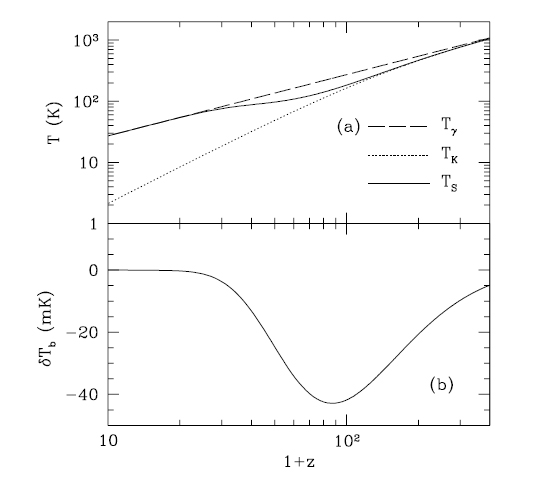
\includegraphics[width=0.95\linewidth]{Introduction/figures/dark_ages_global_spectrum.jpg}
\caption{(a) Plot of $T_S$, $T_\gamma$, and $T_K$ during the dark ages and (b) $\delta T_b$ during the same period given only collisional coupling from furlanetto et. al. \cite{furlanetto_2006}}
\label{Fig:da_global}
\end{center}
\end{figure}

\subsubsection{Dark Ages}
During the dark ages, the universe expanded at a rate defined by the Hubble parameter. Initially, the IGM was dense enough for Compton scattering between CMB photons and free electrons in the IGM to set \tk$=$\tg. But as the gas adiabatically expanded, thermal decoupling caused \tk to decrease. At this time, collisions between baryons in the IGM kept $x_K$ large, so that the spin temperature decreased below the CMB temperature. 

However, this coupling gradually decreased as the rate of collisions between baryons decreased, and the spin temperature increased back to match the CMB temperature. The process of cooling and decoupling created a dip in \ts, which most models predict should be centered around $z \sim 80 $ \cite{furlanetto_2006}. Figure \ref{Fig:da_global} shows one model prediction for the relevant temperatures including \tg, \tk, \ts and \dtb before star formation. 

At the same time, the first generation of stars began to form in the overdense regions of space. 

\subsubsection{Cosmic Dawn}
As the universe evolved during the dark ages, at the same time hierarchical structure formation led to the formation of more and more massive dark matter minihaloes. The first (PopIII.1) stars are believed to have formed in dark matter minihaloes with mass $\sim 10^6 - 10^8 M_{\odot}$, which $\Lambda$CDM simulations predict occurred around redshifts of $z \approx 20-30$ \cite{bromm_2013}. Formation of these first stars is considered the beginning of the $''$Cosmic Dawn$''$. 

%\textcolor{red}{Add figure of HII bubbles from aravind's review paper's reference.}

These first stars produce many UV photons, which ionize neutral hydrogen and create bubbles of ionized hydrogen (HII) around the stars. In addition, the stars also produce \lya  radiation, leading to coupling due to the Wouthuysen-Field effect. The total amount of coupling from the first stars $x_\alpha$ was shown in Equations \ref{Eq:xa} and \ref{Eq:pa} to be related to the \lya  photon intensity $J_\alpha$. This photon intensity is matched to emissivity of \lya  photons by the stars  plus the emissivity of photons in other Lyman transitions, which cascade down to affect the \lya  transition rate. 

The emissivity is heavily dependent on the rate of first star formation and the initial mass function (IMF) of PopIII stars. Some models suggest that PopIII stars may have a heavier IMF than that of younger stars, which would produce more \lya  photons per star \cite{natarajan_2014}. 

Meanwhile, x-ray photons were produced by two types of sources among the first Pop.III stars. One source was electrons accelerated by supernovae to relativistic speeds. When these electrons undergo inverse Compton scattering, x-ray photons are produced. The other source was high-mass x-ray binary stars, which occur when massive stars on the main sequence lose material through accretion onto a compact neighbor such as a neutron star, black hole or white dwarf star. 

These high energy photons heated the IGM through a combination of photoionization of Hydrogen or Helium and collisions with IGM components \cite{furlanetto_2006}. 

\begin{figure}[htb]
\begin{center}
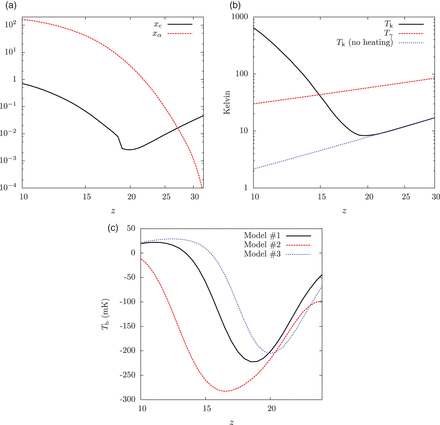
\includegraphics[width=0.95\linewidth]{Introduction/figures/ts_evolution.png}
\caption{Plots of (a) $x_K$ and $x_{\alpha}$, (b) $T_\gamma$ and $T_K$ with or without x-ray heating, and (c) $\delta T_b$ during the Cosmic Dawn for different models of star formation from natarajan et. al. \cite{natarajan_2014}}
\label{Fig:cd_global}
\end{center}
\end{figure}

Depending on the rate of x-ray heating compared to the rate of \lya coupling, the spin temperature is predicted to dip during the period where $x_k>0$ and \tk is less than \tg. By varying the model of first star formation that sets these two rates for PopIII stars, the exact shape of the dip in the spin temperature can be adjusted. Most models predict a dip centered around $z\sim20$, with a width of $0 \leq z \leq 10$ and a depth of $0\leq \Delta T \leq 300 mK$. 

Figure \ref{Fig:cd_global} shows a few models of global \dtb during the Cosmic Dawn, as well as some of the parameters that feed into the brightness temperature variance. These models were run by Aravind Natarajan using SIMFAST code \cite{simfast}\cite{21cmfast}\cite{natarajan_2014}.  

\begin{figure}[htb]
\begin{center}
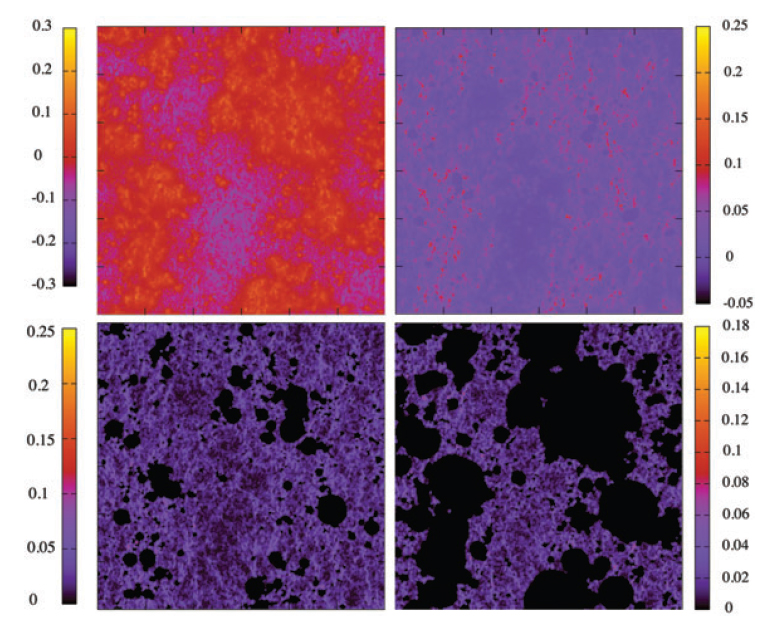
\includegraphics[width=0.95\linewidth]{Introduction/figures/reionization.jpg}
\caption{Snapshots at $z=$14,12,10,8 (from top left to bottom right) from a simulation run using SIMFAST from natarajan et. al. \cite{natarajan_2014}. The simulation shows the expected \dtb signal in units of Kelvin during the Epoch of Reionization. }
\label{Fig:eor}
\end{center}
\end{figure}

\subsubsection{Epoch of Reionization (EoR)}
As the kinetic temperature of the gas continued to rise, it reached the threshold where Equation \ref{Eq:dT_b} breaks down because the kinetic and spin temperatures of the gas are large enough that the approximation used for \tu is no longer applicable. At this point \dtb reaches a maximum because of saturation of the signal. 

Meanwhile, the propogation of x-ray photons through the IGM also began to ionize the hydrogen atoms starting in regions near the galaxies and spreading gradually throughout the IGM (see Figure \ref{Fig:eor}). This period of time is also known as the Epoch of Reionization (EoR) because the IGM is resuming the ionized state that it had in the early universe before the dark ages. 

Since the brightness temperature of the \cm signal is also proportional to the amount of neutral hydrogen ($x_{HI}$) present in the IGM, as shown in Equation \ref{Eq:dT_b}, the ionization process caused a gradual decrease in the average \cm signal. 

However, the gradual nature of the ionization means that there are interesting structures in the spatial distribution of the \cm signal during the EoR. The exact spatial distribution over time provides insight into the distribution of the PopIII stars, since larger stars produce more ionizing photons compared to the number of \lya  photons \cite{furlanetto_2006}. 

\subsubsection{Era of Acceleration}
In the modern universe post reionization, neutral Hydrogen gas in the IGM is limited to the regions around galaxies. This gas can still be mapped using the \cm signal, but the magnitude of the signal is much smaller than in previous eras. 

In this regime, mapping of the spectral structure can be done through intensity mapping. Intensity mapping is a process by which the signal from the neutral hydrogen can be measured in aggreggate around many galaxies. This is done with data that is collected in large voxels. Each voxel contains many galaxies and the \cm signal that is measured is the sum of the \cm signal from all the galaxies in that voxel \cite{masui_2012}.

\section{Measuring the \cm Signal}
After passing through the IGM at a given time, the \cm photons travel toward the earth. As they travel, the photons' frequencies are redshifted ($\nu_{meas} = \nu_{10}/(1+z)$) from their original frequencies. This shift allows us to measure a spectrum $\delta T_b (\nu)$, where $\nu$ is the frequency at which the signal is measured, corresponding to the redshift where the signal was produced. 

Measurements of the \cm spectrum are classified in two types. The first type aremeasurements of the sky-averaged spectrum \avgdtb, while the second type are measurements of the spatial fluctuations in the \cm spectrum ($\delta_{T_b} =  \delta T_b (\nu)/ T_b (\nu)$) using the power spectrum of the fluctuations ($ \tilde{ \delta_{T_b} } ( \vec{k} )$) \cite{natarajan_2014}. 

\begin{figure}[htb]
\begin{center}
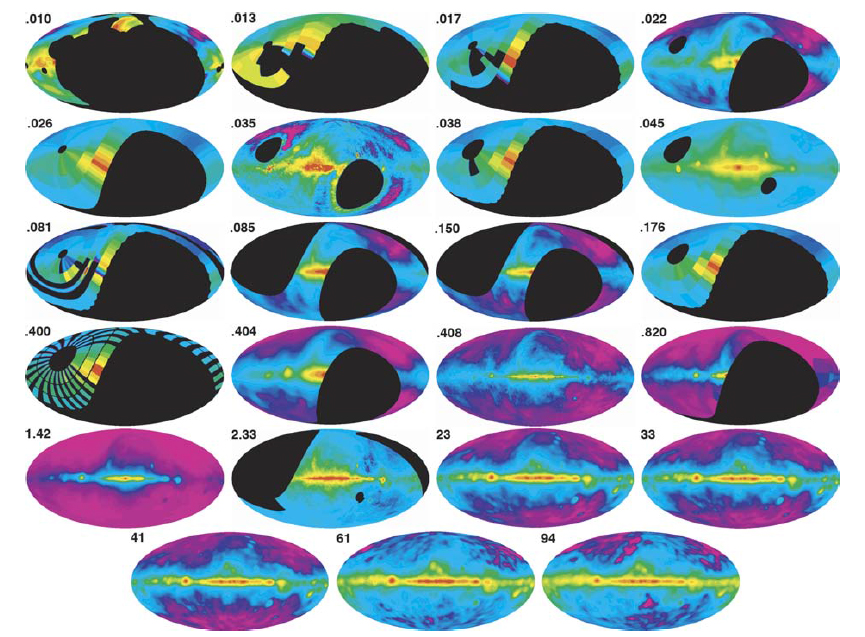
\includegraphics[width=0.95\linewidth]{Introduction/figures/GSM_maps.jpg}
\caption{Plots of radio sky measurements used to construct the Global Sky Model \cite{GSM_model} of radio foregrounds. The number in the upper left corner of each plot is the frequency (in GHz) at which the map data was collected, while the color scale is the log of the sky temperature in Kelvin.}
\label{Fig:GSM_maps}
\end{center}
\end{figure}

\subsection{Non-Cosmological Foregrounds}
One of the greatest challenges of making any \cm measurements is the presence of foregrounds in the data. These foregrounds include any signals on the sky that aren't related to the CMB brightness temperature (\tb) and its variance due to the IGM. Foreground signals come from astrophysical sources which emit in the low frequency radio band ($\nu \leq \nu_{10}$), interference from Earth's ionosphere, and radio frequency interference (RFI) from man-made sources. I will discuss RFI in Chapter \ref{Ch:RFI} and ionospheric impacts in Chapter \ref{Ch:Iono}, so in this section I will focus on astrophysical foregrounds. 

For $\nu \leq \nu_{10}$ the dominant astrophysical foreground is synchrotron radiation from the Milky Way Galaxy. This radiation comes from free electrons in the galaxy and has a strongly sloping spectrum \cite{furlanetto_2006}, as shown in Equation \ref{Eq:T_sky}. 

\begin{equation}\label{Eq:T_sky}
T_{sky} \approx 180 \Big( \frac{\nu}{180 MHz} \Big)^{-2.6} K
\end{equation}

Maps of the astrophysical foregrounds have been made at a number of frequencies, including the $''$Haslam$''$ map at 408 MHz and the WMAP maps (after removal of the CMB signal) at 23,33,41,61 and 94 GHz. These maps are shown in Figure \ref{Fig:GSM_maps}. A model of the foregrounds from $10 MHz-100 GHz$ was constructed using the maps, as outlined in de Oliveira-Costa et al \cite{GSM_model}. This sky model is commonly used for foreground assessment and even calibration by \cm experiments. A discussion of how the model is used in the SCI-HI project can be found in Section \ref{Sec:model}. 

\subsection{Average (Global) Frequency Spectrum (\avgdtb)}
In order to make a measurement of \avgdtb, experiments need to be designed that measure the total sky brightness temperature spectrum ($T_{Sky}$) over a wide range of frequencies. These experiments will measure the combination of signals collected by an antenna:

\begin{equation}
T_{ant} = T_{fg} + T_b +T_{sys}+T_{RFI} = T_{Sky} + T_{sys}
\end{equation}

where $T_{fg}$ is the astrophysical foreground signal, $T_{RFI}$ is the man-made signal, $T_{sys}$ is the system temperature, and \tb is the brightness temperature from the CMB. The system temperature $T_{sys}$ will be a combination of thermal noise and instrument noise. Thermal noise is set by the radiometer equation ($T_{thermal} = T_{ant}/\sqrt{BW \tau}$), where $BW$ is the system bandwidth and $\tau$ is the integration time \cite{carroll2007}. Instrument noise comes from the electronics in the system (such as the amplifiers). 

Extracting the \cm brightness temperature spectrum requires removing all of the other terms in the data. Different strategies have been proposed for removing these signals, but all of them rely on the fact that the other signals have a different type of spectral structure than the \cm signal. I will discuss one such strategy for foreground removal with the SCI-HI experiment in Section \ref{Sec:fore}. 

\subsection{Fluctuation Power Spectrum ($ \tilde{ \delta_{T_b} } ( \vec{k} )$)}
Like the \avgdtb experiments, power spectrum measurements will also be dominated by foregrounds. Unlike the \avgdtb experiments, these foregrounds are dominated by specific galactic and extragalactic point sources. However, like the Milky Way galaxy, these sources have a smooth spectrum that can be fitted with a power law; although each point source follows a different power law. 

There are a number of different specific foreground removal strategies that have been developed, including principal component analysis \cite{masui_2012}\cite{switzer_2013}. All of these strategies rely on the removal of the dominant foregrounds thanks to their smooth spectra. The \cm signal is left behind when the foregrounds are removed because it will have significant structure in frequency, as each frequency corresponds to  the signal from a different set of galaxies in the intensity map. 

\section{Hydrogen \cm Cosmology Experiments}
There are a number of experiments specifically designed to measure the \cm global signal or power spectrum. These experiments are either currently gathering data or are still under development. Preliminary constraints on the \cm signals have been placed for different cosmological eras, and future measurements should continue to tighten those constraints such that we will have a good detection of the \cm global signal and power spectrum during the Dark Ages, Cosmic Dawn, Epoch of Reionization and Era of Acceleration. 

\subsection{Global Experiments}
The experiments that are trying to measure the \avgdtb signal are focused on redshifts where \dtb is large and/or has a large first derivative, which is expected to occur during the Dark Ages, Cosmic Dawn, and the Epoch of Reionization. EDGES \cite{bowman_2008} is a single antenna experiment focused on frequencies $100-200 MHz$. It has placed limits on the duration of reionization using the width of the \cm global signal emission bump during the Epoch of Reionization. 

LEDA \cite{leda}\cite{bernardi_2014} and DARE \cite{burns_2011} are currently under development, and are targeting the Dark Ages and Cosmic Dawn. LEDA is designed to operate on the ground using a combination of an interferometer and a single antenna, while DARE intends to launch a satellite in orbit around the moon with a single antenna. 

Both of these experiments have large budgets of over 1 million dollars and require significant resources and technology development. In contrast, the EDGES experiment is on a much smaller scale and can be deployed in the field with minimal infrastructure. 

\subsubsection{SCI-HI Experiment}
We were inspired by the EDGES experiment to develop a similar system focusing on a different part of the \cm spectrum ($40 \leq \nu \leq 130 MHz$) and going after the Cosmic Dawn signal. This experiment is the SCI-HI experiment, and will be the main focus of the rest of this thesis.  

\subsection{Mapping Experiments}
Experiments which seek to measure the \cm power spectrum are typically many-element interferometers, each with a different antenna design and configuration. Early projects, including the GMRT-EoR \cite{paciga_2013} project, made use of existing telescopes to make measurements. Meanwhile, a number of projects were designed and constructed such as the Precision Array for Probing the Epoch of Reionization (PAPER) \cite{pober_2013}\cite{jacobs_2014}, the Murchison Widefield Array (MWA) \cite{bernardi_2013}\cite{tingay_2012}, and the Low Frequency Array for Radio Astronomy (LOFAR) \cite{jelic_2014}\cite{lofar}. These projects have put first constraints on the power spectrum during the Epoch of Reionization. 

Future projects targeting the Epoch of Reionization signal include the Hydrogen Epoch of Reionization (HERA) \cite{hera}\cite{bernardi_2014} array and the Square Kilometer Array (SKA) \cite{ska}.

Beyond the EoR projects, there are a number of power spectrum projects focusing on lower redshifts during the Era of Acceleration. The \cm signal targeted by these projects is much smaller than the EoR signal, but the foregrounds at these frequencies are also much smaller. First constraints on the power spectrum were placed by the GBT-IM project \cite{masui_2012}\cite{switzer_2013}, which used the Green Bank Telescope to make a map of a few degree patch of sky and construct a power spectrum from that map. 

Like with the EoR experiments, full sky mapping requires a dedicated project. One such project is the Canadian Hydrogen Intensity Mapping Experiment (CHIME) \cite{shaw_2014}\cite{chime}, currently under development. CHIME uses a unique cylindrical interferometer design to map the sky. 

Chapter \ref{Ch:Planet} includes some discussion of the Green Bank Telescope and CHIME, and how they were used in a public outreach project for educating the public on \cm cosmology. 



\chapter{Teaching \cm Cosmology to the Public}\label{Ch:Planet}

\section{Overview}
\section{Storyboard and Script}

\subsection{Introduction}
\subsection{\cm Science}
\subsection{Radio Telescopes}
\subsection{Green Bank Telescope and Intensity Mapping}
\subsection{CHIME Telescope}
\subsection{Science Goals}

\section{On-site Filming}

\subsection{Green Bank, WV}
\subsection{Penticton, BC, Canada}

\section{Working in the Planetarium Environment}

\subsection{Technology}
\subsection{Visual Differences}

\section{Audio Production}

\subsection{Narration}
\subsection{Music and Sound Effects}

\section{Feedback and Evaluation}



\chapter{SCI-HI System Development}\label{Ch:System}

\section{Overview}
$''$Sonda Cosmologica de las Islas para la Deteccion de Hidrogeno Neutro$''$ (SCI-HI) is an experiment which seeks to measure the \cm global spectrum during the end of the Dark Ages and the Cosmic Dawn before reionization. As such, SCI-HI instrument was designed to meet several distinct contraints:

\begin{enumerate}
\item The design must be low cost (under \$ 10,000 \textcolor{red}{Is this the right range?}).

\item The design must be low power (under \textcolor{red}{What value should this be?}) and be able to run with an independent power source separate from external supplies. 

\item The design must be simple and easy to deploy to remote locations. 

\item The design must be broad-band to cover the wide bandwidth of interest ($30-140$ MHz).

\end{enumerate}

\begin{figure}[htb]
\begin{center}
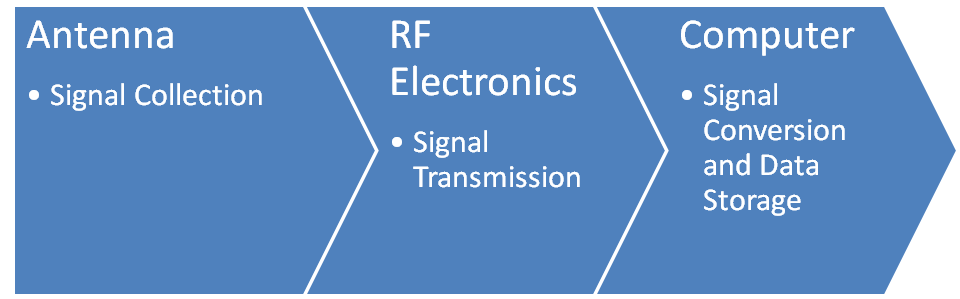
\includegraphics[width=0.9\linewidth]{SCIHI_system/figures/basic_block_diagram.png}
\caption{Basic Block Diagram of the SCI-HI instrument.}
\label{Fig:basic_block_diagram}
\end{center}
\end{figure}

In order to meet these constraints, the instrument design was broken down into three categories based upon their purpose in the overall design (see Figure \ref{Fig:basic_block_diagram}). These categories are an antenna for signal collection, radio frequency (RF) electronics for signal transmission, and a computer for signal processing and storage.

\section{Antenna}
When designing an instrument for radio astronomy, one of the big challenges is finding an antenna design that fits the particular needs of a given experiment. 

\subsection{Design Considerations}
For the SCI-HI experiment, the key properties for the antenna selection were the bandwidth and stability of the antenna beam pattern and impedance (S-parameters) over frequency. 

\textcolor{red}{Here I will add a brief discussion of antenna design including some of the key parameters for an antenna in general and why they are significant. }

\begin{figure}[htb]
\centering
\begin{minipage}[b]{0.45\textwidth}
\centering
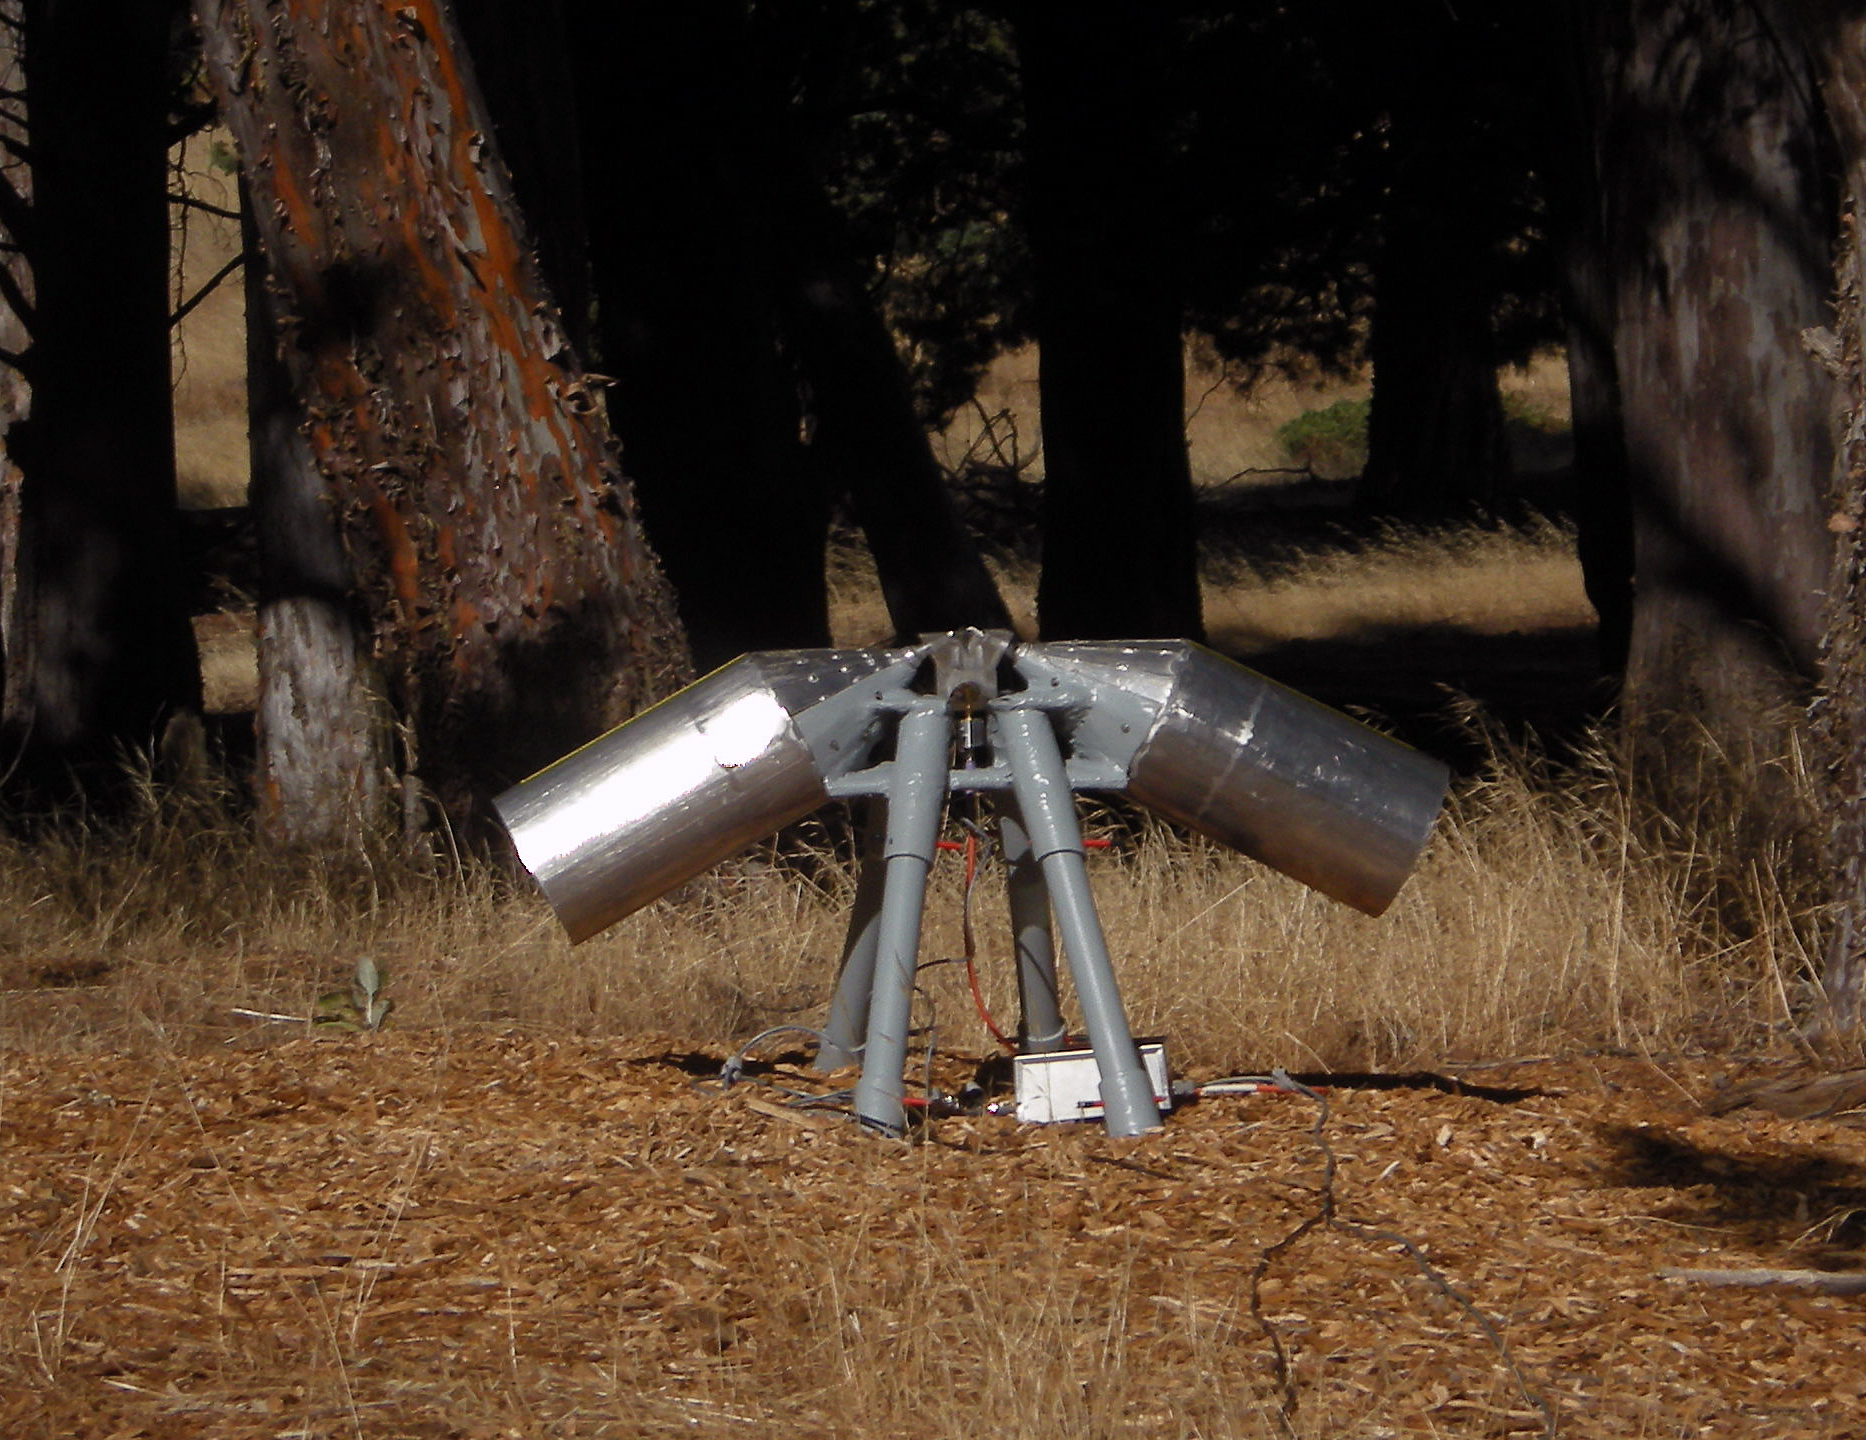
\includegraphics[width=0.95\linewidth]{SCIHI_system/figures/trombone_guad_small.jpg}
\caption{Trombone Antenna setup in its smallest (highest center frequency) configuration.}
\label{Fig:trombone_small}
\end{minipage}%
\begin{minipage}[b]{0.02\textwidth}
\hspace{1cm}
\end{minipage}%
\begin{minipage}[b]{0.51\textwidth}
\centering
\includegraphics[width=0.95\linewidth]{SCIHI_system/figures/trombone_pgh_zoom.jpg}
\caption{Trombone Antenna setup in its largest (lowest center frequency) configuration.}
\label{Fig:trombone_large}
\end{minipage}
\end{figure}

\subsection{First Stage Antenna}
Initially, we started with a simple $''$Trombone$''$ antenna. This design is a dipole with fat, angled elements over a ground plane (see Figures \ref{Fig:trombone_small} and \ref{Fig:trombone_large}). Changing the frequency range of the antenna simply required shifting the length of the dipole elements and their position above the ground plane. 

\begin{figure}[htb]
\centering
\begin{minipage}[b]{0.53\textwidth}
\centering
\includegraphics[width=0.95\linewidth]{SCIHI_system/figures/trombone_mount.jpg}
\caption{Mounting for the Trombone antenna, with lucite mount point and fiberglass support structure. }
\label{Fig:trombone_mount}
\end{minipage}%
\begin{minipage}[b]{0.02\textwidth}
\hspace{1cm}
\end{minipage}%
\begin{minipage}[b]{0.41\textwidth}
\centering
\includegraphics[width=0.95\linewidth]{SCIHI_system/figures/trombone_guad_adj.jpg}
\caption{Changing the Trombone antenna configuration from small to large.}
\label{Fig:trombone_adj}
\end{minipage}
\end{figure}

\subsubsection{Antenna Construction}
The trombone shapes were constructed out of welded aluminum with a lucite mounting block at the connection point of the two cones (see Figure \ref{Fig:trombone_mount}), The dipoles and mounting block were supported with a structure constructed out of fiberglass and PVC tubes. The entire system was placed above a ground plane composed of metal mesh (aka chicken wire) over a small ($\sim9 m^2$) area and long wire extensions ($\sim10 m$) extending out from the center like a spider web. 

Tuning the trombone length was accomplished with an external tube that slid over the main dipole elements (see Figure \ref{Fig:trombone_adj}), while adjusting the height of the trombone was done using the support legs (PVC pipes with variable heights).

The Trombone antenna was used throughout the initial stages of the SCI-HI project, including deployments at Green Bank in West Virginia (Figure \ref{Fig:trombone_gbt}), the Zona del Silencio in Mexico (Figure \ref{Fig:trombone_zds}), Algonquin Radio Observatory in Canada (Figure \ref{Fig:trombone_alg}), and Isla Guadalupe in Mexico (Figure \ref{Fig:trombone_guad}). For more discussion of these sites, see Chapter \ref{Ch:RFI}.

\begin{figure}[htb]
\centering
\begin{minipage}[b]{0.48\textwidth}
\centering
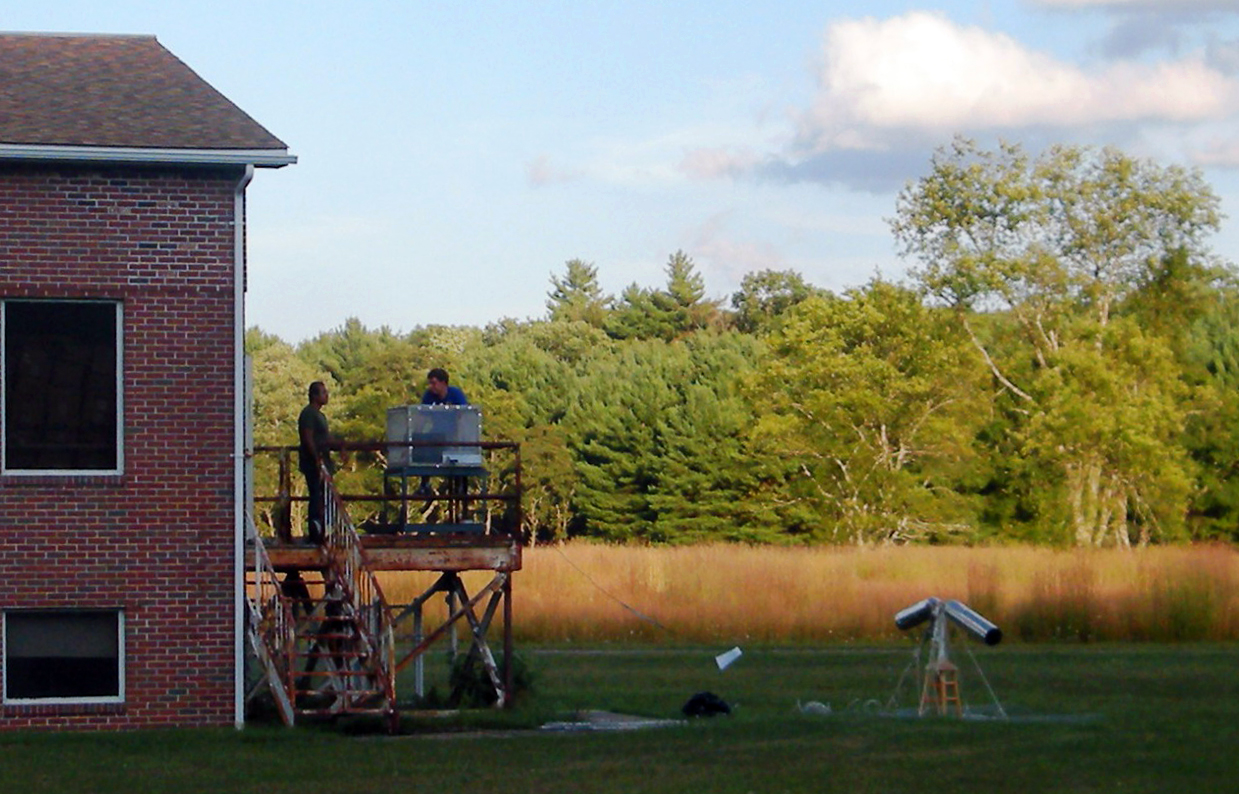
\includegraphics[width=0.95\linewidth]{SCIHI_system/figures/trombone_gbt.jpg}
\caption{SCI-HI setup with trombone antenna on site at Green Bank in August 2011.}
\label{Fig:trombone_gbt}
\end{minipage}%
\begin{minipage}[b]{0.02\textwidth}
\hspace{1cm}
\end{minipage}%
\begin{minipage}[b]{0.46\textwidth}
\centering
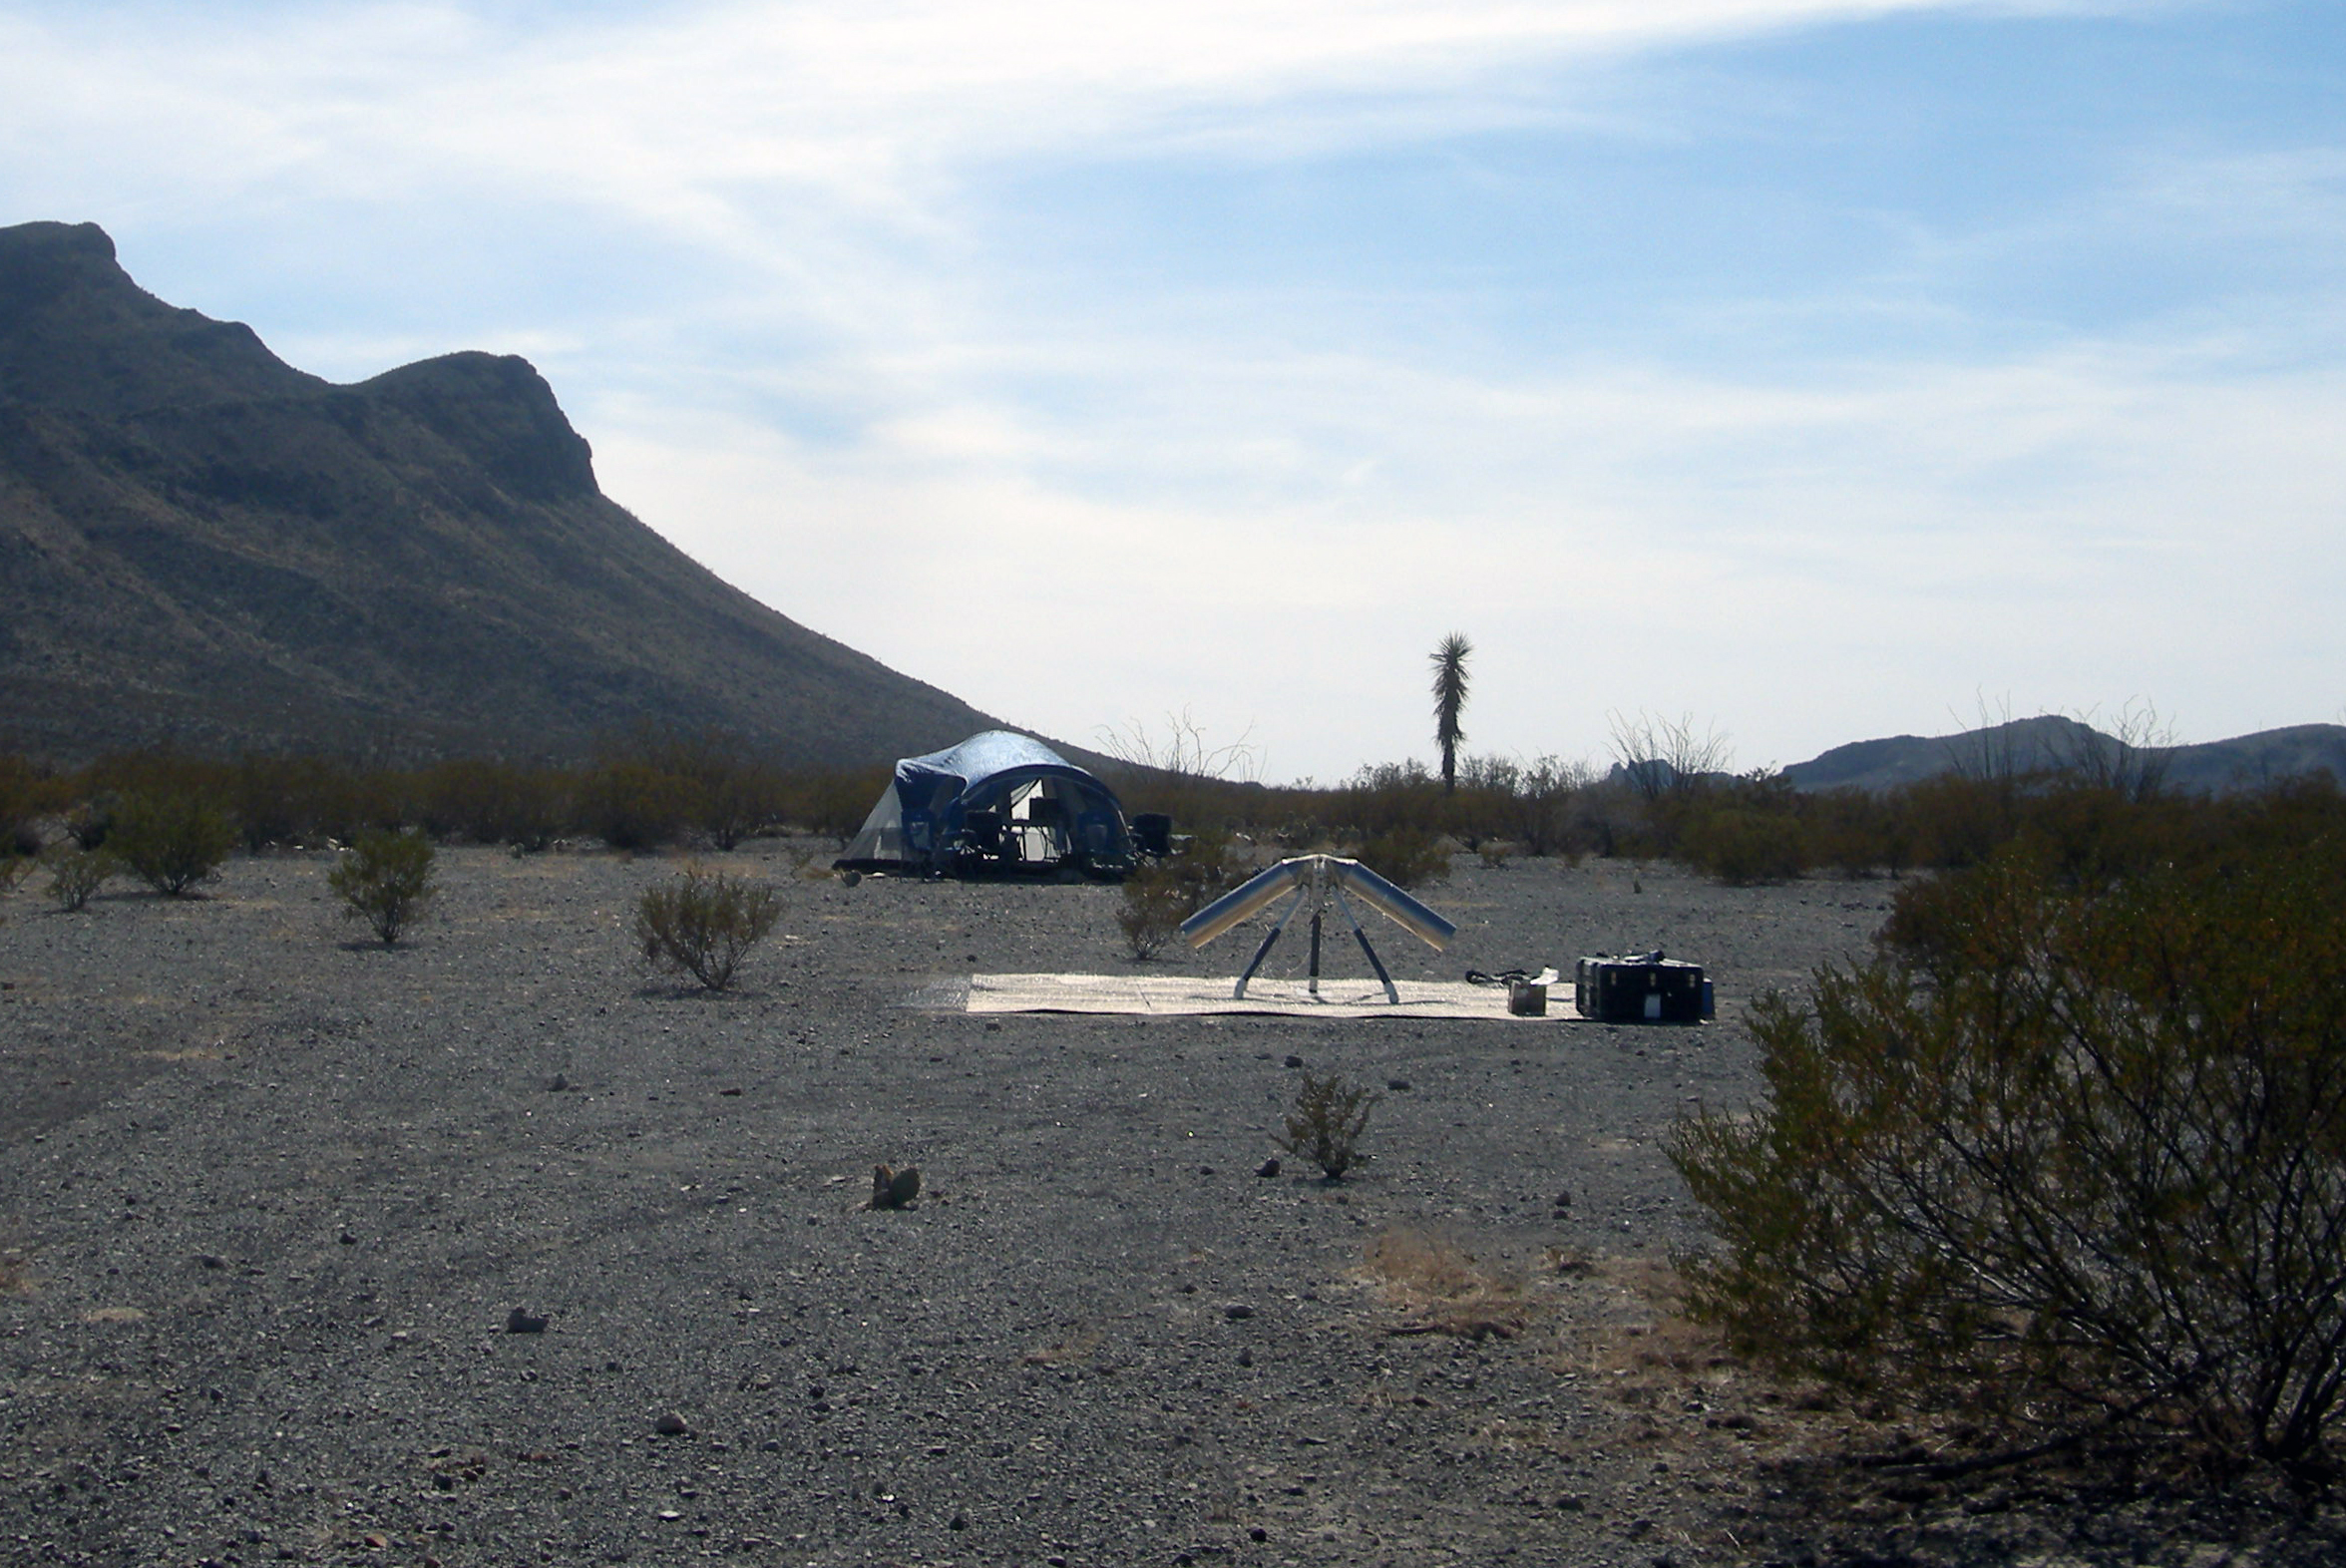
\includegraphics[width=0.95\linewidth]{SCIHI_system/figures/trombone_sys_ZdS.jpg}
\caption{SCI-HI setup with trombone antenna on site at the Zona del Silencio in January 2012.}
\label{Fig:trombone_zds}
\end{minipage}
\end{figure}

\begin{figure}[htb]
\centering
\begin{minipage}[b]{0.52\textwidth}
\centering
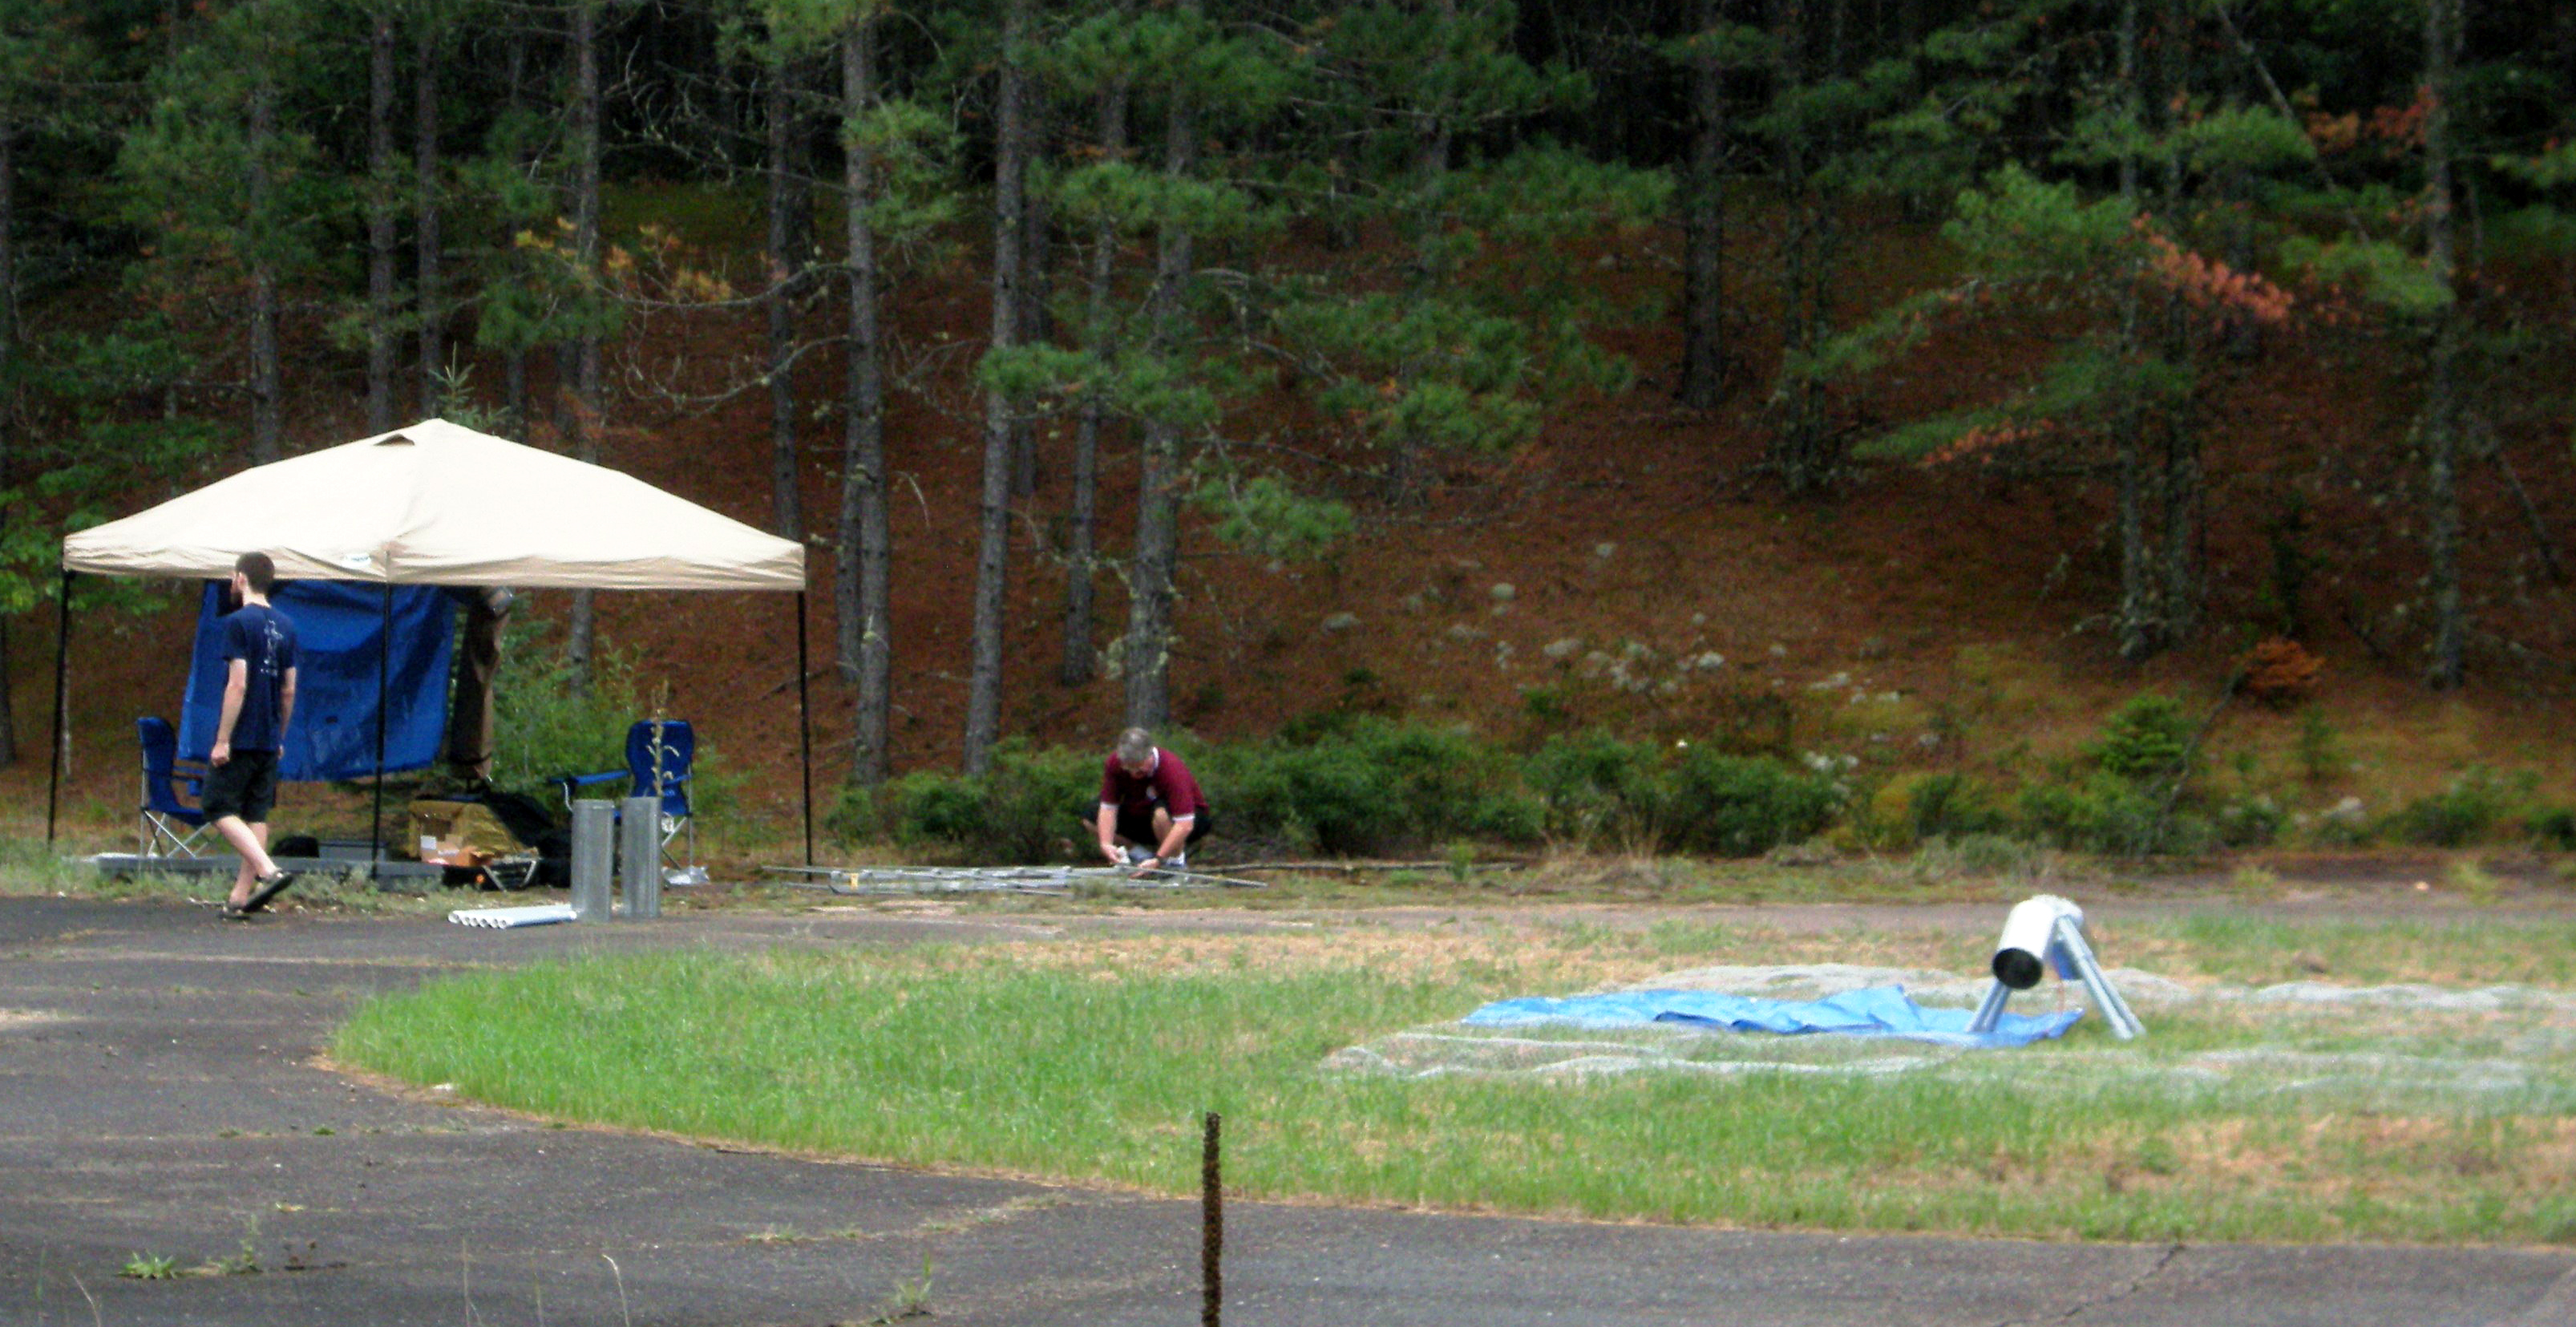
\includegraphics[width=0.95\linewidth]{SCIHI_system/figures/trombone_alg_sys.jpg}
\caption{SCI-HI setup with trombone antenna on site at the Algonquin Radio Observatory in August 2012.}
\label{Fig:trombone_alg}
\end{minipage}%
\begin{minipage}[b]{0.02\textwidth}
\hspace{1cm}
\end{minipage}%
\begin{minipage}[b]{0.42\textwidth}
\centering
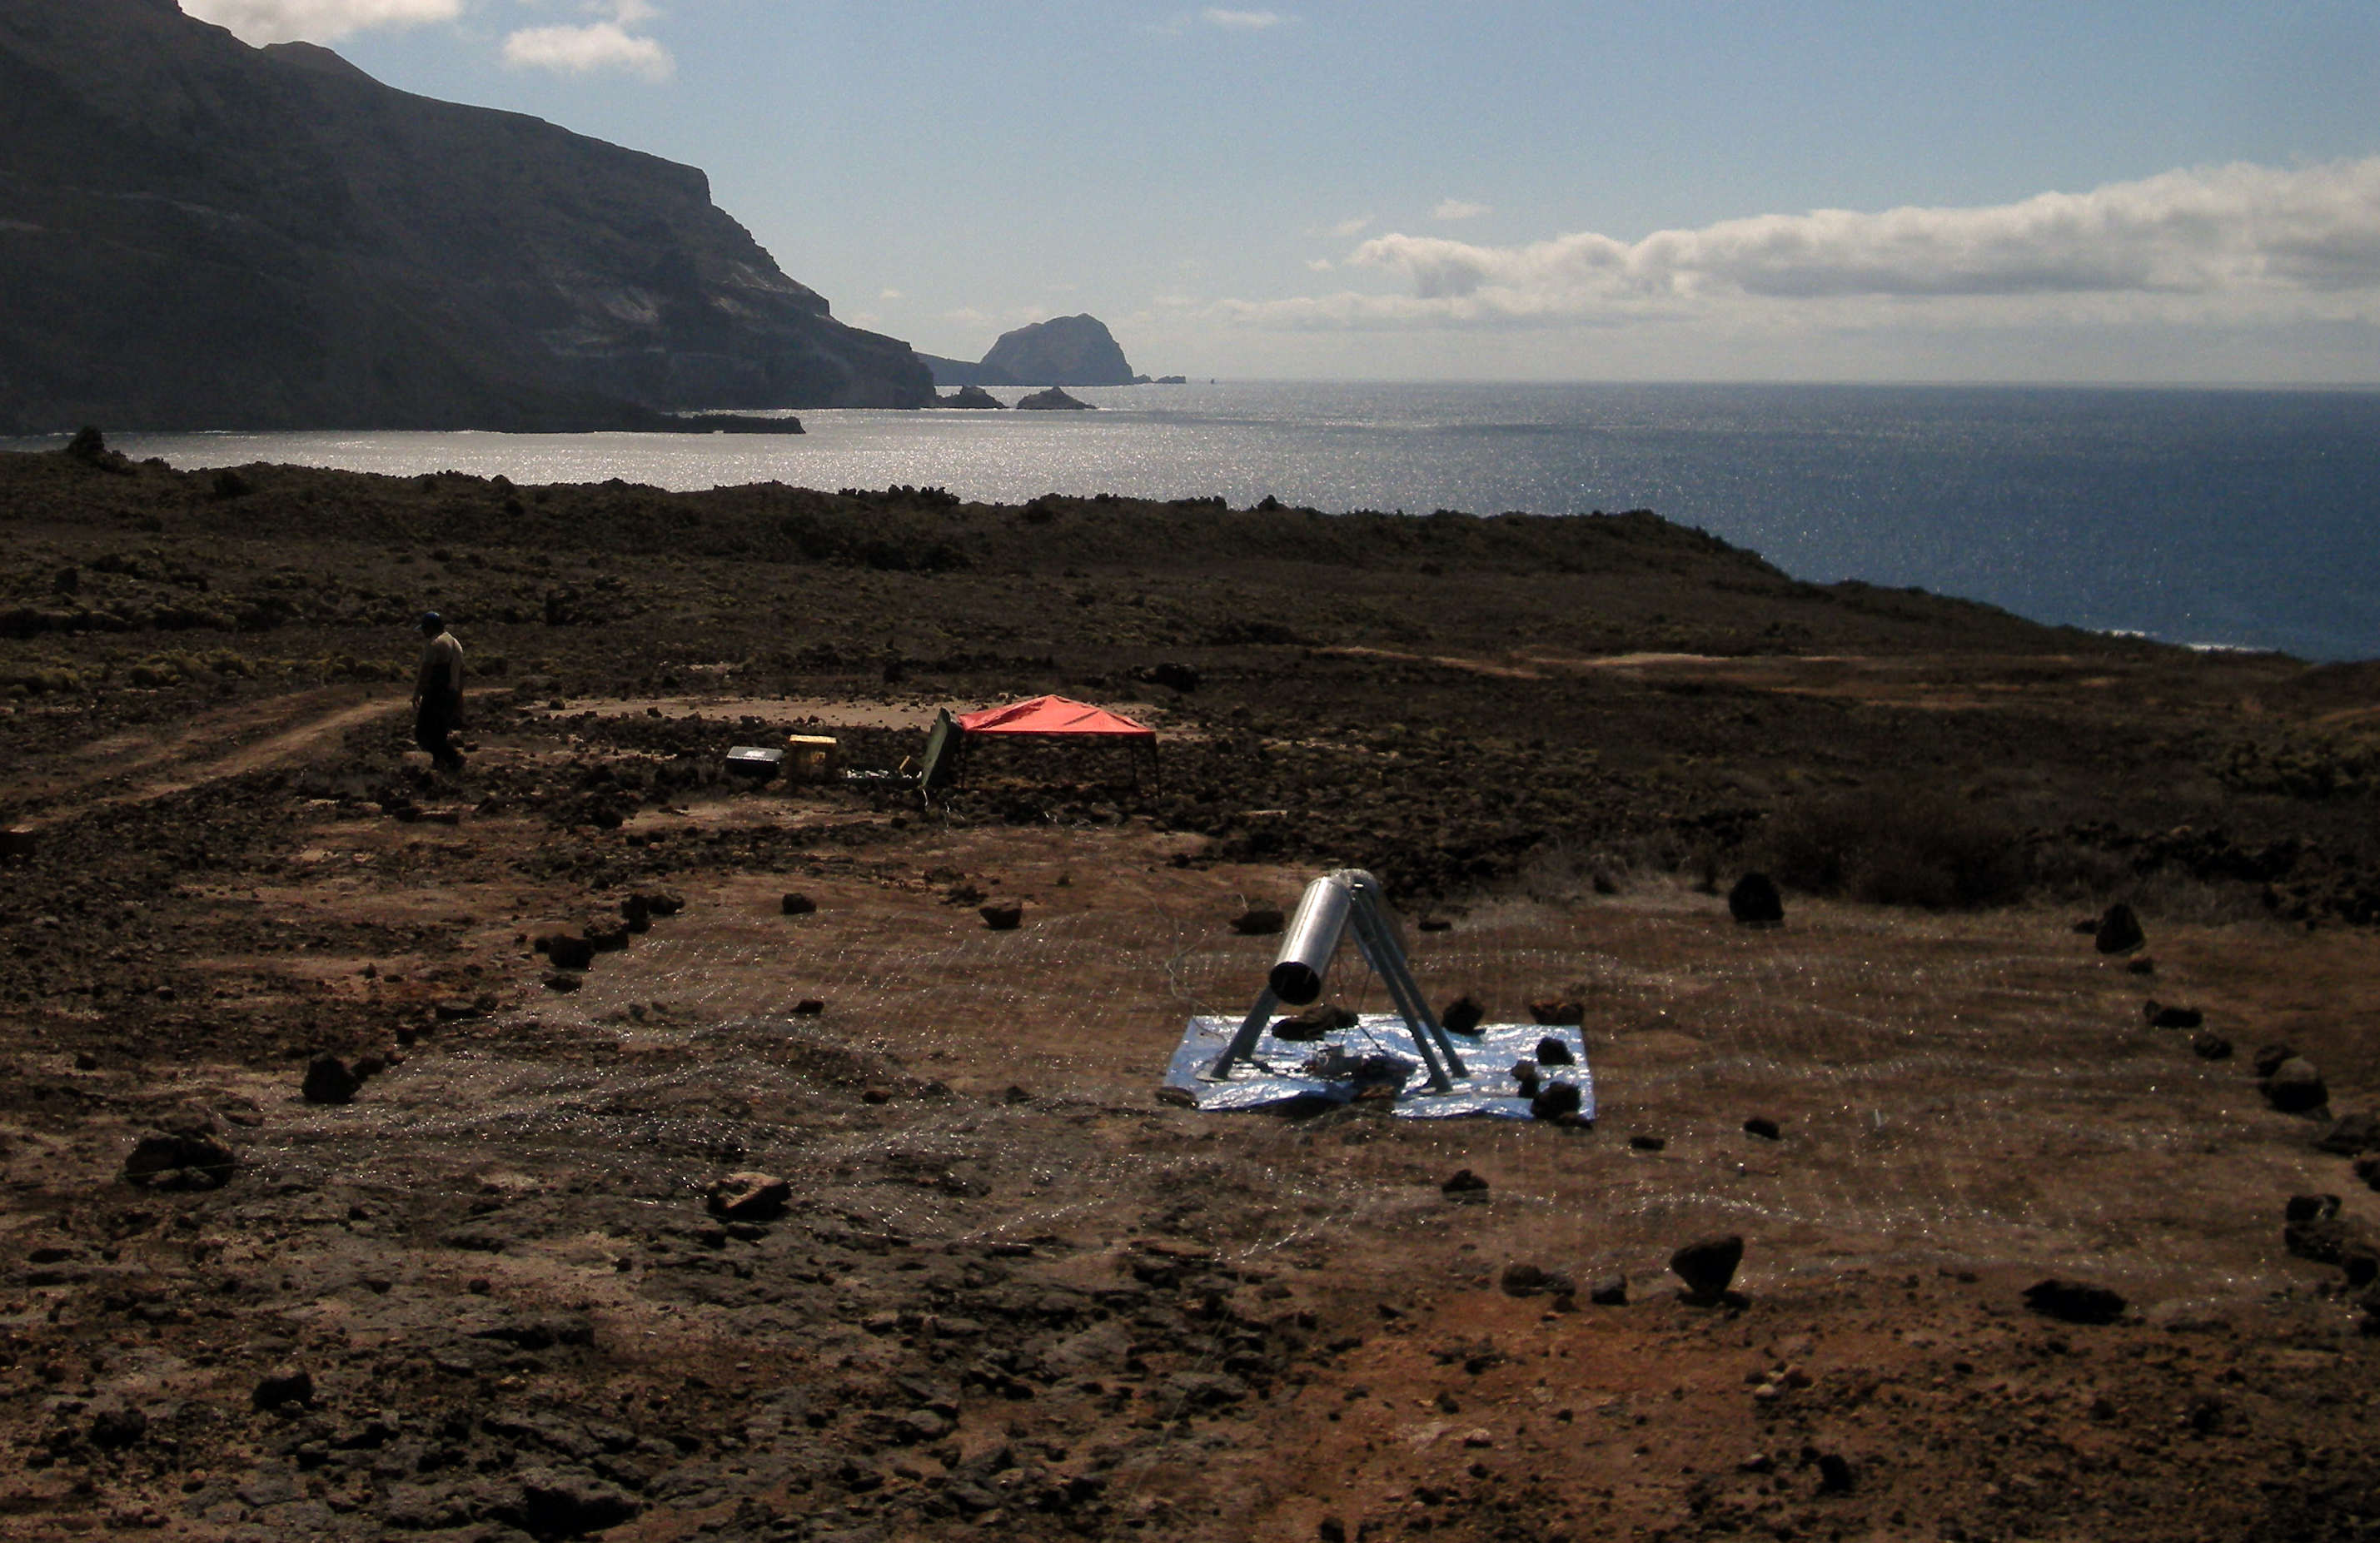
\includegraphics[width=0.95\linewidth]{SCIHI_system/figures/trombone_sys_guad.jpg}
\caption{SCI-HI setup with trombone antenna on site at Isla Guadalupe in October 2012.}
\label{Fig:trombone_guad}
\end{minipage}
\end{figure}

\subsubsection{Antenna Simulation}
Simulating the Trombone antenna indicated some problems with the design, including significant structure in the antenna beam and S-parameters. \textcolor{red}{Add image/details of Amy's simulation results.}

\subsection{HIbiscus Antenna Design}

Because of the problems we had with the trombone design, we decided to shift our antenna design in a new direction based upon our expectations from the literature (\textcolor{red}{Need to add specific references for different antenna types}). We tested several antenna designs in simulation, including the four-square design used in the EDGES experiment \cite{rogers_2012}. This testing was done using FEKO, a finite element computational electromagnetics software package.\footnote{https://www.feko.info/}

Based on the FEKO simulation results we settled on a design that used the EDGES design as a starting point, but changed the exact shapes of the four squares. We took each square and turned it into an incliclined petal composed of three trapezoidal shapes. Each shape was connected to its neighbors on the petal, but had a different angle with respect to the ground. Additional panels were added to each side of the petal to create a strip line with a fixed gap between the petals. The entire antenna was then placed a distance above a flat ground plane. We call this design a HIbiscus antenna. 

\textcolor{red}{Add either pictures or simulation images for antenna shape details.}

We found that the shape parameters that were most significant in affecting antenna performance were the strip line gap width and the height of the antenna with respect to the ground plane. 


\begin{figure}[htb]
\centering
\begin{minipage}[b]{0.50\textwidth}
\centering
\includegraphics[width=0.95\linewidth]{SCIHI_system/figures/model_test_tabitha.jpg}
\caption{Testing a model HIbiscus antenna in the Project REAL Chamber. }
\label{Fig:hibiscus_scale_tabitha}
\end{minipage}%
\begin{minipage}[b]{0.02\textwidth}
\hspace{1cm}
\end{minipage}%
\begin{minipage}[b]{0.44\textwidth}
\centering
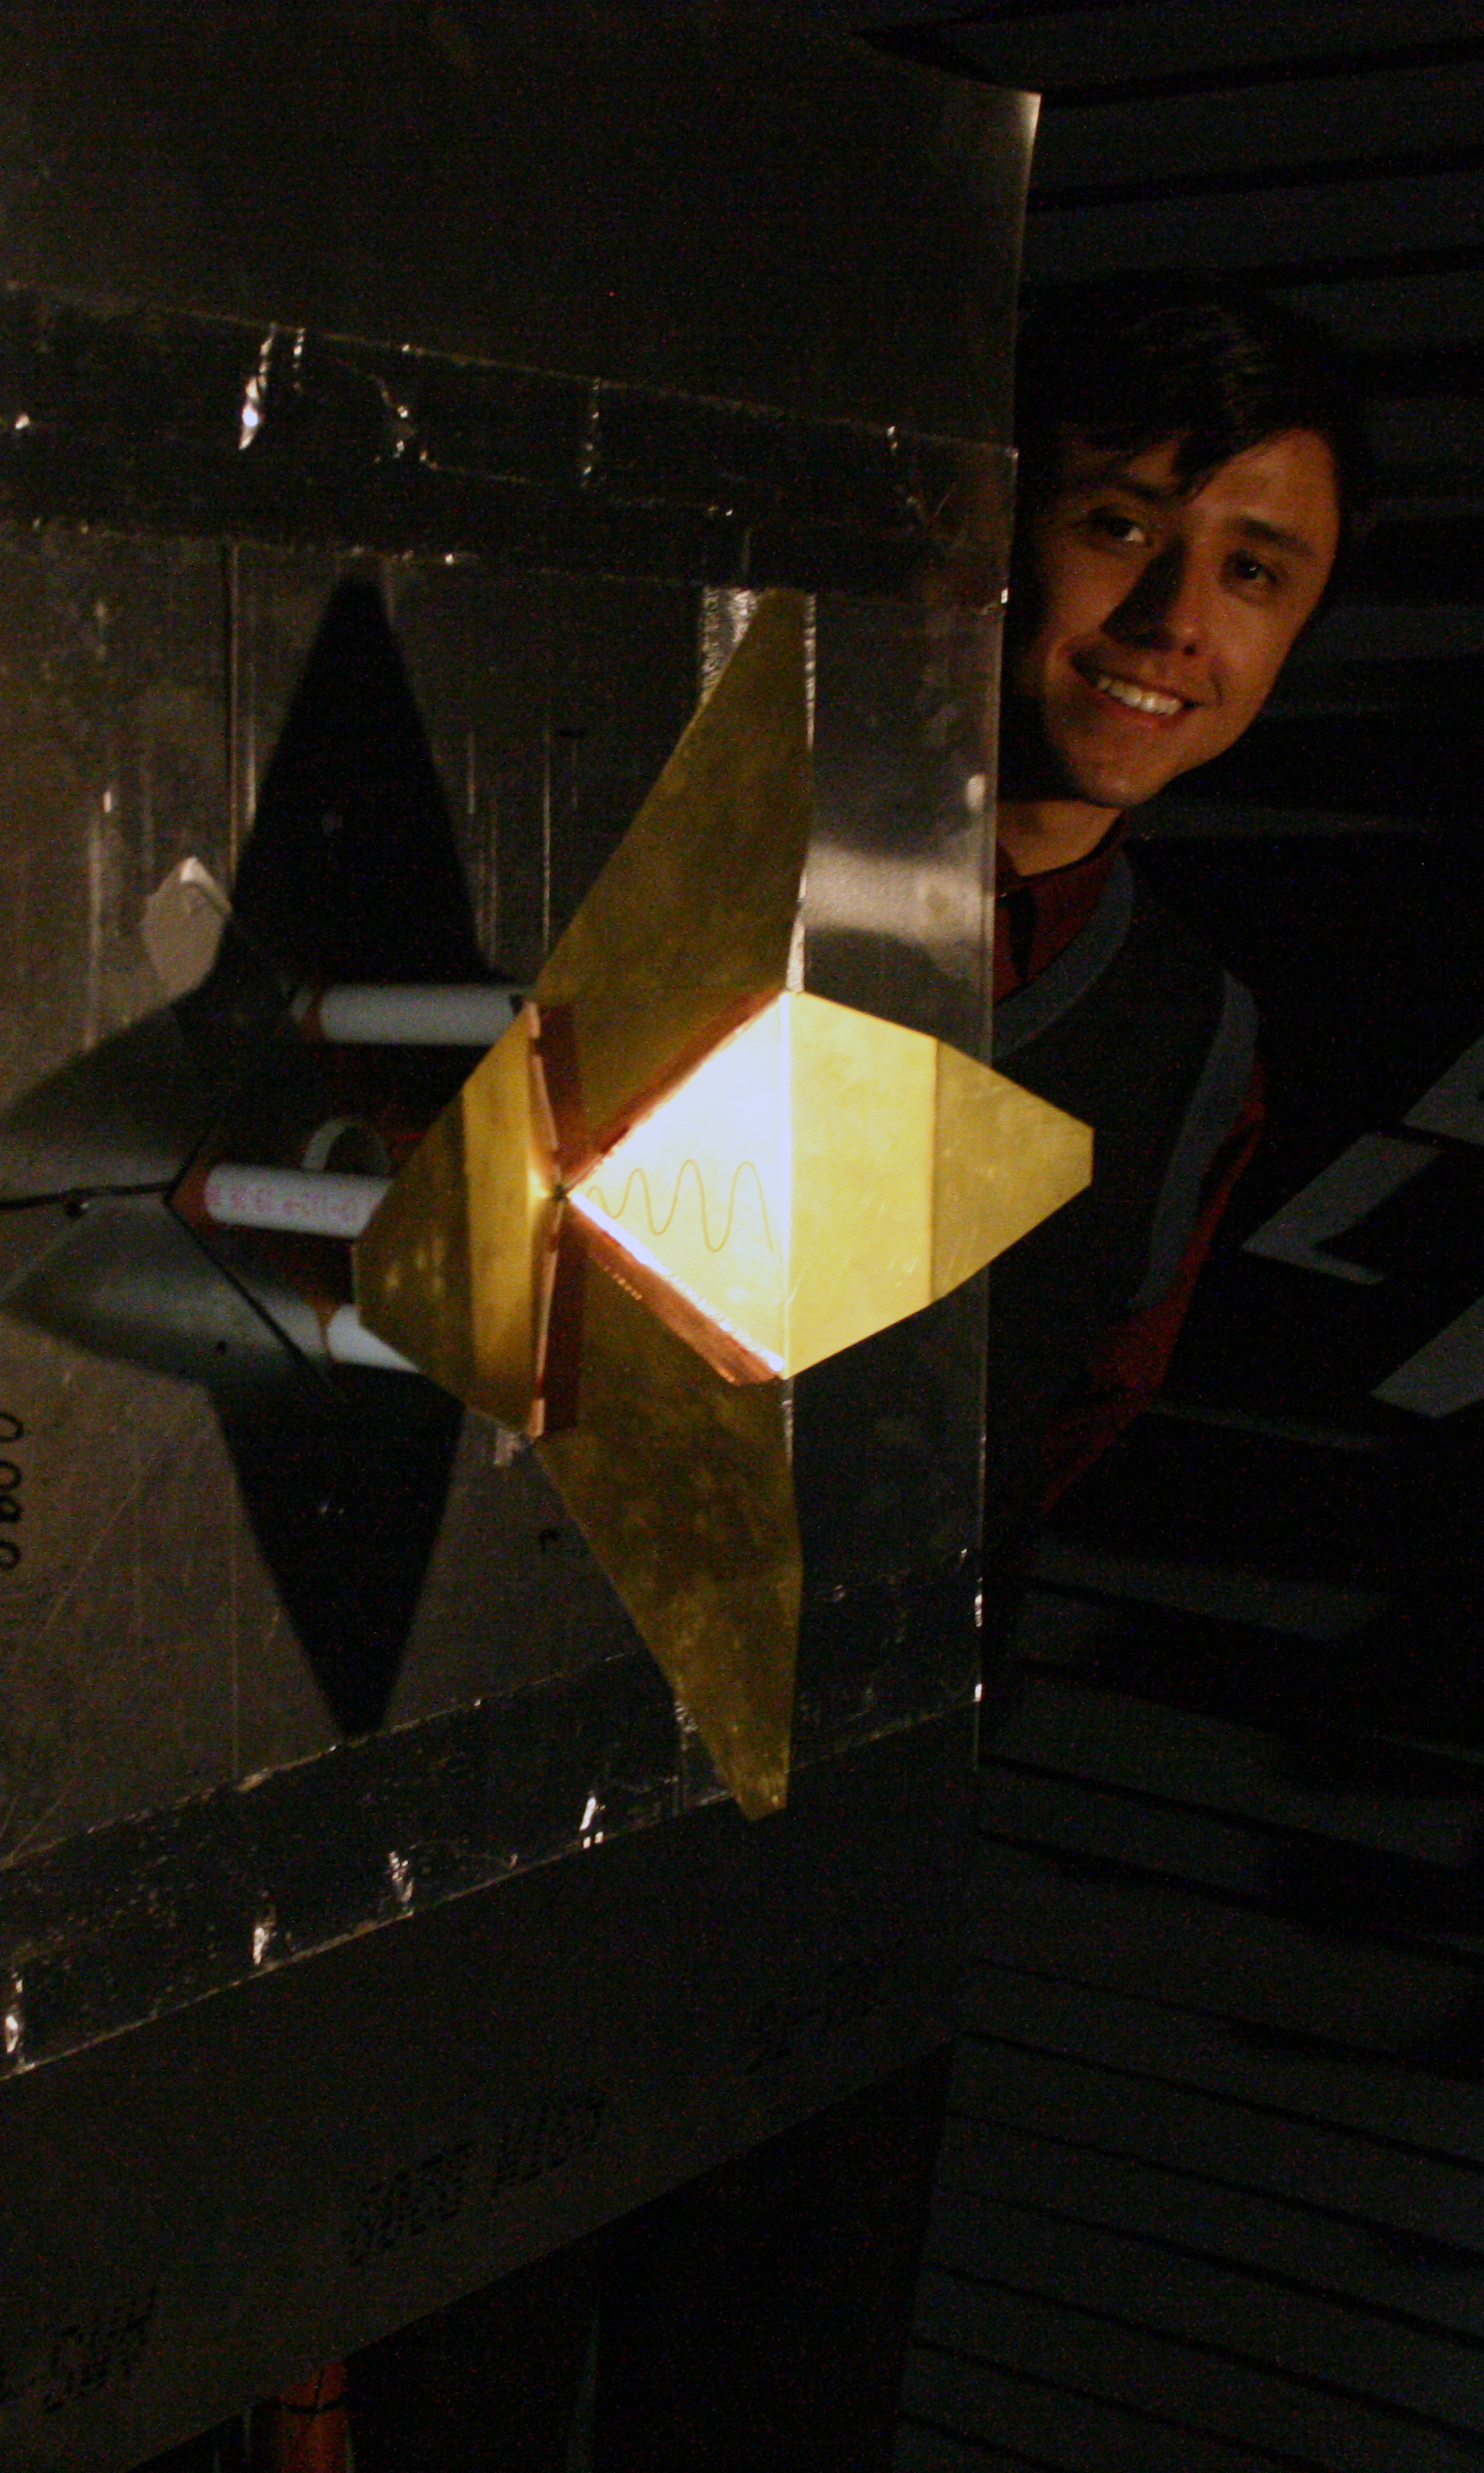
\includegraphics[width=0.95\linewidth]{SCIHI_system/figures/model_test_jose.jpg}
\caption{Scale model test with a different HIbiscus antenna model.}
\label{Fig:hibiscus_scale_jose}
\end{minipage}
\end{figure}

\subsubsection{Scale Model Testing}
In order to test our simulation to see if it matched the real antenna performance, we built a set of scaled HIbiscus designs tuned for higher frequencies around 400 MHz. This allowed us to use an antenna range to measure the antenna beam shape and s-parameters. 

We used the Project REAL\footnote{http://www.preal.ece.cmu.edu/} (Remote Educational Antenna Laboratory) facility at Carnegie Mellon University to measure the antenna response of different scaled HIbiscus models, as is shown in Figures \ref{Fig:hibiscus_scale_tabitha} and \ref{Fig:hibiscus_scale_jose}. By incrementally adjusting the strip line gap width and antenna height we were able to tune the antenna scale model to optimize these critical parameters in a real design. 

Using the scale model data, we were also able to edit the antenna simulation to better match the actual antenna response, providing us with an antenna simulation dataset that was closer to reality. 

\textcolor{red}{Here there will be some paragraphs about the exact simulation and scale model measurements including plots of impedence and antenna pattern.}

\begin{figure}[htb]
\centering
\begin{minipage}[b]{0.43\textwidth}
\centering
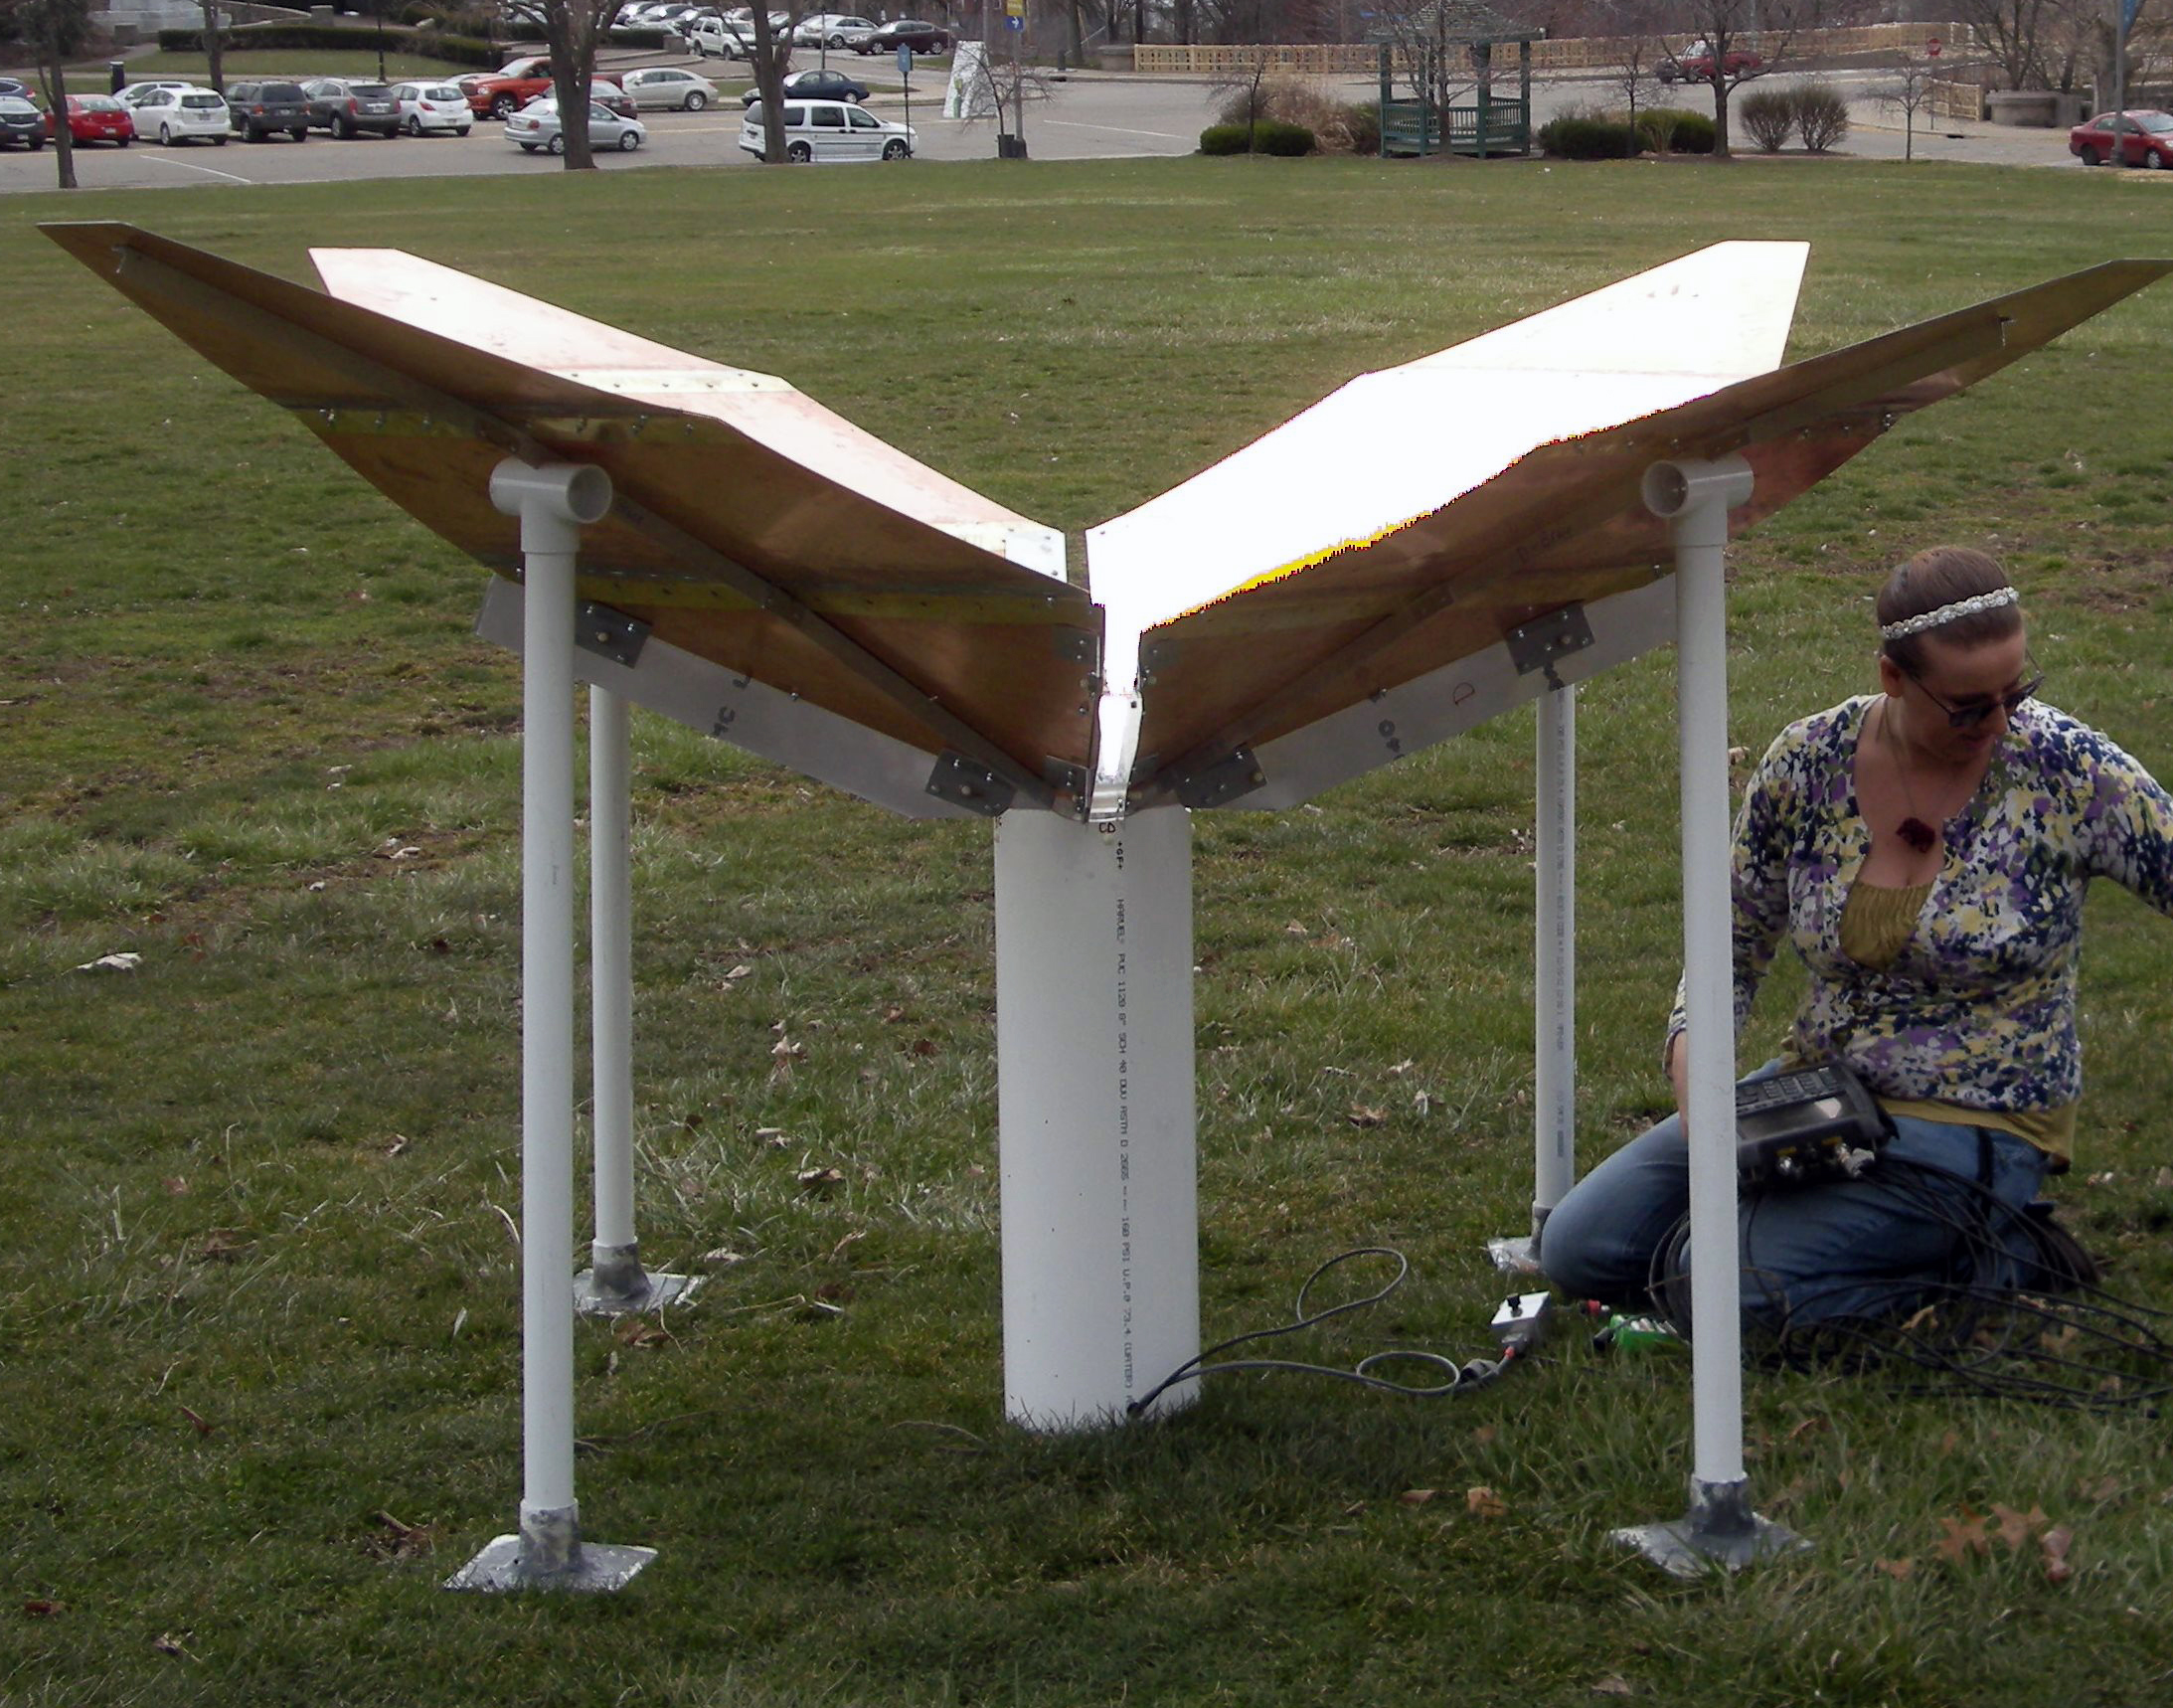
\includegraphics[width=0.95\linewidth]{SCIHI_system/figures/HIbiscus_pgh_imp.jpg}
\caption{HIbiscus antenna scaled for 70 MHz as it was setup during s-parameter testing at CMU. }
\label{Fig:hibiscus_first}
\end{minipage}%
\begin{minipage}[b]{0.02\textwidth}
\hspace{1cm}
\end{minipage}%
\begin{minipage}[b]{0.51\textwidth}
\centering
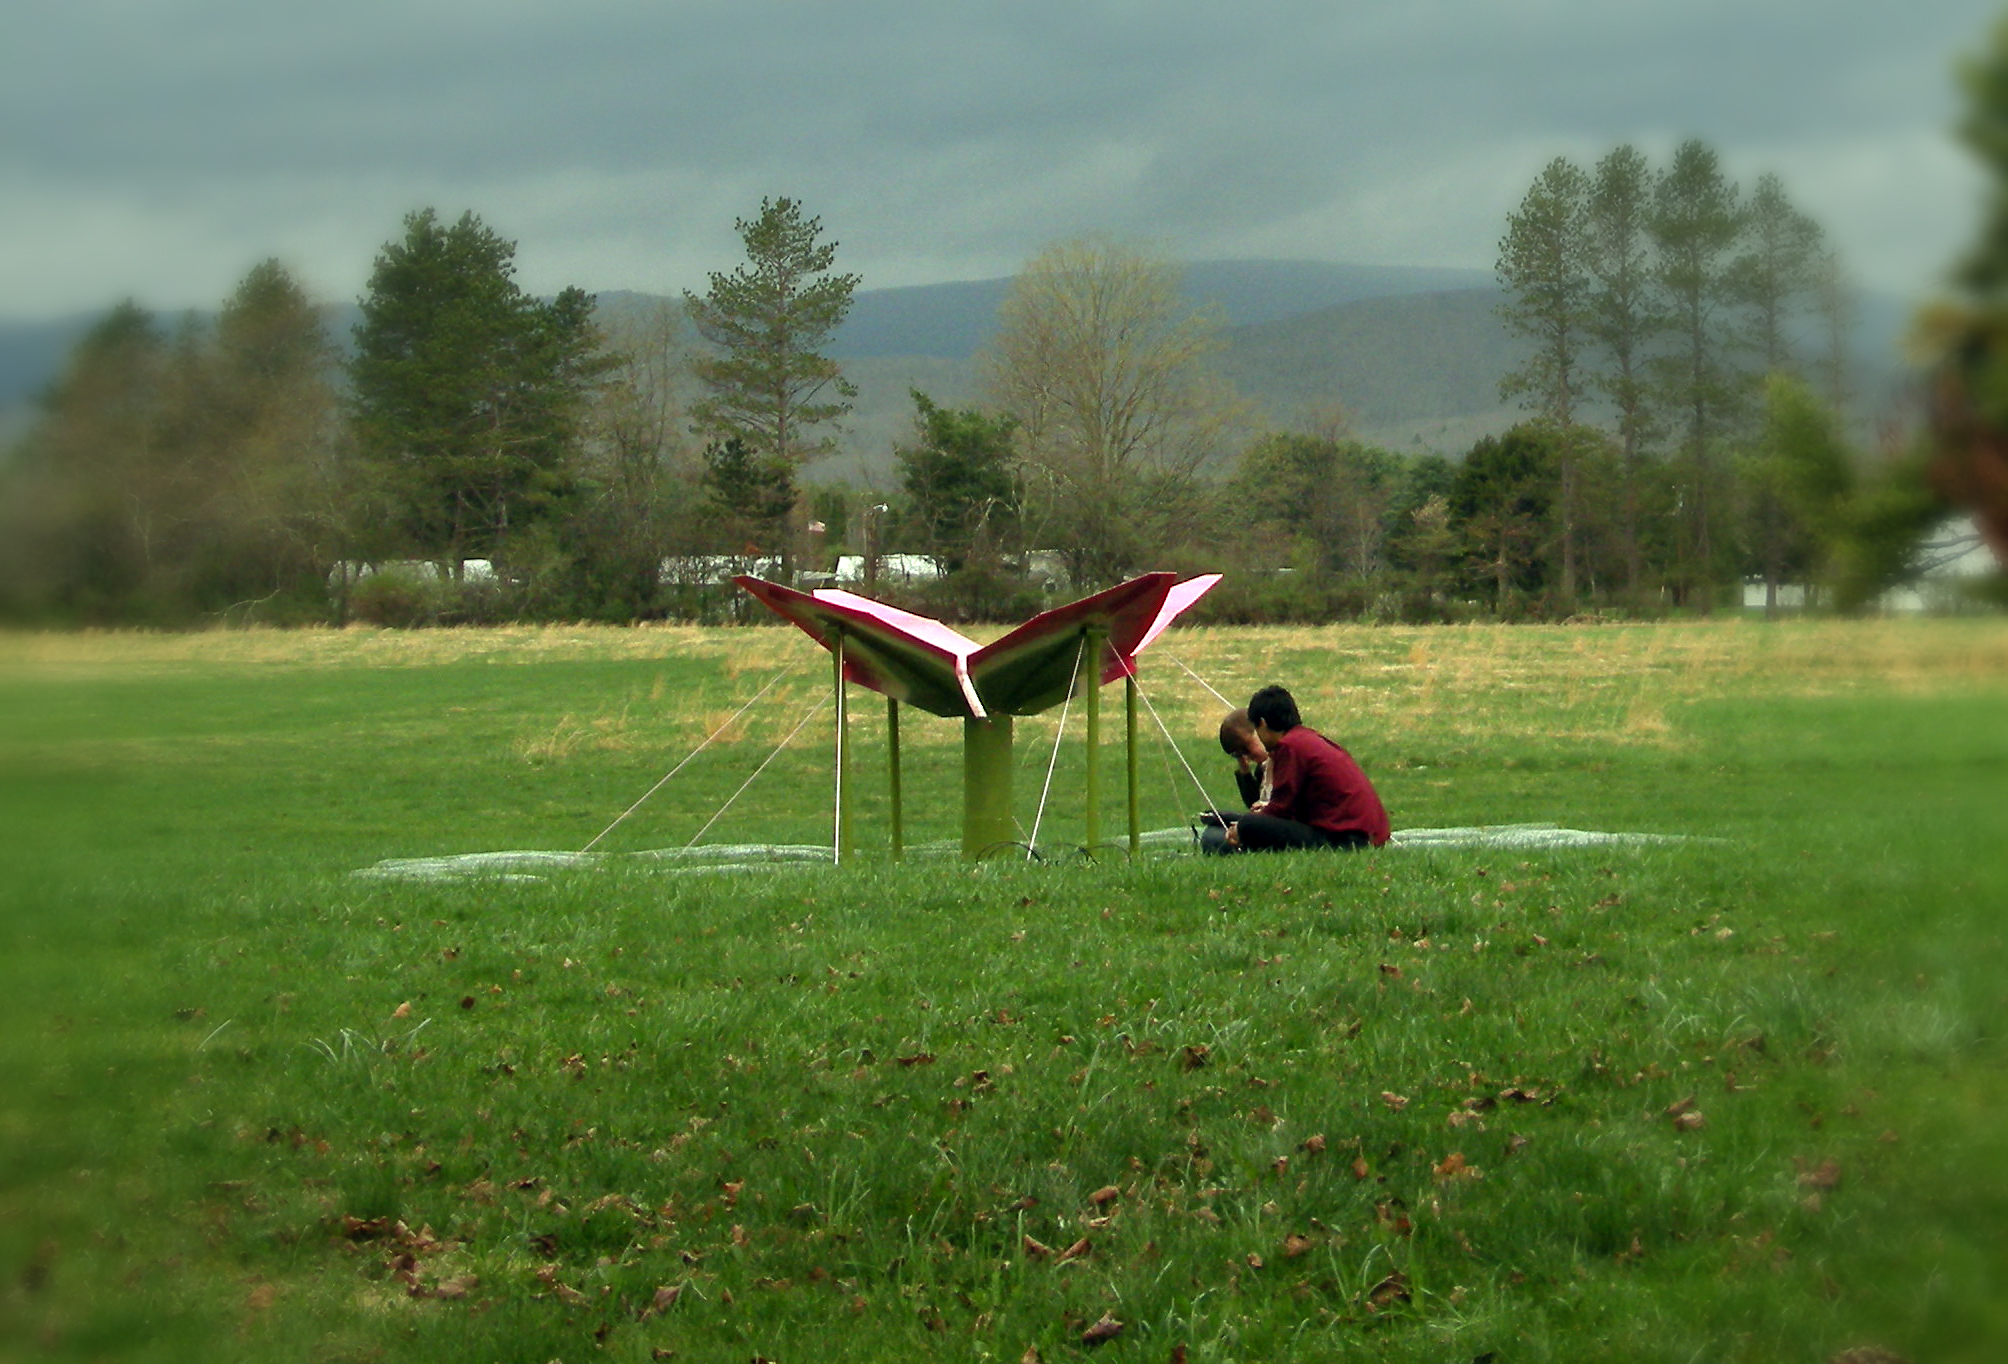
\includegraphics[width=0.95\linewidth]{SCIHI_system/figures/HIbiscus_gbt.jpg}
\caption{HIbiscus antenna scaled for 70 MHz setup for s-parameter testing on site at Green Bank.}
\label{Fig:hibiscus_gbt}
\end{minipage}
\end{figure}

\subsection{HIbiscus Antenna Construction}

\subsubsection{Initial Assembly}
Once we had a design finalized, we set out to construct a HIbiscus antenna with its center frequency tuned to 70 MHz (in the middle of the SCI-HI observation band).

To construct the antenna petals, we started with large sheets of printed circuit board (pcb) material (see Figure \ref{Fig:hibiscus_pcb}). This material is a sheet of fiberglass sandwiched by two thin sheets of copper. We cut each of the trapezoidal shapes out of the pcb material, then added brass flanges to connect the shapes. Underneath the center line of each petal we placed a rib made out of aluminum angle with the appropriate bends to match the angles between trapezoids. Finally, the strip line panels were added using aluminum sheets soldered to some of the trapezoids (see Figure \ref{Fig:hibiscus_solder}). The entire system is bolted together using screws, and can be separated into parts for travel. 

\begin{figure}[htb]
\centering
\begin{minipage}[b]{0.39\textwidth}
\centering
\includegraphics[width=0.95\linewidth]{SCIHI_system/figures/HIbiscus_pcb_cut.jpg}
\caption{HIbiscus antenna pcb panels being cut. }
\label{Fig:hibiscus_pcb}
\end{minipage}%
\begin{minipage}[b]{0.02\textwidth}
\hspace{1cm}
\end{minipage}%
\begin{minipage}[b]{0.55\textwidth}
\centering
\includegraphics[width=0.95\linewidth]{SCIHI_system/figures/HIbiscus_solder.jpg}
\caption{Soldering the strip line to the HIbiscus antenna panels.}
\label{Fig:hibiscus_solder}
\end{minipage}
\end{figure} 

In order to keep the petal separation even and correct, lucite spacers were placed between each of the petals (see Figure \ref{Fig:hibiscus_spacer}). In addition, a lucite mount was built for the connection points at the center of the antenna (see Figure \ref{Fig:hibiscus_center}). The entire system was raised above the ground using a set of five PVC pipe legs; a central column and one leg for each petal (see Figure \ref{Fig:hibiscus_first}). 

\begin{figure}[htb]
\centering
\begin{minipage}[b]{0.52\textwidth}
\centering
\includegraphics[width=0.95\linewidth]{SCIHI_system/figures/HIbiscus_strip_line.jpg}
\caption{Sight line down one of the strip lines for the HIbiscus antenna with spacers in place.}
\label{Fig:hibiscus_spacer}
\end{minipage}%
\begin{minipage}[b]{0.02\textwidth}
\hspace{1cm}
\end{minipage}%
\begin{minipage}[b]{0.42\textwidth}
\centering
\includegraphics[width=0.95\linewidth]{SCIHI_system/figures/HIbiscus_center_point.jpg}
\caption{Center of the HIbiscus antenna with spacers and center mount block in place.}
\label{Fig:hibiscus_center}
\end{minipage}
\end{figure}

Beyond the antenna structure, a ground plane was also required to keep the ground pattern constant in time. Like with the Trombone, we used a ground plane made out of chicken wire. In this case, our simulations showed us that a $\sim 100 m^2$ square ground plane was sufficient for our application. The entire system (antenna plus ground plane) was anchored to the ground to minimize the wind impact on the system. Each of the four support legs had an anchoring rope (see Figure \ref{Fig:hibiscus_gbt}), and the chicken wire was also anchored with many stakes. 

With the antenna constructed, we could test that it matched our scale model measurements in terms of its s-parameters. To do this, we set up the antenna outdoors and made measurements with a portable Vector Network Analyzer. Measurements had to be made outdoors because the wavelengths corresponding to the SCI-HI frequencies ($40-130$ MHz) are $\sim$1-10 meters. This large wavelength scale means that reflections from the boundaries of a room can change antenna s-parameters, so accuracy in measurement requires the outdoor setting. Figures \ref{Fig:hibiscus_first} and \ref{Fig:hibiscus_gbt} show examples of how we made this measurement at CMU and Green Bank.

\textcolor{red}{Here I'll add a paragraph with S11 data using VNA and explanation.}

\subsubsection{Travelling with the Antenna}
In order to use the HIbiscus antenna on-site at remote locations, it needed to be transportable to those locations and easily assembled upon arrival. The physical construction of the antenna was designed to match this requirement in a number of ways. 

First, the entire system was made as lightweight as possible. This was accomplished by using the pcb material, which was much lighter and stiffer than the equivalent sheet metal panels would be. 

Second, the system was designed in segments so it could be assembled and disassembled and packed into small bags. Each petal separated out into three trapezoids that were screwed together for assembly, but could be packed as mostly flat sheets. The lucite spacers and mount were attached to the petals using screws and could be removed and packed for travel, as were the PVC pipe supports. 

Third, the entire system was arranged for travel in three suitcases (plus an extra bag for the ground plane chicken wire). These suitcases were small and light enough to be checked as regular baggage on commercial airlines. 

\begin{figure}[htb]
\begin{center}
%\centering
%\begin{minipage}[b]{0.47\textwidth}
%\centering
\includegraphics[width=0.95\linewidth]{SCIHI_system/figures/HIbiscus_70mhz_lab.jpg}
\caption{New HIbiscus antenna scaled for 70 MHz as laid out in the lab. Scale model in picture for comparison.}
\label{Fig:hibiscus_70}
\end{center}
\end{figure}

%\end{minipage}%
%\begin{minipage}[b]{0.02\textwidth}
%\hspace{1cm}
%\end{minipage}%
%\begin{minipage}[b]{0.47\textwidth}
%\centering

\begin{figure}[htb]
\begin{center}
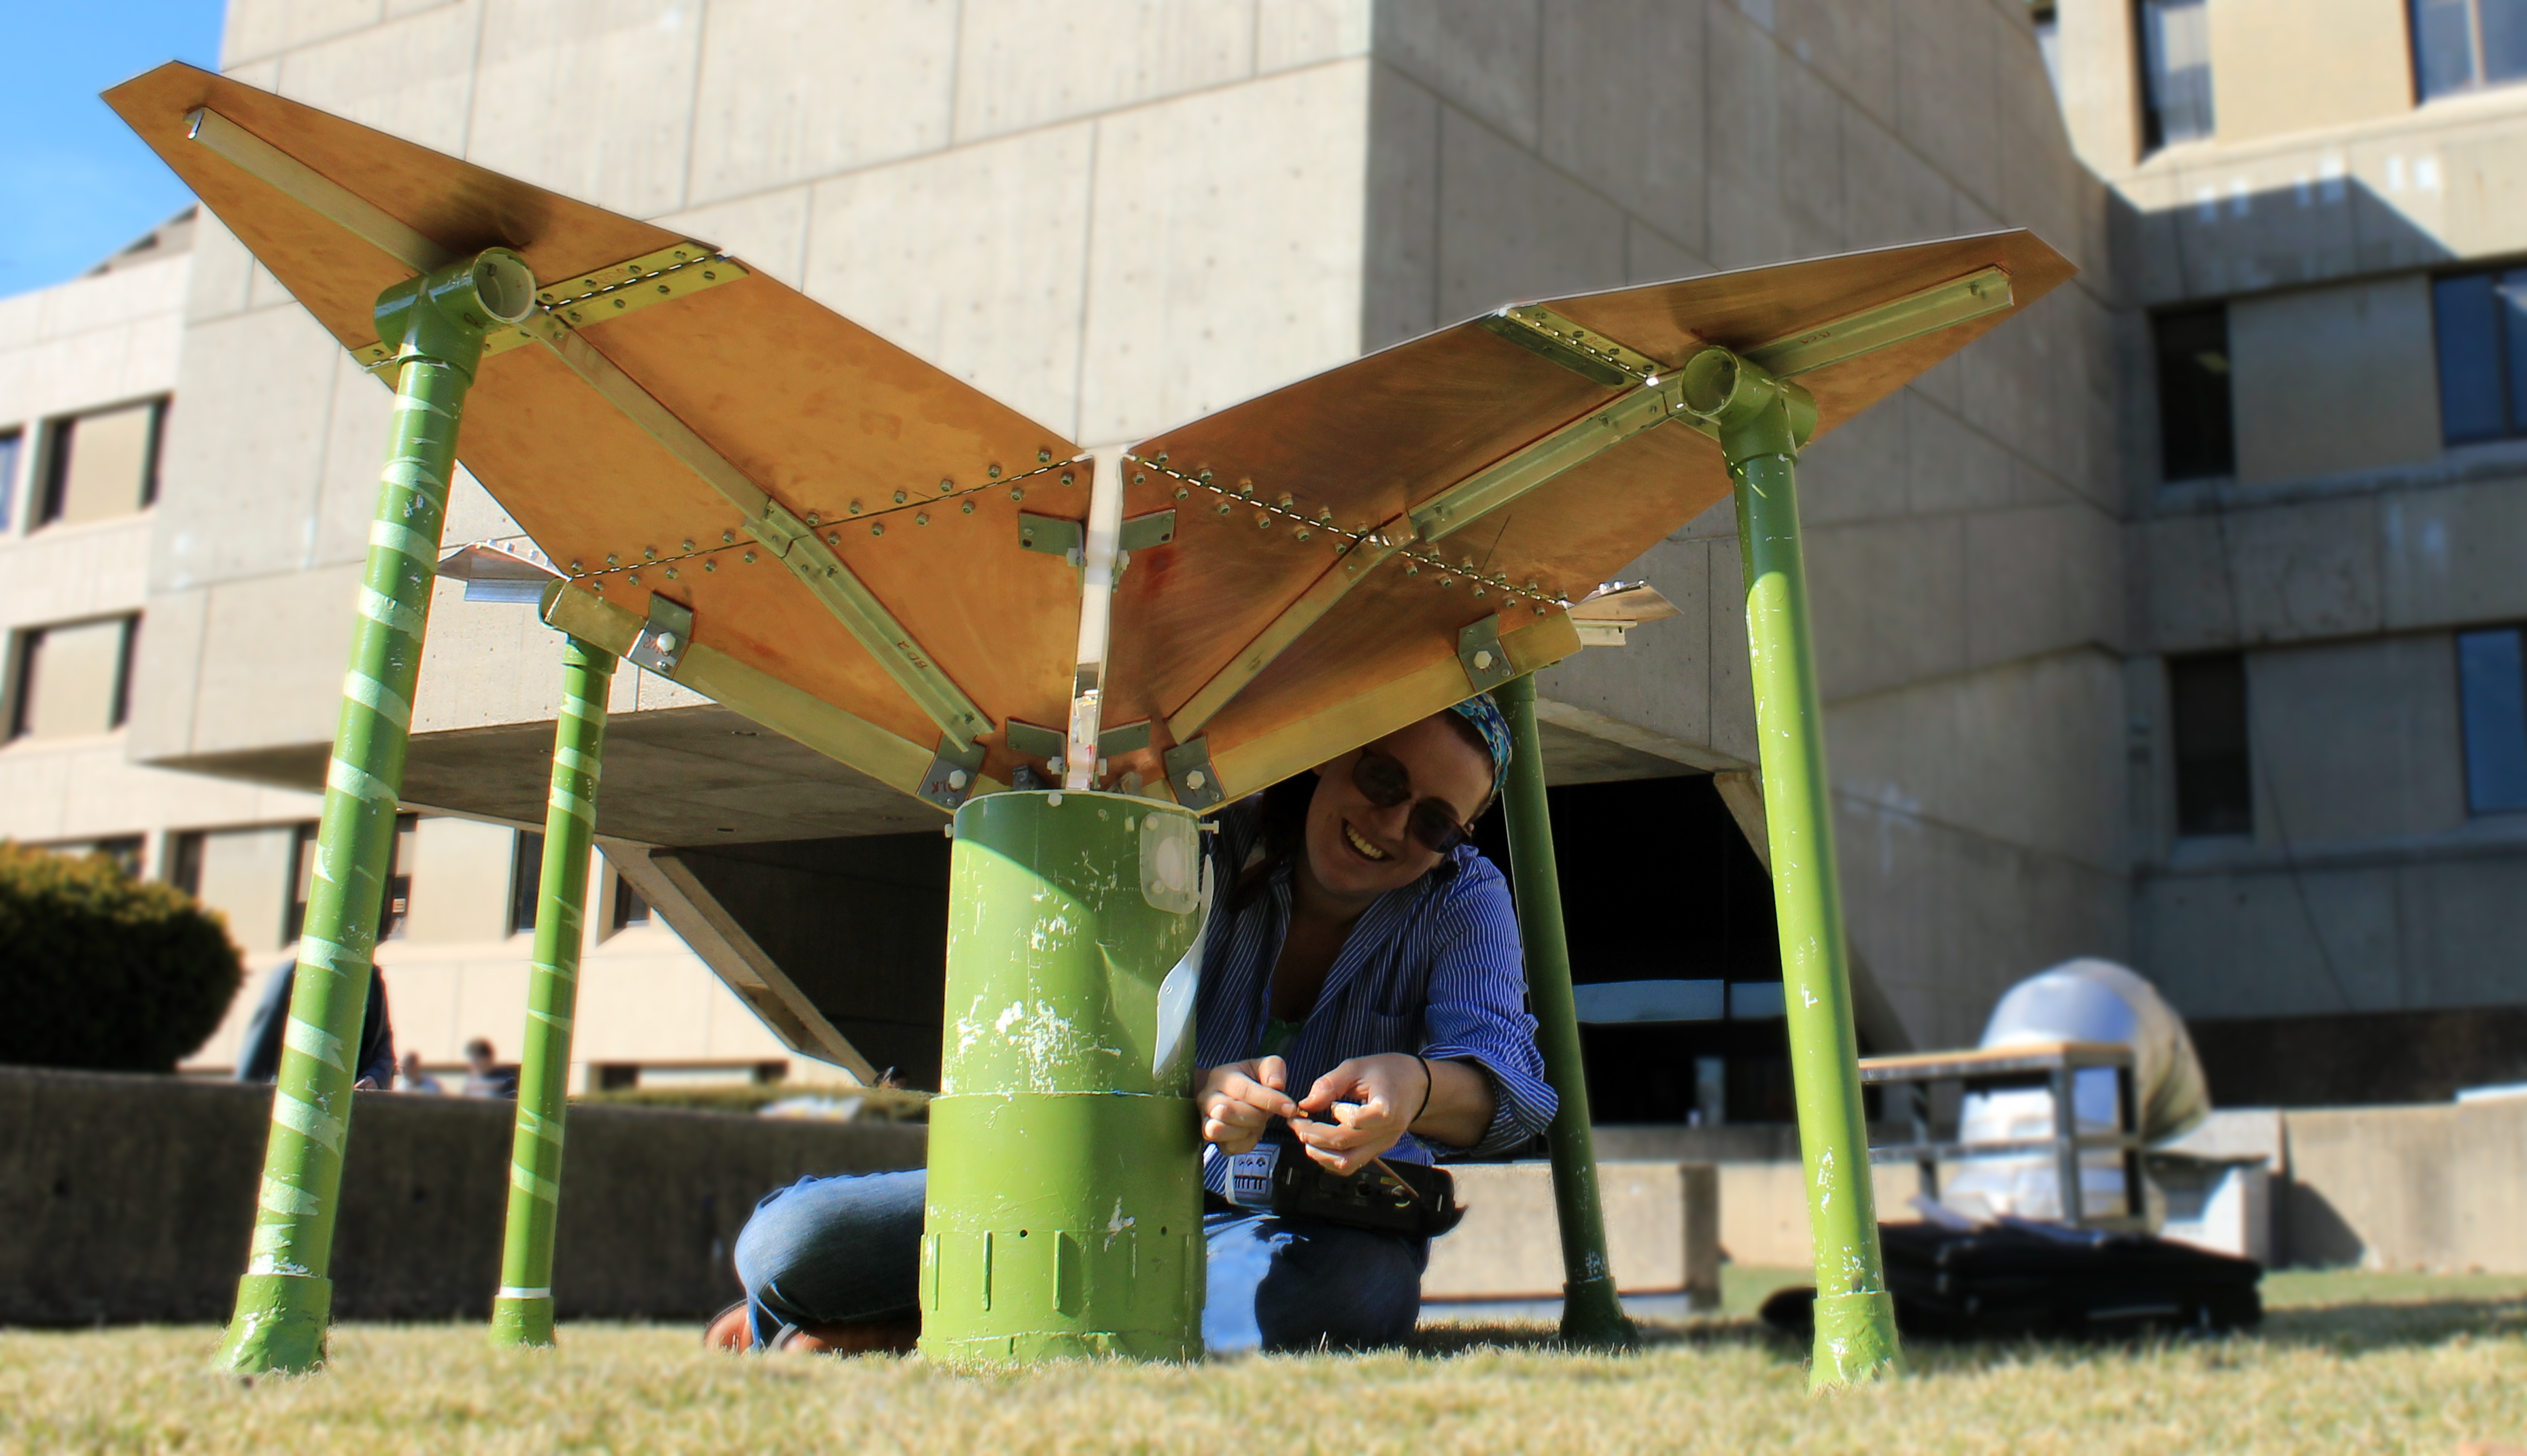
\includegraphics[width=0.95\linewidth]{SCIHI_system/figures/HIbiscus_100mhz.jpg}
\caption{New HIbiscus antenna scaled for 100 MHz as set up on the lawn at CMU while its S-parameters were measured. }
\label{Fig:hibiscus_100}
%\end{minipage}
\end{center}
\end{figure}

\subsubsection{Antenna Upgrades}
Deployment of the SCI-HI system in June 2013 demonstrated that the HIbiscus antenna could use some improvements prior to future deployements. The first and most significant change was the addition of a second antenna scaled to have a center frequency of 100 MHz. By having both scales (70 MHz and 100 MHz), data can now be collected over a wider range of frequencies. In addition, the overlap region where both antennas work ($\sim 85-95$ MHz) provides a cross check for the signal. In other words, this cross check will help us to make sure that any signal measured is not coming from the antenna structure. 

\begin{figure}[htb]
\centering
\begin{minipage}[b]{0.33\textwidth}
\centering
\includegraphics[width=0.95\linewidth]{SCIHI_system/figures/HIbiscus_petals.jpg}
\caption{HIbiscus petals with hinged joints.}
\label{Fig:hibiscus_petal}
\end{minipage}%
\begin{minipage}[b]{0.02\textwidth}
\hspace{1cm}
\end{minipage}%
\begin{minipage}[b]{0.61\textwidth}
\centering
\includegraphics[width=0.95\linewidth]{SCIHI_system/figures/HIbiscus_folded_70mhz.jpg}
\caption{HIbiscus petals folded up in preparation for packing.}
\label{Fig:hibiscus_fold}
\end{minipage}
\end{figure}

We built a new 70 MHz antenna (see Figure \ref{Fig:hibiscus_70}) as well as the 100 MHz antenna (see Figure \ref{Fig:hibiscus_100}) using the same shape as the original antenna. However, our deployment helped us to identify some changes to make to the physical construction of the antenna in order to make it easier to setup. We replaced the brass flanges that had to be screwed together to assemble each petal with hinged joints (made out of piano hinge) that do not have to be disassembled and reassembled (see Figure \ref{Fig:hibiscus_petal}). Figure \ref{Fig:hibiscus_fold} shows two of these petals when they are folded and stacked prior to being placed inside a bag for travel. 

In addition to the hinged joints, we also added extention pieces to the support PVC to allow us to use the same supports for both scaled versions of the antenna. This allowed us to add the second antenna with only one additional bag required for transport of both antennas compared to transport of just the 70 MHz antenna.  

\begin{figure}[htb]
\begin{center}
%\centering
%\begin{minipage}[b]{0.47\textwidth}
%\centering

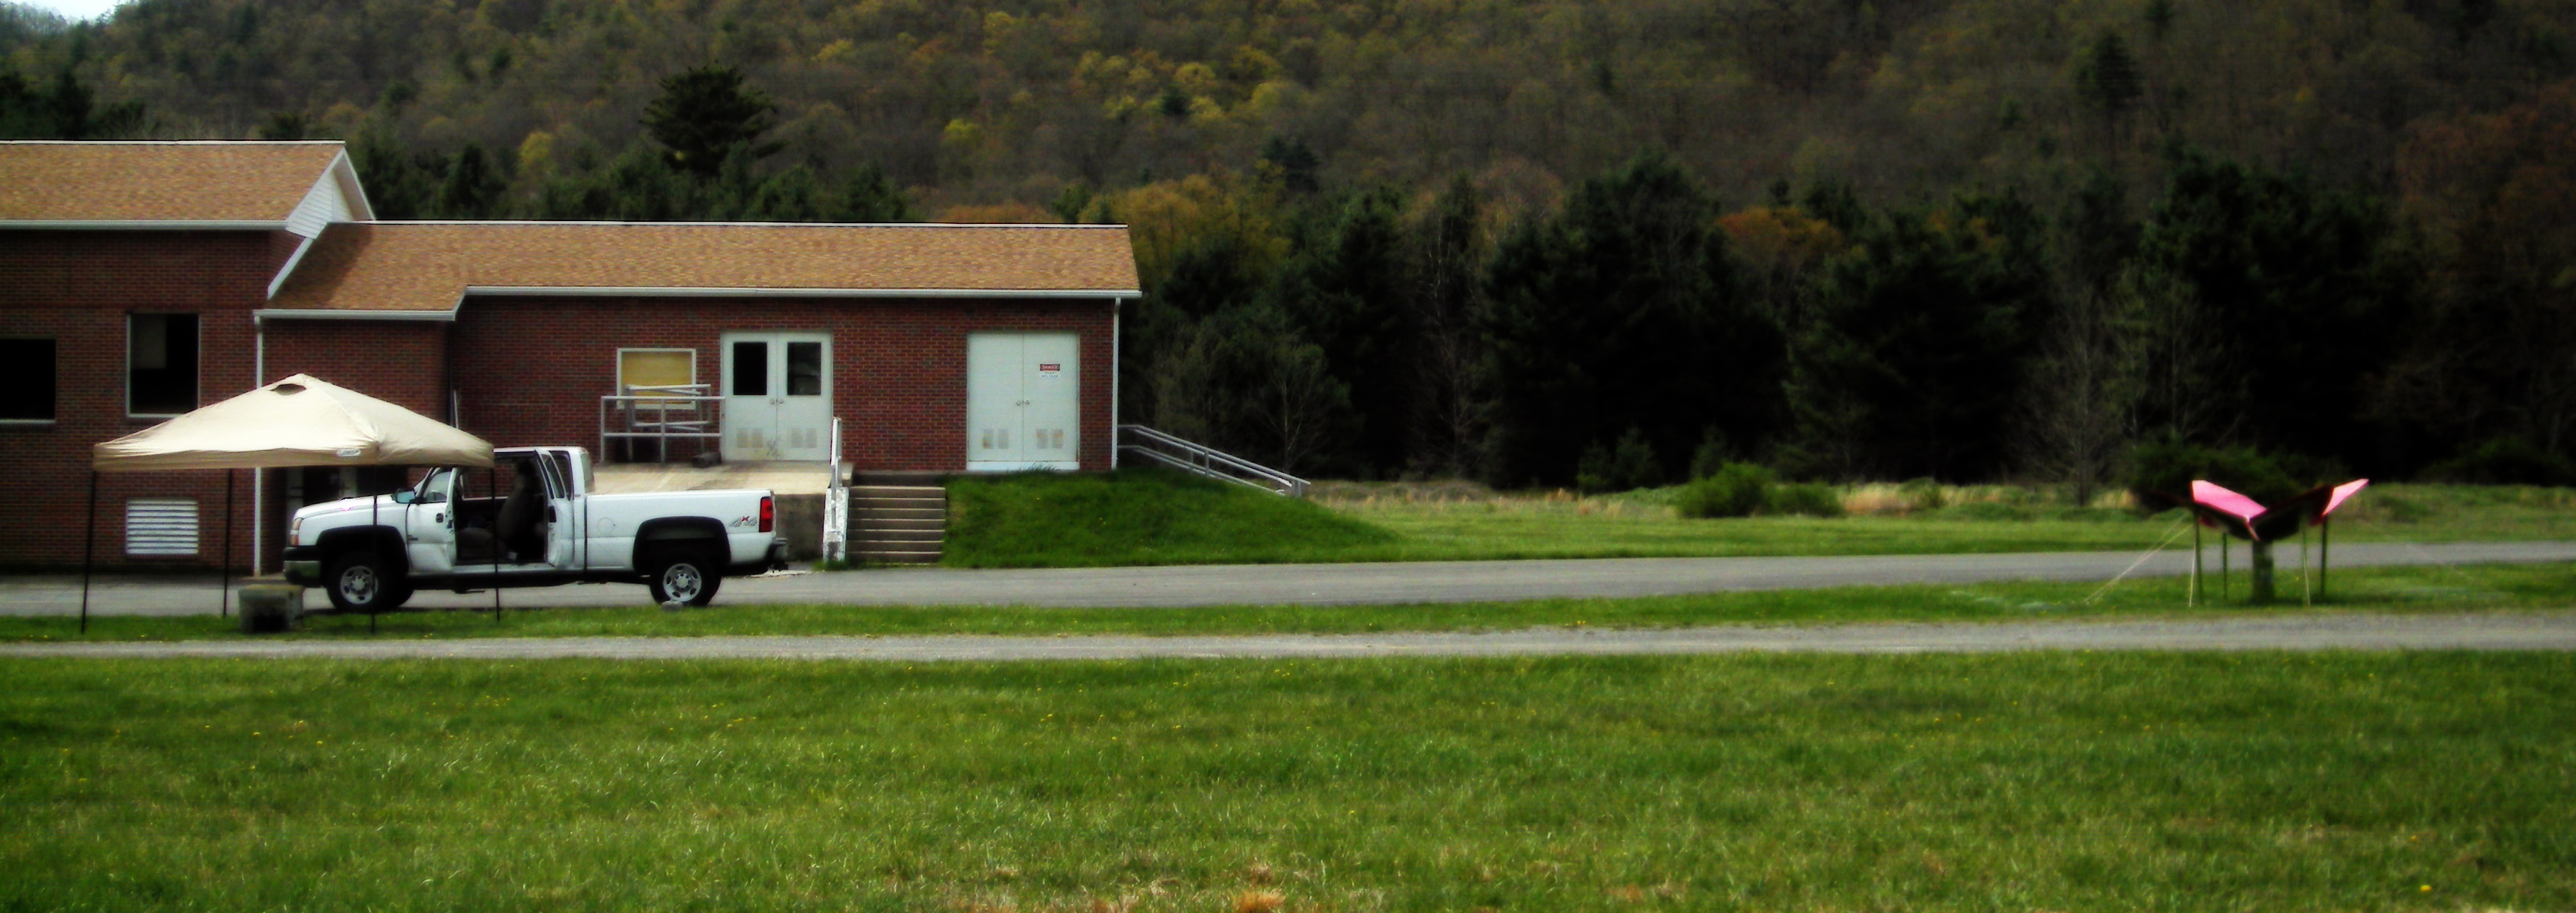
\includegraphics[width=0.95\linewidth]{SCIHI_system/figures/SCIHI_gbt_sys.jpg}
\caption{SCI-HI system with HIbiscus antenna set up on site at Green Bank in May 2013.}
\label{Fig:sys_gbt}

\end{center}
\end{figure}

%\end{minipage}%
%\begin{minipage}[b]{0.02\textwidth}
%\hspace{1cm}
%\end{minipage}%
%\begin{minipage}[b]{0.47\textwidth}
%\centering

\begin{figure}[htb]
\begin{center}
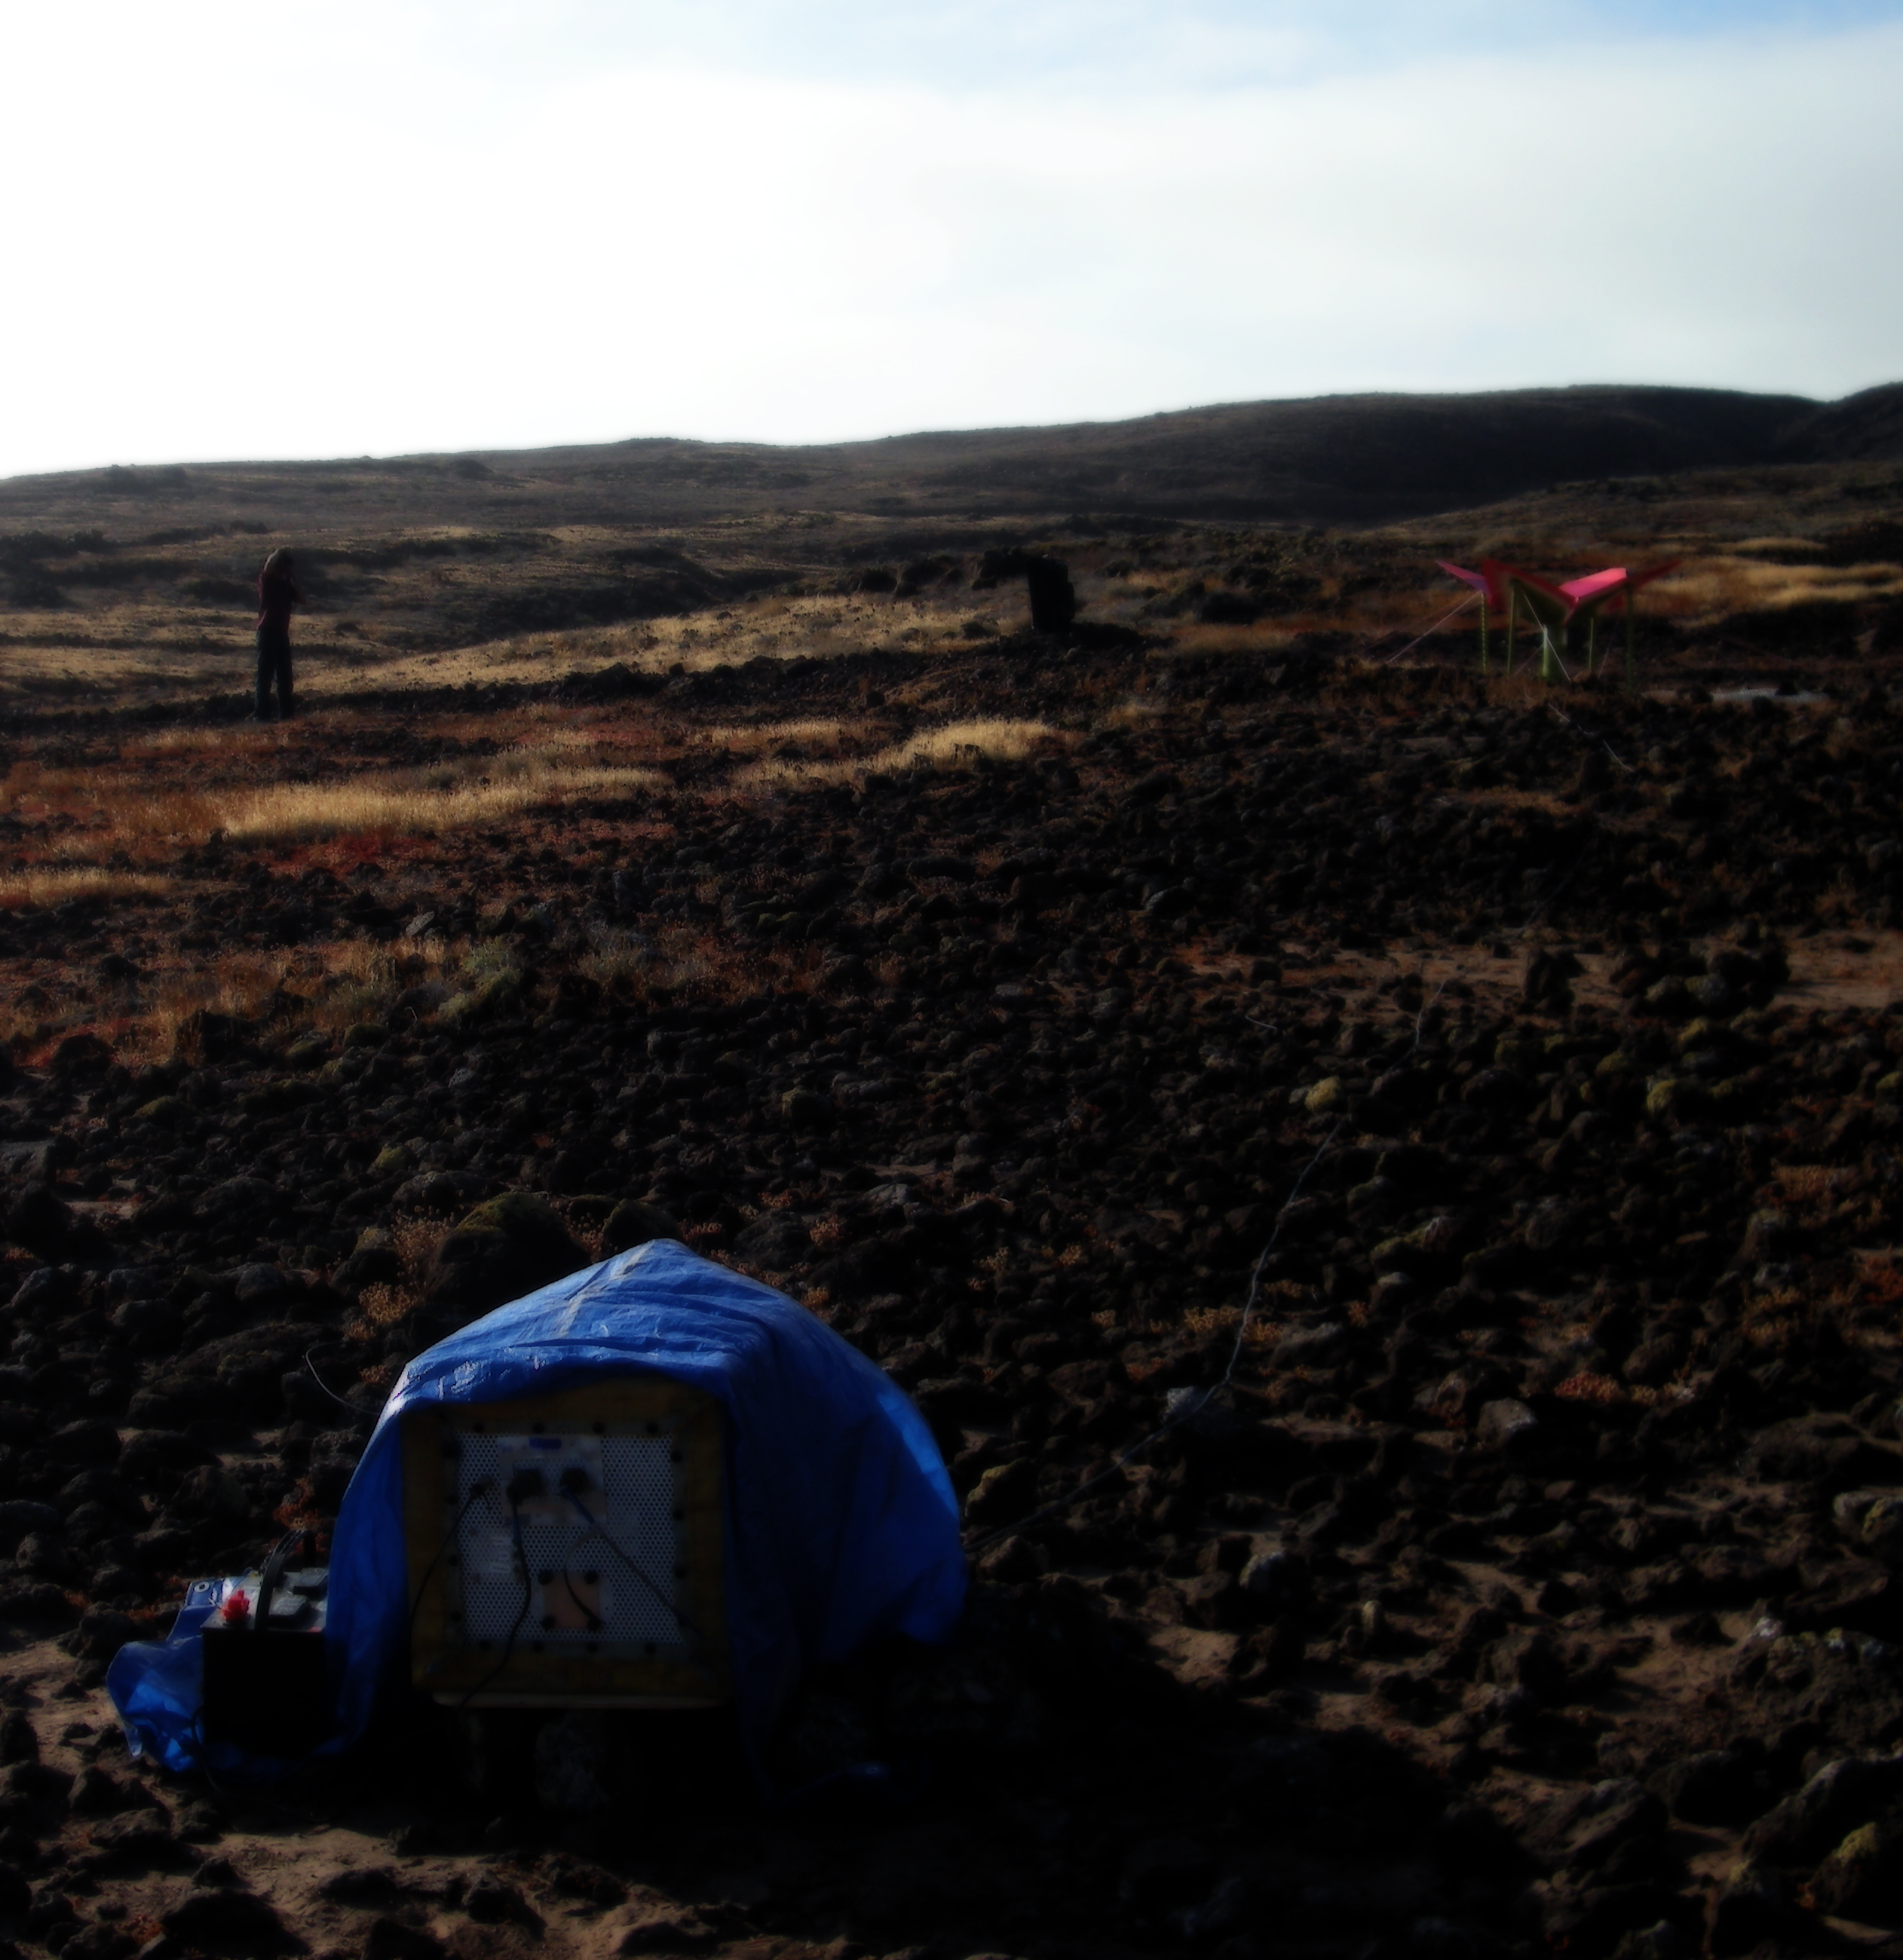
\includegraphics[width=0.85\linewidth]{SCIHI_system/figures/SCIHI_guad_sys.jpg}
\caption{SCI-HI system with HIbiscus antenna set up on site at Isla Guadalupe in June 2013}
\label{Fig:sys_guad}
%\end{minipage}

\end{center}
\end{figure}


\section{RF Electronics}

Once the signal from the sky has been collected by the antenna, it has to be transmitted to the data proccessing system in a form that the system is capable of processing. Transmission happens along a chain of radio frequency (RF) electronics. 

\textcolor{red}{Add a second level RF chain flow chart here.}
\subsection{RF Chain Overview}
For the SCI-HI system, the RF chain components are a switch, amplifiers, high and low pass filters, attenuators and a power splitter (along with the attendant cabling). Each of these components serves a specific purpose in the system. 

We can divide the RF chain into two sections based upon physical location. The first section is the antenna electronics, which sit as close to the antenna terminal as physically possible. The second section is the Faraday cage electronics, which sit next to the data processing system within a Faraday Cage. Between the two sections is a long signal cable ($\sim50-100 m$), allowing the antenna and data processing system to be placed far enough apart that the transmission of self-generated noise from the data processor is minimized (see Figures \ref{Fig:sys_gbt} and \ref{Fig:sys_guad}).

\begin{figure}[htb]
\centering
\begin{minipage}[b]{0.47\textwidth}
\centering
\includegraphics[width=0.95\linewidth]{SCIHI_system/figures/trombone_sys_switch.jpg}
\caption{Trombone antenna setup with calibration switch mounted directly below the antenna.}
\label{Fig:trombone_switch}
\end{minipage}%
\begin{minipage}[b]{0.02\textwidth}
\hspace{1cm}
\end{minipage}%
\begin{minipage}[b]{0.47\textwidth}
\centering
\includegraphics[width=0.95\linewidth]{SCIHI_system/figures/SCIHI_rf_ant_lower.jpg}
\caption{RF electronics box at the base of the trombone antenna with second stage amplifier and filters.}
\label{Fig:trombone_base}
\end{minipage}
\end{figure}

\textcolor{red}{Add a third level RF chain flow chart of just the antenna electronics here.}

\subsection{Antenna Electronics}
The antenna electronics are a calibration switch with known signal sources on some of the terminalsand two stages of amplification. In some versions of the electronics system, at least one of the RF filters was placed at the antenna end of the system but we'll discuss that component in the Faraday Cage electronics section. 

\subsubsection{Calibration Switch}
Because the SCI-HI system has a single antenna with a relatively large beam ($\sim 55^\circ$), calibrating the data from the antenna can be difficult. One way to do this calibration is to use noise source of known temperature whose signal is sent through the same RF chain as the antenna data (see Chapter \ref{Ch:Data}). 

In order to facilitate this calibration, a switch was placed at the terminal of the antenna. By making the antenna one of the inputs of the switch and matching one or more known temperature sources to the other switch inputs, data can be collected for all inputs with the same RF chain. 

We used a 6 input electromechanical switch (\textcolor{red}{Add part numbers here}) for the system. One input to the switch was connected directly to the antenna (see Figures \ref{Fig:trombone_switch} and \ref{Fig:rf_ant_mount}). The other inputs were a short terminator, a $50 \Omega$ load terminatore, a $100 \Omega$ load terminator, and an artificial noise source of known power. One input was left open. 

Switching between inputs is controlled through a cable from the Faraday Cage that carries both the power for the antenna electronics and the control signal. In addtion, the artificial noise source is turned off when that input is not enabled (to avoid noise bleeding into the antenna). We also built a manual switch control box that can be hooked up to the switch for testing. 

\begin{figure}[htb]
\centering
\begin{minipage}[b]{0.47\textwidth}
\centering
\includegraphics[width=0.95\linewidth]{SCIHI_system/figures/SCIHI_rf_ant_box.jpg}
\caption{New lucite box containing all the antenna RF electronics.}
\label{Fig:rf_ant_box}
\end{minipage}%
\begin{minipage}[b]{0.02\textwidth}
\hspace{1cm}
\end{minipage}%
\begin{minipage}[b]{0.47\textwidth}
\centering
\includegraphics[width=0.95\linewidth]{SCIHI_system/figures/SCIHI_rf_ant_box_mount.jpg}
\caption{RF electronics box attached to one of the HIbiscus antenna center mounts.}
\label{Fig:rf_ant_mount}
\end{minipage}
\end{figure}

\subsubsection{Amplifiers}
Immediatelly following the switch in the RF chain is the first stage amplifier. 

\textcolor{red}{Add general discussion of S-parameters and Transmission Efficiency followed by a section on the different types of amplifiers that we tried and why we selected the one that we did.}

\paragraph{S-parameters}

\paragraph{Transmission Efficiency}

\paragraph{Amplifier Selection}

\paragraph{Multi-stage Amplification}
Because the $\sim50-100 m$ signal cable will attenuate signals travelling down its length, a second stage amplifier was added to the system to increase the gain of the signal. Both amplifiers use DC power supplied by the same power cable as the switch. Because different levels of DC power were needed for the varying electronic components, voltage regulation circuits were also included in the antenna electronics housing. 

To maintain transmission efficiency, the first and second stage amplifiers' impedence had to match well. This was accomplished by using the same amplifier type for both stages. Initially the second stage amplifier was placed at the base of antenna (see Figure \ref{Fig:trombone_base}). However, this placement resulted in reflections in the signal whose period corresponded to the cable length between the two amplifiers. \textcolor{red}{May try to make a plot that shows this.} Therefore, the second stage amplifier was moved to a position immediately following the first stage amplifier (see Figure \ref{Fig:rf_ant_box}), which removed the effect. The total gain of the amplifiers was $\sim$50 dB over the entire frequency band. 

\textcolor{red}{Add a third level RF chain flow chart of just the Faraday cage electronics here.}

\subsection{Faraday Cage Electronics}
Once the signal has travelled down a long cable from the antenna, there are a few electronic stages that it must pass through prior to entering the data processing system. A third stage amplifier is needed to compensate for the attenuation caused by the long cable, filters are needed to keep signals from outside the frequency band of interest from overloading the data processing system, and a signals splitter used to achieve the necessary data sampling rate. All of these electronics, as well as the data processing system, were placed inside a Faraday cage designed specifically to accomodate them. 

\begin{figure}[htb]
\centering
\begin{minipage}[b]{0.36\textwidth}
\centering
\includegraphics[width=0.95\linewidth]{SCIHI_system/figures/SCIHI_fcage_old.jpg}
\caption{Faraday cage around data processing system as setup in October 2012.}
\label{Fig:fcage_old}
\end{minipage}%
\begin{minipage}[b]{0.02\textwidth}
\hspace{1cm}
\end{minipage}%
\begin{minipage}[b]{0.58\textwidth}
\centering
\includegraphics[width=0.95\linewidth]{SCIHI_system/figures/SCIHI_filter.jpg}
\caption{System power and control signal filter box for one of the Faraday Cages.}
\label{Fig:fcage_filter}
\end{minipage}
\end{figure}

\subsubsection{Faraday Cage Design}
The design of the Faraday Cage for the SCI-HI system was inspired by the dual requirements of space and portability. Because the wavelengths being studied with the system are $\geq 2$ meters, metal mesh could be used in place of solid metal for the sides of the cage. This mesh is considerably lighter than solid metal, but does not hold its structure. So I came up with a design that uses a metal mesh bag with a PVC pipe framework placed inside to hold its shape (see Figure \ref{Fig:fcage_old}). The mesh bag folds up like a paper bag and the PVC framework can be disassembled, allowing it to be packed up into a suitcase. 

Access to the Faraday cage was supplied through the front panel, which attached to the rest of the bag through a set of metal snaps spaced less than 20 cm apart. This front panel included access ports for the signal cable, as well as the power and switch control cable. Multiple versions of the Faraday cage were constructed, but all of them used the same mesh bag system (see Figures \ref{Fig:fcage_int} and \ref{Fig:fcage_new}). 

\begin{figure}[htb]
\centering
\begin{minipage}[b]{0.44\textwidth}
\centering
\includegraphics[width=0.95\linewidth]{SCIHI_system/figures/SCIHI_fcage_int.jpg}
\caption{Faraday cage around data processing system as setup in June 2013.}
\label{Fig:fcage_int}
\end{minipage}%
\begin{minipage}[b]{0.02\textwidth}
\hspace{1cm}
\end{minipage}%
\begin{minipage}[b]{0.50\textwidth}
\centering
\includegraphics[width=0.95\linewidth]{SCIHI_system/figures/SCIHI_fcage_new.jpg}
\caption{Faraday Cage with double shielding around data processing system, currently under development.}
\label{Fig:fcage_new}
\end{minipage}
\end{figure}

\subsubsection{Power Filters}
Because the power and switch control cable carried DC power out to the antenna electronics, it needed to be filtered to keep RF signals from using the cable to escape the Faraday Cage. To accomplish this, a set of filter boxes were placed in the DC power and switch control signal lines. These filter boxes (see Figure \ref{Fig:fcage_filter}) were low pass filters with over 40 dB of attenuation at 40 MHz. Two stages of filtering were included to ensure that there was no signal transmission through the DC power lines. 

Once the battery was placed outside of the Faraday Cage, filters also had to be used between the battery and the electronics inside the cage. The same filters used for the DC power and switch control cable were also used to make sure that RF signals didn't use the power supply cable from the battery to transmit outside the Faraday Cage.  


\subsubsection{System Power} \label{Sec:sys_power}
The entire system was powered using deep-cycle automotive batteries. These batteries supplied 12 V unregulated power, which was used by both the data processing system and the RF electronics. Initial designs of the Faraday cage had the DC battery stored inside the Faraday Cage, as shown in Figure \ref{Fig:fcage_old}. Later, the battery was moved outside the cage for easier access (see Figure \ref{Fig:fcage_int}). A fully charged battery could power the entire system for $\sim$12-15 hours. 

Charging batteries was a big part of the support process for the SCI-HI system. Keeping the system running continually required at least 3 batteries with regular access to a battery charger and transport between the SCI-HI site and the battery charging location 2-3 times a day. 

An alternative to running off batteries is to use a small portable gasoline or diesel generator. Using this generator would cut down on the number of site visits required, as the generator would run constantly with only occasional stops to top off the fuel. However, using a generator also provides a new source of RF noise (particularly a gasoline generator with spark plugs). Placing the generator inside its own Faraday Cage should attenuate this noise, but it is a factor that must be accounted for in selecting a power source. 

\subsubsection{RF Filters and Amplification}
Once the signal from the antenna entered the Faraday Cage, the first part of the RF chain was a set of filters. These filters were a low pass filter at 200 MHz (\textcolor{red}{add part number here}) and a high pass filter at 30 MHz (\textcolor{red}{add part number here}). The low pass filter was placed to prevent signals from higher frequencies ($\geq 200$ MHz) from aliasing into the frequency range where we were observing. The high pass filter was placed to prevent signals from the AM band and below overloading the sampling system, which could affect the overall system gain or create spurious signals in the observing band. 

After the signal has passed through the long cable and the filters, it is necessary to add another level of amplification to the system. This final stage of amplification is to bring the signal levels to a point where they can be clearly distinguished from system noise by the data processing system and adds $\sim25$ dB of gain. The amplifier used here is a \textcolor{red}{Add part number here} minicircuits amplifier, which is supplied with regulated power from the DC source. 

\subsubsection{RF Signal Splitting} \label{Sec:hard_split}
The analog to digital conversion (ADC) card used in the data processing system is limited to a 250 MSamples-per-sec sampling rate, but the bandwidth of the system is over 125 MHz. In order to expand the operating range of the ADC, a hardware $''$trick$''$ is used.

The signal from the antenna is split into two identical signals with a \textcolor{red}{Add part number here} splitter. Both signals are then sent to the ADC using two of the input ports. However, the lengths of the cables placed between the two outputs of the splitter and the two input ports of the ADC are slightly different. The difference (\textcolor{red}{Add exact length here} is exactly matched such that a sample taken from one input port is has been delayed by 2 ns compared to the other input port. If the signals from both ports are combined, the data now appears to have been sampled at 500 MSamples-per-sec. 


\section{Data Processing System}

\subsection{Data Processing Pathway}
As discussed in Section \ref{Sec:hard_split}, signals from the sky enter the system via two ports of an analog to digital conversion (ADC) card. For the SCI-HI system, we used a \textcolor{red}{add part name and number here} card. Data is collected for one second of integration, with the interleaving stragegy producing 500 MSamples of data. 

Storing the entire dataset for each second would require a great deal of space. Instead, a fast fourier transform (FFT) is performed on the dataset. The frequency spectrum produced by the FFT takes up much less space (\textcolor{red}{How much less?}) and is stored by the system. The process is then repeated for another second of data. 

Because of the design of the system, collecting new data can only be done after the FFT is complete. This means that the system is less than 100\% efficient, or it takes longer than 1 second to record the frequency spectrum of 1 second of data. Initially the FFT calculation was quite time consuming ($\sim 30-60$ seconds), but improvements to the software and hardware have decreased this calculation rate to $\sim 2$ seconds. This means that the system has a maximum duty cycle of $\sim30$\%. 

All of the frequency spectrum data is stored locally on the hard drive of the processing system. The relatively small data volume ($\sim 2$ Gb per day) means that data transfer can be done using small USB drives. During deployment, data was removed from the hard drive 2-3 times a day and stored locally on multiple laptop computers and external hard drives before being uploaded to a server upon return to $''$civilization$''$. 

\subsection{System Control and User Interface}
In addition to the data processing software, a graphical user interface was designed for diagnostic and control purposes. This interface displays the most recent frequency spectrum collected by the system and lets the user set the current data collection mode (including switch control). The user can choose to either take a single data set with any of the switch positions (Antenna, 50 $\Omega$, Short, Noise Source, 100 $\Omega$), or take continual data with a set number of Antenna datasets followed by a single dataset from each of the calibration sources. \textcolor{red}{Add screenshot of the UI here}

The system default upon start-up is to run in continual data collection mode with the number of antenna iterations as set by the system when it was previously used. To lower the power consumption and space requirements of the system, it is designed to be run without a monitor, mouse and keyboard. Instead, the system can be controlled by an external system through an ethernet port. This port is only used when the system needs to be checked.

\subsection{Control Computer}
The data processing system can be diagnosed using a personal computer (such as a laptop) with an ethernet port. However, an additional diagnostic computer was also developed for the SCI-HI system. This computer is a Raspberry Pi\footnote{www.raspberrypi.org} with a small monitor, mouse and ethernet port. \textcolor{red}{Add picture of the diagnostic computer.} Using this small computer, we can quickly check that the system is working properly and run simple diagnostics.

\subsection{Power Suppy and Consumption}
In order to power the data processing system, a computer power supply had to be selected that matched the system power source (DC battery). Initially, we started with a typical AC computer power supply and a DC to AC inverter that converted the incoming DC power from the batteries into AC power that the computer could handle. 

While using an inverter is the simplest solution, it is very energy inefficient.  \textcolor{red}{Add exact inefficiency of the inverter we were using in percentages.} Additionally, any failure of the inverter can crash the entire system. Therefore, we decided to switch to an entirely DC system by replacing the AC power supply for the computer with a power supply that takes input DC power. \textcolor{red}{Add original DC power supply part number here.} 

Utilizing this power supply greatly lowered our power consumption. However, we found that the power supply we selected was not reliable. Most of the DC power supplies on the market are designed for automotive applications, where they are only needed for short durations rather than continual use. In particular, the DC power supply was particularly unhappy when running in a low battery situation. We are currently exploring different alternatives, as discussed in Section \ref{Sec:sys_power}. 

\begin{figure}[htb]
\centering
\begin{minipage}[b]{0.52\textwidth}
\centering
\includegraphics[width=0.95\linewidth]{SCIHI_system/figures/SCIHI_comp.jpg}
\caption{Current version of the data processing system assembled inside a Faraday Cage box.}
\label{Fig:new_comp}
\end{minipage}%
\begin{minipage}[b]{0.02\textwidth}
\hspace{1cm}
\end{minipage}%
\begin{minipage}[b]{0.42\textwidth}
\centering
\includegraphics[width=0.95\linewidth]{SCIHI_system/figures/SCIHI_water_cooling_pipe.jpg}
\caption{Part of the water cooling system for the data processing machine.}
\label{Fig:water_pipe}
\end{minipage}
\end{figure}

\subsection{System Noise Generation}
Deployment to Isla Guadalupe in June 2013 indicated that our Faraday Cage design had insufficient attenuation of self-generated RFI from the data processing system. This problem was not identified until deployment at the site due to the low levels of RFI compared to external RFI at the testing locations. Self-generated RFI was particularly noticeable above 90 MHz, (see Figure \textcolor{red}{Add time average plot here})but may be present in the data in the lower frequencies as well. Our data indicated that the strength of the self-generated RFI was correlated with the voltage (or charge level) of the DC batteries (see Figure \textcolor{red}{Add waterfall plot here.}). 

In order to address this problem, a more robust Faraday Cage was designed for the SCI-HI system. This Faraday Cage is a double layer cage (see Figure \ref{Fig:new_comp}) with the data processing system placed inside a solid aluminum sealed box and a second Faraday cage with the rest of the electronics placed around the inner box. 

Using a set of two walkie talkies, the aluminum box was tested to show attenuation $\geq$70 dB before modification. This was measured by placing one walkie talkie inside the box in recieve mode and transmitting a signal with the other walkie talkie. If the attenuation was smaller than the transmitted signal, then the recieving signal would make a noise. Even transmitting from less than 1 meter from the box, the signal was not picked up by the reciever. 

However, the problem with using a solid metal Faraday Cage is that it becomes very difficult to cool the system. we designed a water cooling system using copper tubing mounted to the inside of the box (see Figure \ref{Fig:water_pipe}) and heat fins mounted to the outside of the box. A fan with its own Faraday cage was also mounted to the outside of the box to aid heat transfer. This system has been found sufficient for cooling in lab tests, but has not yet been tested in the field. 

\section{Summary}

\textcolor{red}{Should I put something here, and if so, what?}

\chapter{Radio Frequency Interference (RFI) and Site Testing} \label{Ch:RFI}

\section{Overview}

One of the challenges of radio astronomy is locating observing sites that meet the environmental, atmospheric, and ionospheric requirements of a particular set of observations. Potential sites must be assessed for their viability prior to significant experiment development and observation at those sites. Site assessment must include four elements, each of which must be addressed to evaluate the site quality. 

First, does the site have any nearby man-made sources of time independent or continual radio frequency interference (RFI) in the frequency band of the observations? Initial evaluation of this requirement can be done using a simple broadband antenna and spectrum analyzer on site at multiple locations. Deployment of an identical system at different sites allows a much more reliable comparison than can be made with independent systems. 

Second, is the site logistically accessible for the type of equipment needed for a set of observations? Some important considerations include the availability of power, roads or other transport into/out of the location, housing and other observer requirements and site access permissions (such as permits). Assessment of these considerations often requires an in-person visit and an ongoing relationship with the agencies controlling the site.

Third, are there atmospheric effects that must be considered in assessing the viability of a site (e.g. contributions of meteor scatter, thickness of ionosphere, inclement weather)? Tracking data may be available from external sources such weather surveys, but it is often limited to broad trends instead of local details. 

Fourth, are there sources of time variable RFI visible from the site? This can be more difficult to evaluate as it requires a long period of data collection. In cases where time-variable RFI is expected to play a significant role in the data collection, semi-permanent systems may need to be installed to track the RFI environment over time. 

In the following sections, I will evaluate both existing telescope sites and new sites based upon the requirements listed above. Using data collected in Pittsburgh, Pennsylvania, which as a major metropolitan area is not expected to be a suitable radio astronomy site, I will demonstrate the site testing system. I will then look at several existing radio telescope sites and examine their strengths and weaknesses. Finally, I will report on several new radio sites, comparing them to the existing sites to demonstrate viability. 


\begin{figure}[htb]
\centering
\begin{minipage}[b]{0.47\textwidth}
\centering
\includegraphics[width=0.95\linewidth]{RFI_testing/figures/site_testing_kit.jpg}
\caption{Site testing kit laid out in the lab (portable Spectrum Analyzer in inset).}
\label{Fig:site_kit}
\end{minipage}%
\begin{minipage}[b]{0.02\textwidth}
\hspace{1cm}
\end{minipage}%
\begin{minipage}[b]{0.47\textwidth}
\centering
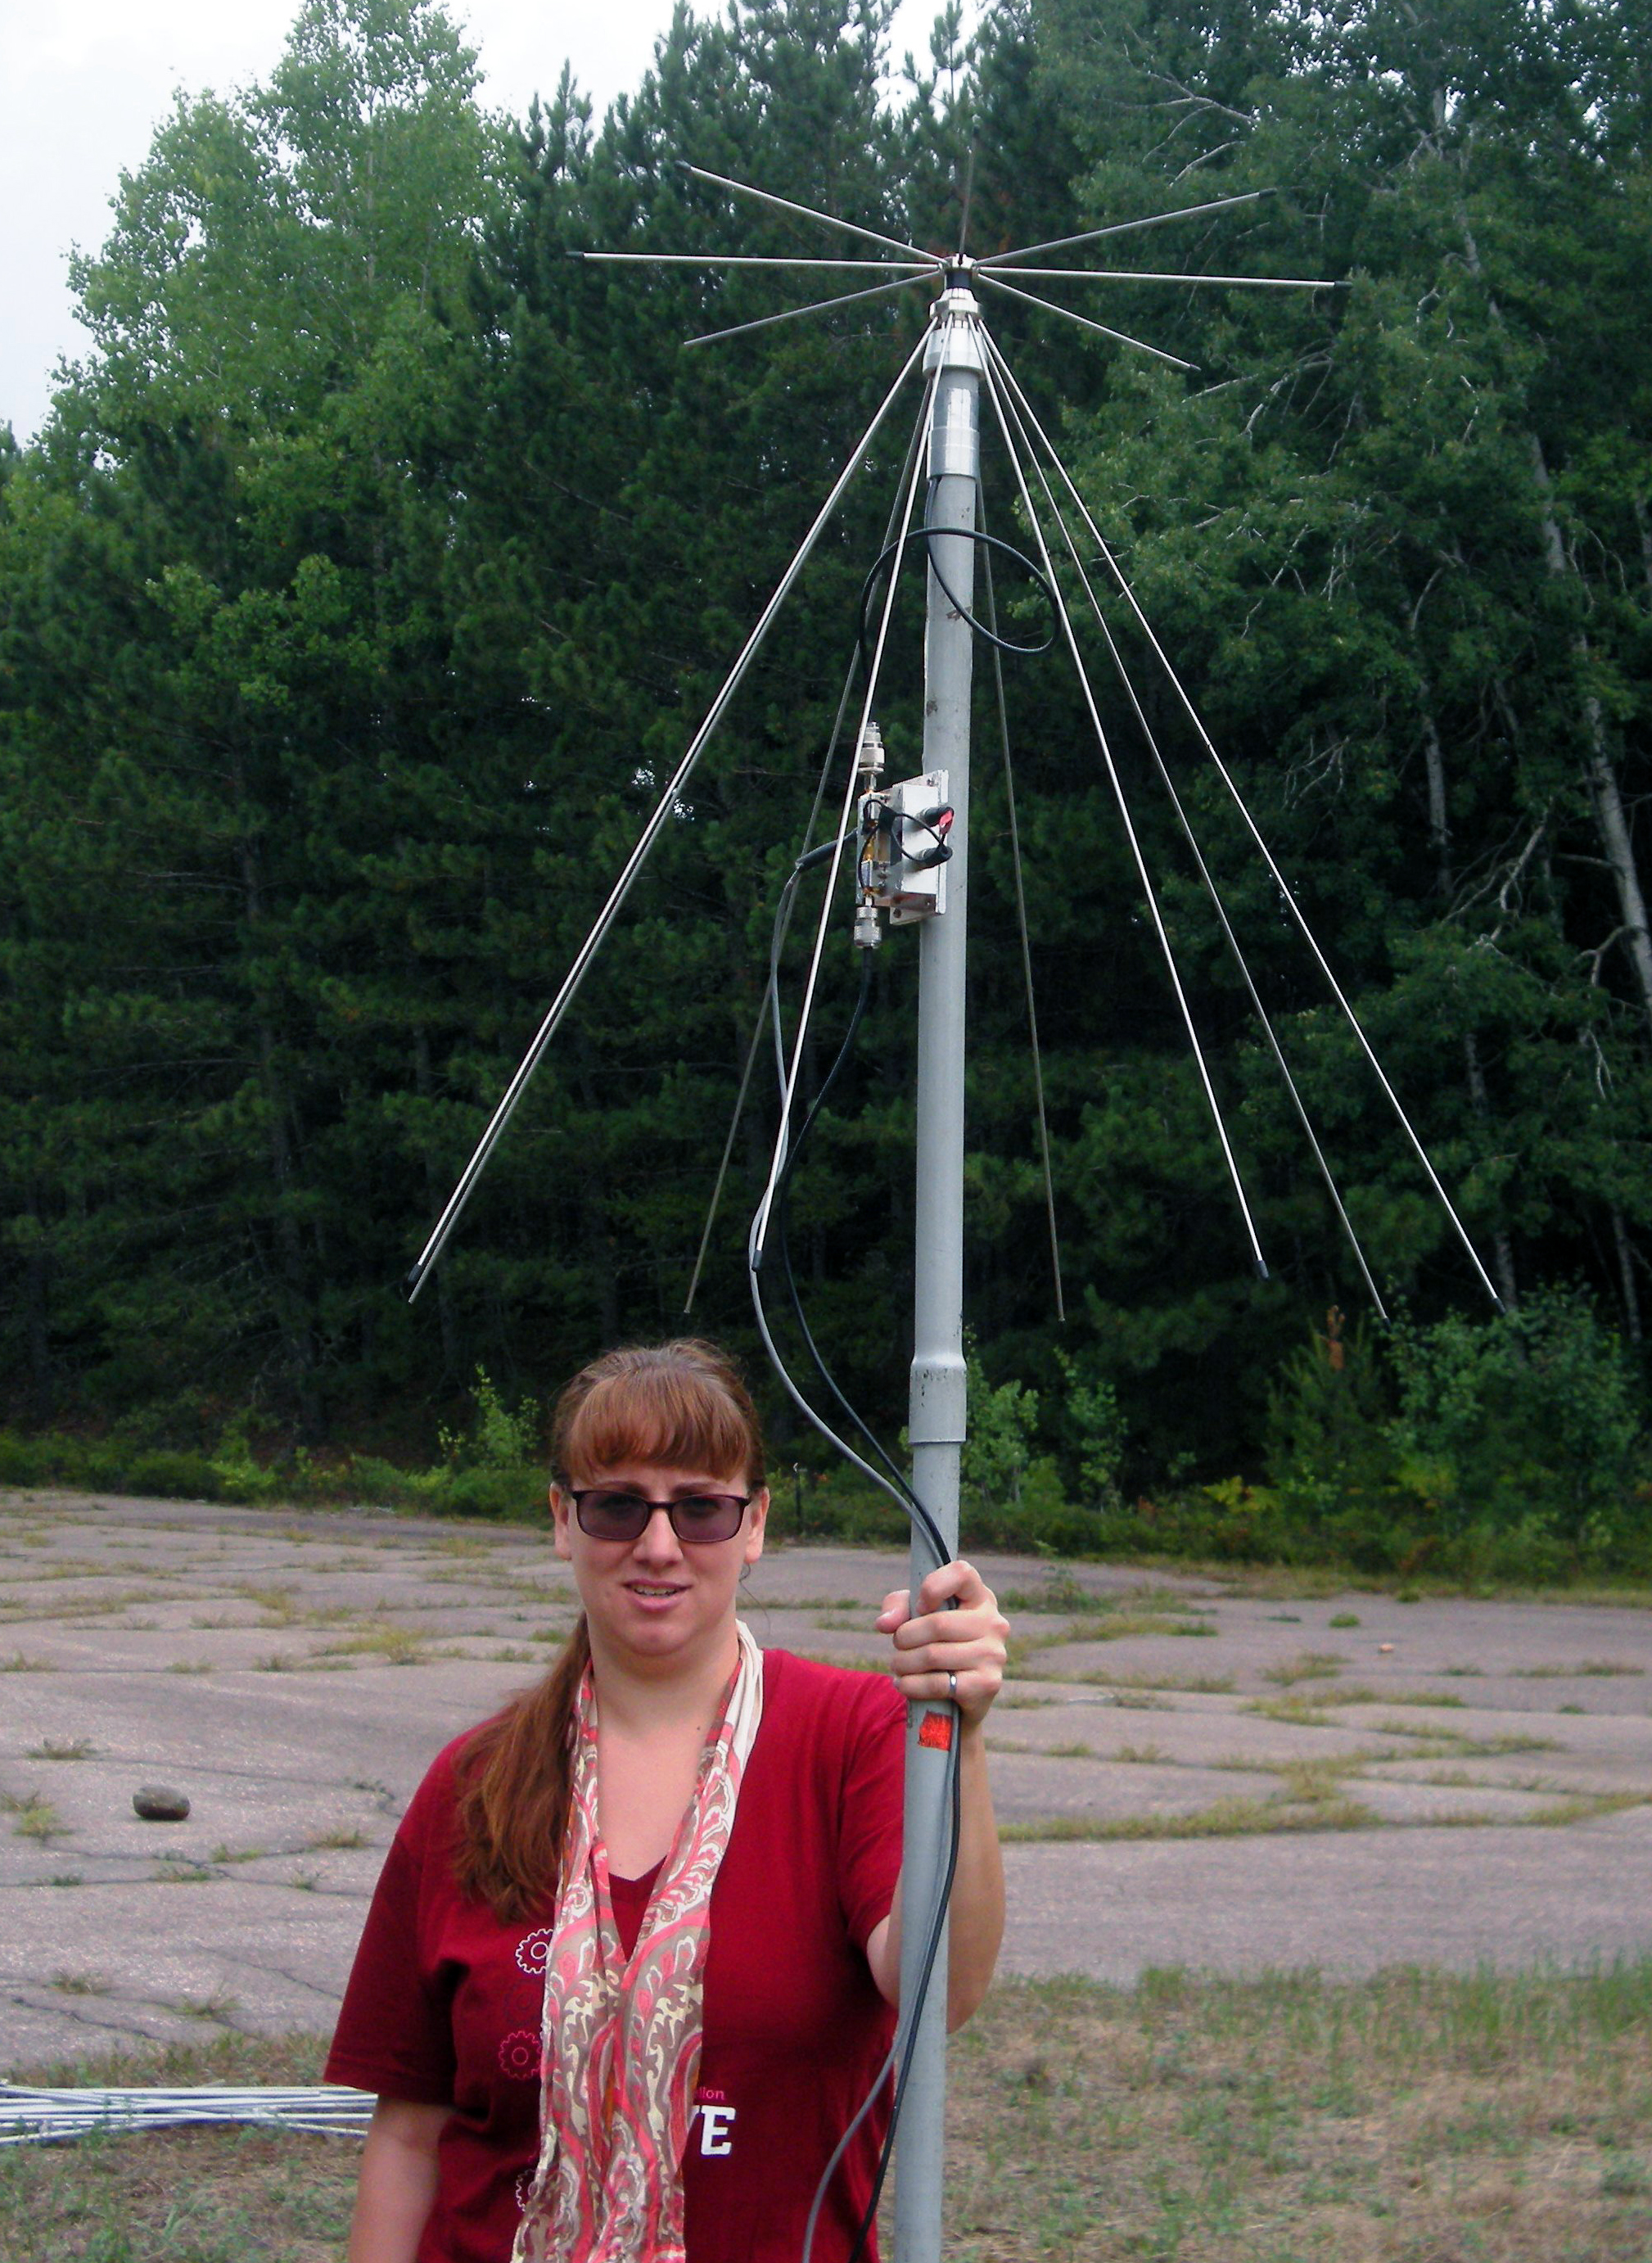
\includegraphics[width=0.95\linewidth]{RFI_testing/figures/voytek_site_test_alg.jpg}
\caption{Tabitha collecting RFI data with the site testing equipment while at one of the testing sites.}
\label{Fig:aroant}
\end{minipage}
\end{figure}

\begin{figure}[htb]
\begin{center}
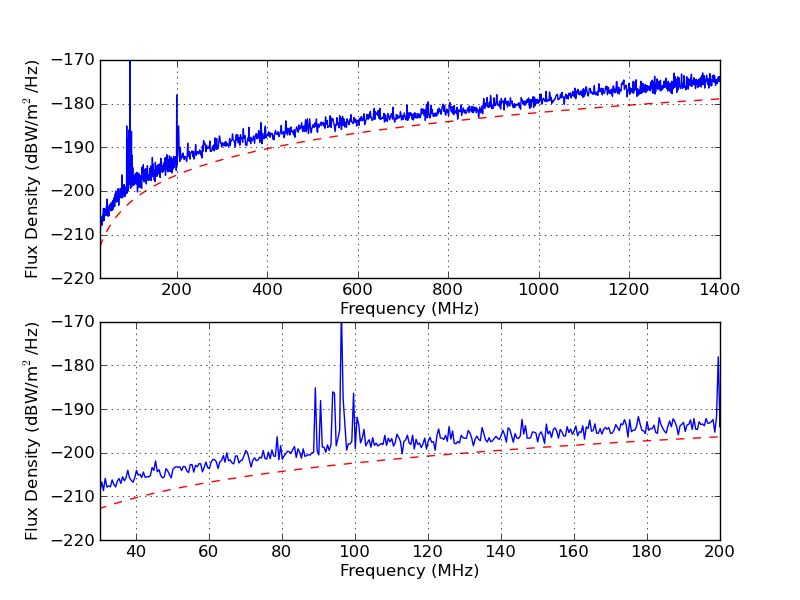
\includegraphics[width=0.9\linewidth]{RFI_testing/figures/50Ohm_cal.png}
\caption{Resistor measurement with the site testing kit. Blue line shows measured power from a $50 \Omega$ resistor. In the data, FM spikes are RF leakage due to the measurement being made in the lab in Pittsburgh where the FM band is extremely loud. Meanwhile, the red line is the expected signal level of a $50 \Omega$ resistor based on Equation \ref{eq:resflux}. The difference between the expected signal and actual signal can be attributed to limitations of the Spectrum Analyzer in measuring flux density.}
\label{Fig:resflux}
\end{center}
\end{figure}

\subsection{Site Testing Kit} \label{Sec:site_kit}

One major element of site evaluations was a set of single time sweep measurements of the RFI over a wide frequency band at each site. To do this, a site testing kit was assembled. The kit includes a broadband antenna, amplifiers, and a portable Spectrum Analyzer for data collection. 

RFI signals are received by the antenna and passed along the RF electronics into the Spectrum Analyzer. RFI is first received by the antenna, a Workman $T-601$ discone antenna with a vertical polarization and a 3 $m$ PVC pipe mast (see Figure \ref{Fig:aroant}). From the antenna, the received signal is then sent through a $50$ $cm$ cable to a set of amplifiers powered by a DC battery pack. The amplifiers are Minicircuits $ZX60-33LN$ followed by Minicircuits $ZX60-4016E$. The signal is then sent down a $\sim 7$ $m$ cable to the Spectrum Analyzer. The Spectrum Analyzer (Anritsu $MS2711A$) was enclosed in a brass mesh bag (Faraday Cage) to minimize self-generated RF contamination. 

Data is collected by sweeping individual $200 MHz$ bands from $\sim1 MHz$ to $1600 MHz$, with a video and resolution bandwidth of $100 kHz$. Only 400 data points are saved by the Spectrum Analyzer, requiring the data to be rebinned down to $500 kHz$ resolution. The highest peak of the $\sim50$ data points within each $500 kHz$ band is stored, which can be accounted for by changing the resolution bandwidth to an effective bandwidth of $30 kHz$. 

In order to convert the data to flux density (S in $dB \; W/m^2Hz$), Equation \ref{eq:fluxdens} was applied to the data. In the equation, $G$ is the amplifier gain in dB, $BW$ is the effective spectrum analyzer bandwidth in $Hz$ and $G_{ant}$ is the antenna gain in dB. 

\begin{equation}\label{eq:fluxdens}
S \Bigg( \frac{dB \; W}{m^2 Hz} \Bigg) = P_{meas} (dBm) - 30 \Bigg( \frac{dB \; W}{dB \;m} \Bigg) - G - 10log_{10} [BW] - G_{ant}
\end{equation}

Amplifier gain ($G$) was measured in the lab using a noise figure meter and antenna gain ($G_{ant}$) can be calulated using Equation \ref{eq:gant}, where $\nu$ is the frequency in $Hz$, and $A_g$ is the isotropic antenna gain in $m^2$. We used a value for $A_g$ corresponding to the typical value for our antenna, which is $1 dB \;i$ or $10^{1dB \;i/10} m^2$. 

\begin{equation}\label{eq:gant}
G_{ant}= 10 log_{10} \Bigg[ \Bigg(\frac{c}{\nu} \Bigg)^2 \Bigg( \frac{A_g}{4 \pi} \Bigg) \Bigg]
\end{equation}

To test the conversion equation, we replaced the antenna with a $50 \Omega$ resistor. That resistor should have a flux density which can be calculated using Equation \ref{eq:resflux}, where $k$ is the Boltzmann Constant, $T$ is the room temperature in Kelvin and $NF$ is the amplifier noise as measured using a noise figure meter. 

\begin{equation}\label{eq:resflux}
S \Bigg( \frac{dB \; W}{m^2 Hz} \Bigg) = 10 log_{10} [k T] + NF 
\end{equation}

\begin{figure}[tb]
\begin{center}
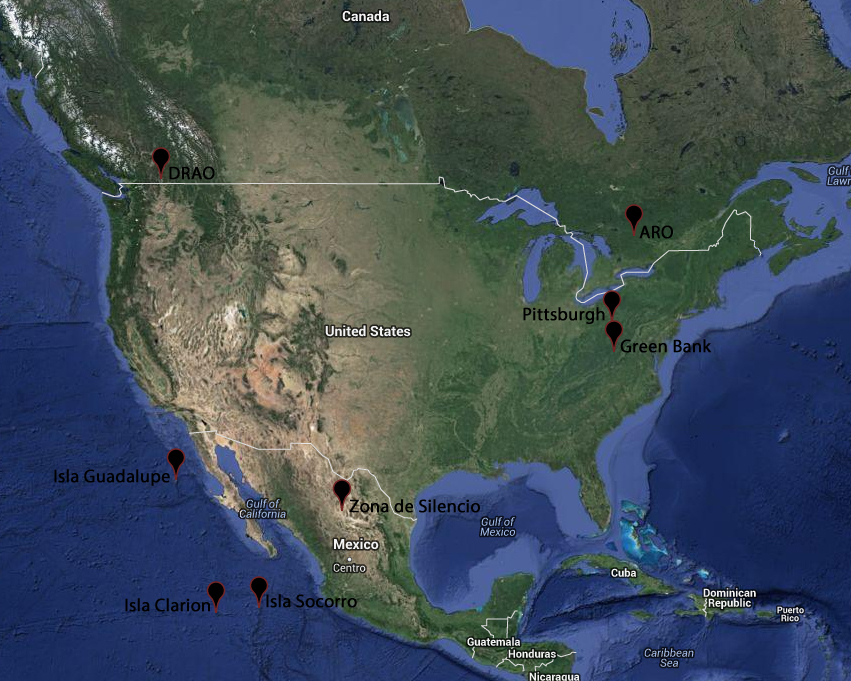
\includegraphics[width=0.95\textwidth]{RFI_testing/figures/large_scale_site_map.jpg}
\caption{Map of evaluated sites in North America, created using Google Maps.}
\label{Fig:site_map}
\end{center}
\end{figure}

The results of this measurement are shown in Figure \ref{Fig:resflux}. The measured signal was slightly higher than expected signal. Some of this difference was tied to the effective Spectrum Analyzer bandwidth ($30 kHz$), which is larger than the $10 kHz$ bandwidth quoted in the analyzer specifications from the manufacturer. The remainder of the difference may come from additional noise in the system or uncertainty in the noise figure meter values, but it is roughly flat in frequency. 

Because we use the same kit at all the sites, any systematic noise contribution such as the uncertainty in the $50 \Omega$ data found in Figure \ref{Fig:resflux} is constant across all datasets. 

\begin{figure}[tb]
\begin{center}
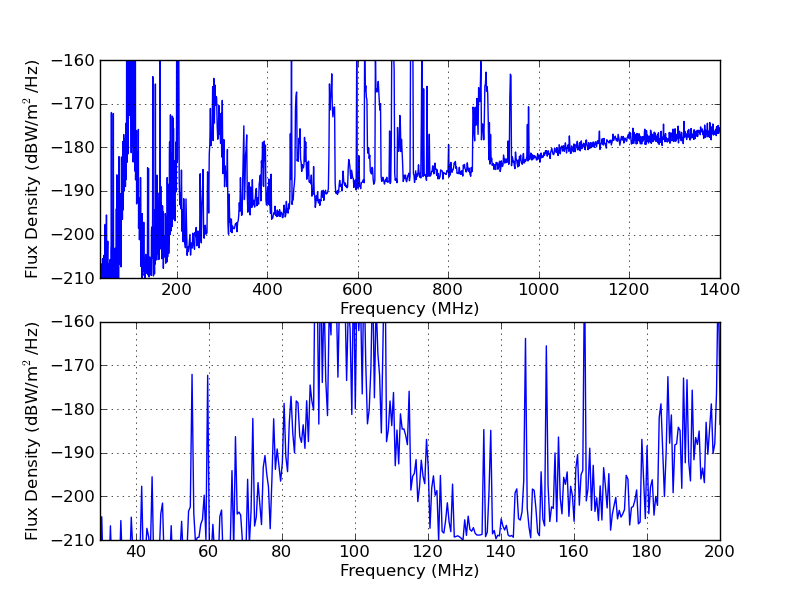
\includegraphics[width=0.9\linewidth]{RFI_testing/figures/Pittsburgh_cal.png}
\caption{RFI measurement at Carnegie Mellon University in Pittsburgh, Pennsylvania collected April 23rd, 2009. In the data, there are many RFI sources that produce signals that have a magnitude above the plotted range. These strong RFI signals produce inter-modulations that corrupt data outside of the actual frequencies of the RFI. For example, strong FM signals cause inter-modulation below  $88 MHz$ and above $108 MHz$. }
\label{Fig:pghcal}
\end{center}
\end{figure}



\section{Existing Site Evaluations}

Using the site testing kit discussed in Section \ref{Sec:site_kit}, data was taken at each of the sites shown in Figure \ref{Fig:site_map}. The portability of the kit (it packs up into the small suitcase and poster tube shown in Figure \ref{Fig:site_kit}) allows it to be easily transported to each of the sites. 


\subsection{Carnegie Mellon University Pittsburgh, PA, USA}

Carnegie Mellon University is located in the city of Pittsburgh ($40^\circ 26'30''$ N, $80^\circ 00' 00''$ W), home to several universities and possessing a population of over 300,000. As should be expected, the radio environment in Pittsburgh is full of RFI with signals of such magnitude that they overload test equipment. Figure \ref{Fig:pghcal} shows the RFI environment in Pittsburgh as measured with the site testing kit. The RFI signals are so loud in Pittsburgh that they overload the Spectrum Analyzer. 

To try and lower the RFI levels to measurable levels, we removed one stage of amplification from the system for the low frequency data. This is why the noise floor in Figure \ref{Fig:pghcal} is lower at low frequencies than it is in the other datasets. Amplification removal was designed to minimize the inter-modulation which begins to occur when there are RFI signals larger than $-170 \frac{dB \;W}{m^2 Hz}$. However, even with the amplifier removed from the system some of the RFI signals were still above the inter-modulation cutoff. For example, strong FM signals cause inter-modulation below $88 MHz$ and above $108 MHz$ in the Pittsburgh data. 


\begin{figure}[htb]
\centering
\begin{minipage}[b]{0.47\textwidth}
\centering
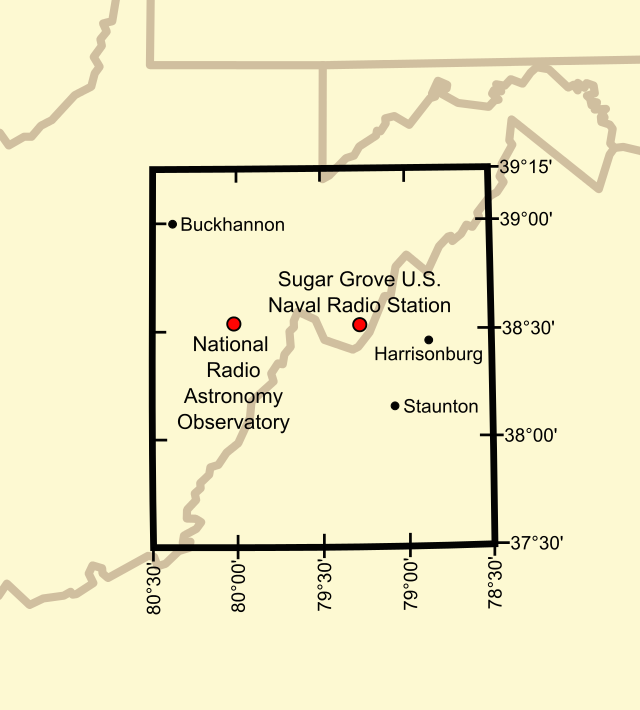
\includegraphics[width=0.75\linewidth]{RFI_testing/figures/National_Radio_Quiet_Zone.png}
\caption{Extent of the U.S. National Radio Quiet Zone around the Green Bank Site.}
\label{Fig:nrqz}
\end{minipage}%
\begin{minipage}[b]{0.02\textwidth}
\hspace{1cm}
\end{minipage}%
\begin{minipage}[b]{0.47\textwidth}
\centering
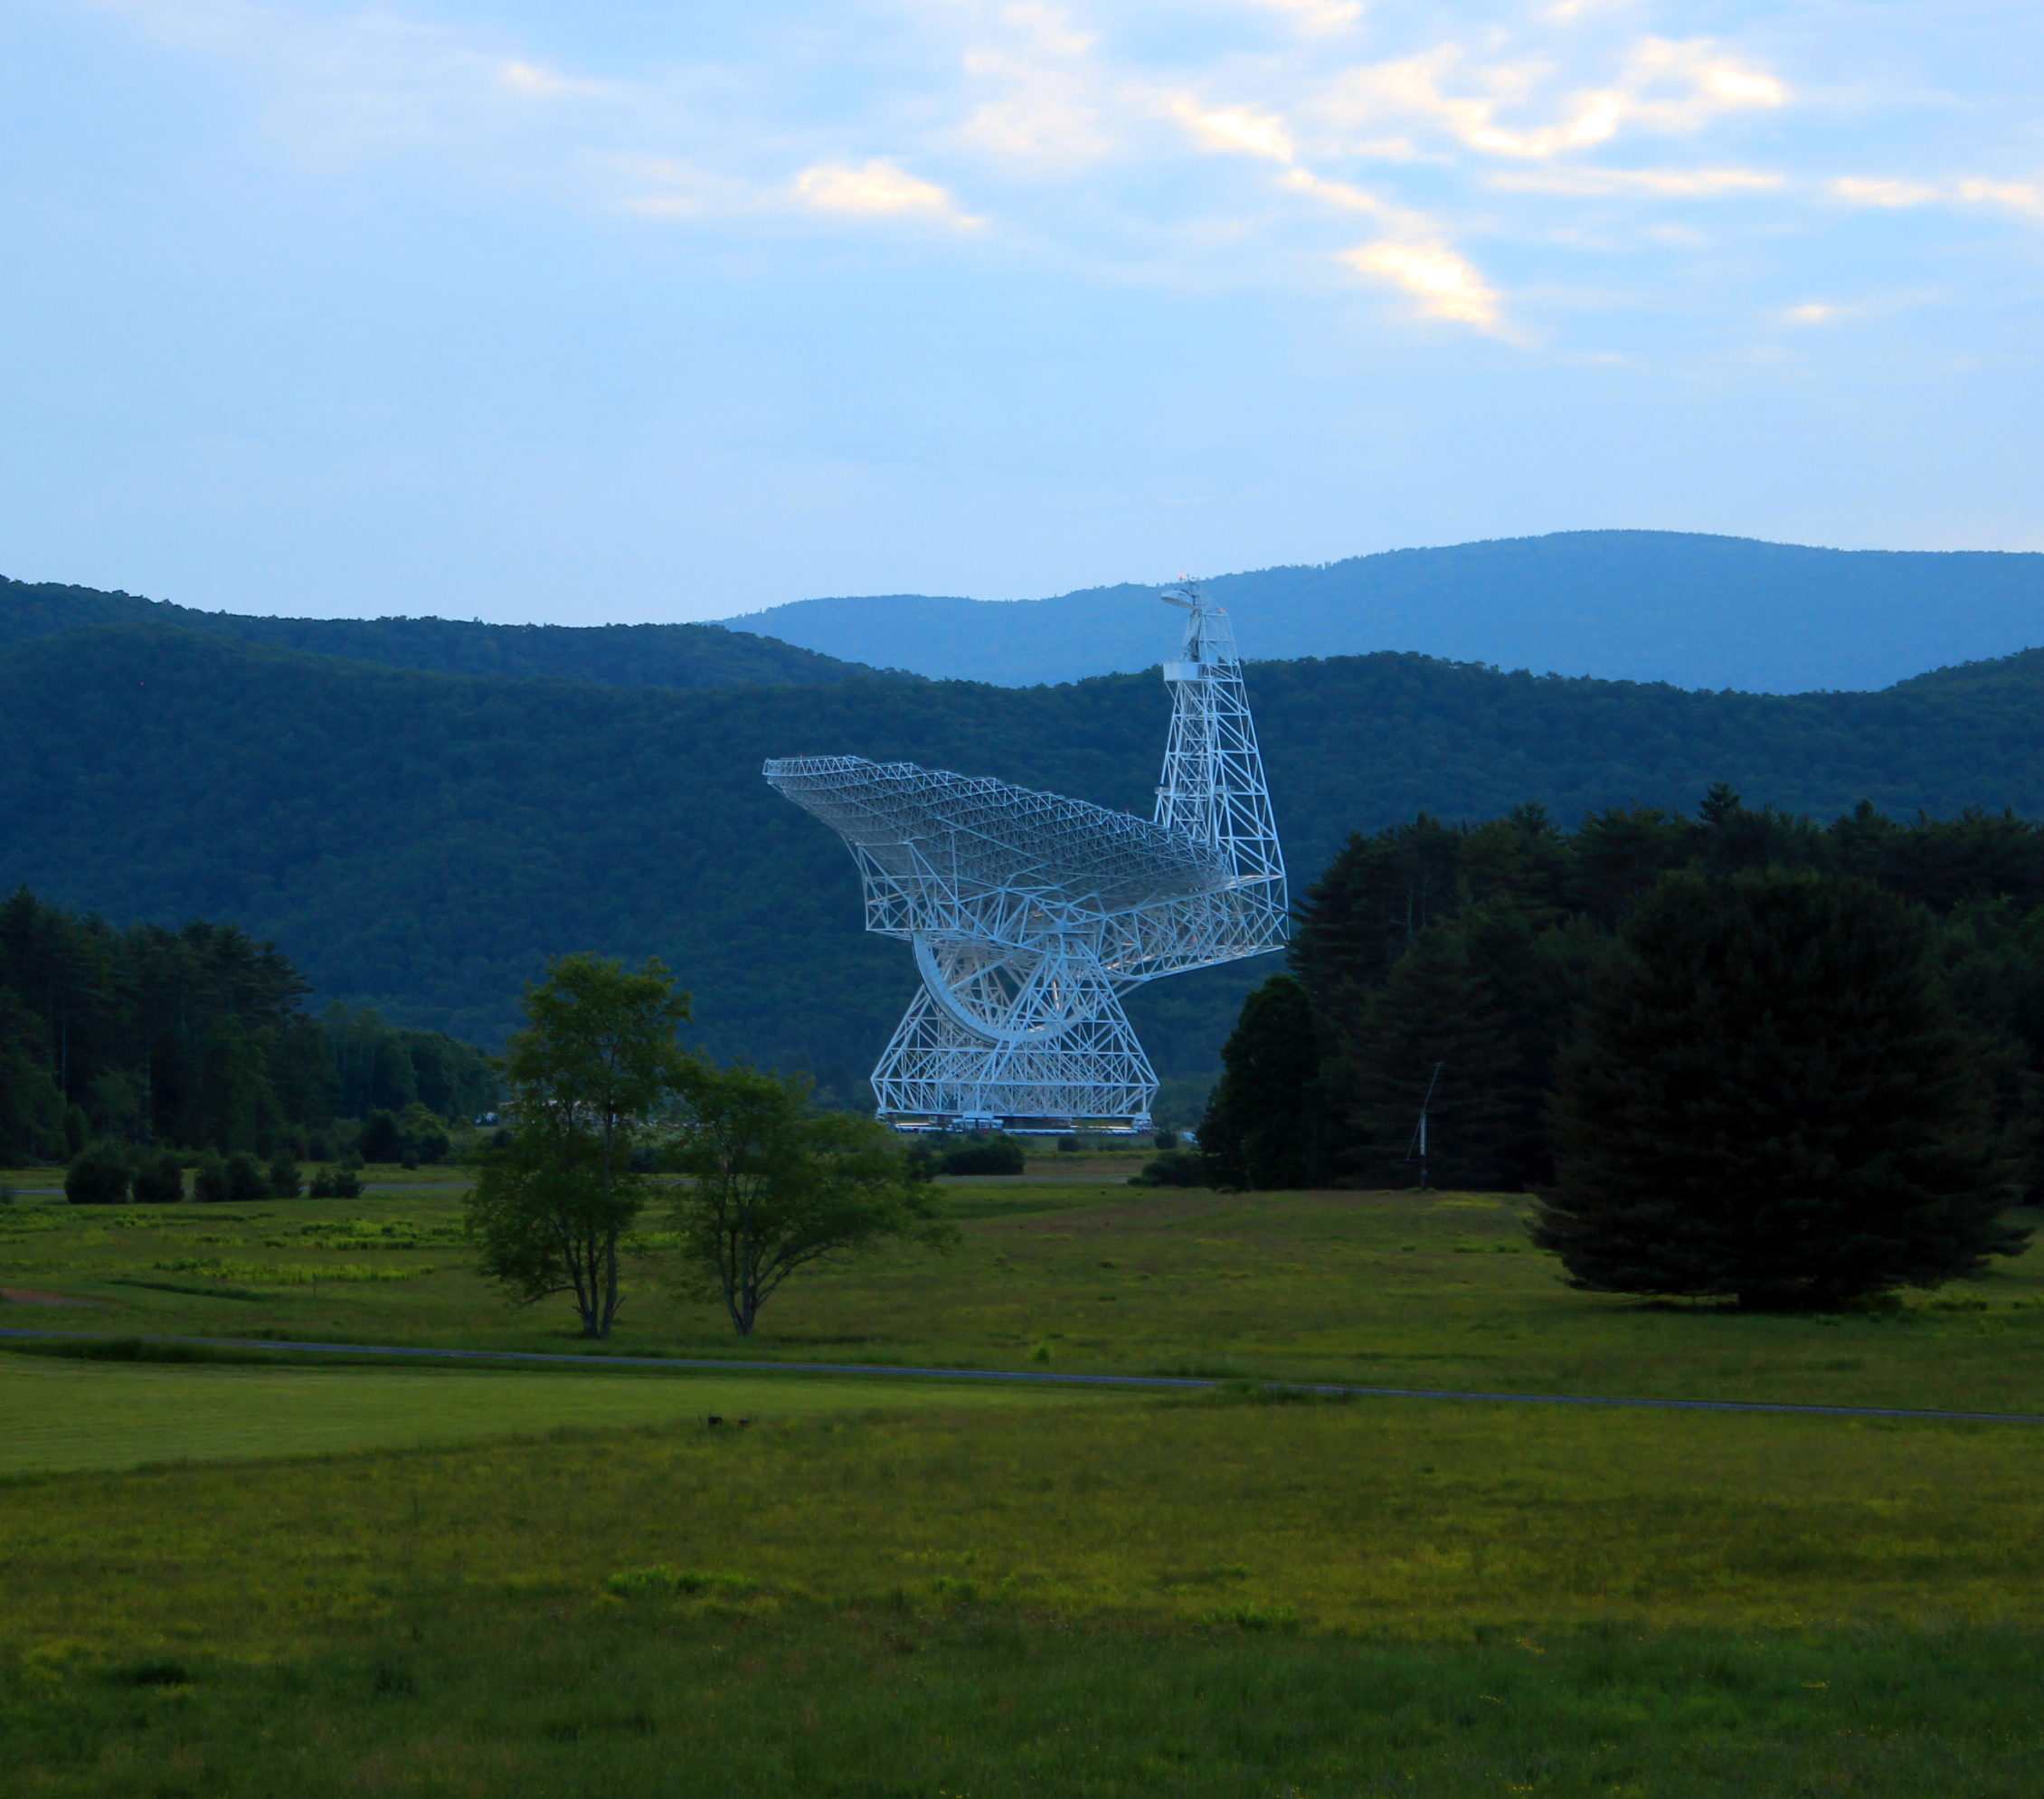
\includegraphics[width=0.95\linewidth]{RFI_testing/figures/gbt_site.jpg}
\caption{Robert C. Byrd Green Bank Radio Telescope as viewed from the site observation deck. }
\label{Fig:gbt}
\end{minipage}
\end{figure}

\begin{figure}[htb]
\begin{center}
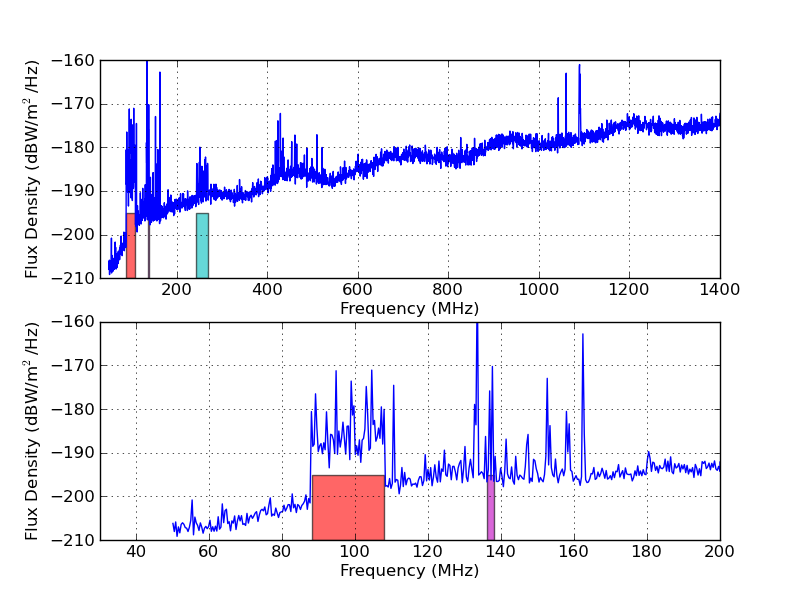
\includegraphics[width=0.9\linewidth]{RFI_testing/figures/GBT_bands.png}
\caption{RFI measurement at the NRAO Green Bank site collected on May 18th, 2010. In the plot, colored boxes indicate bands of well known RFI sources. Red is the FM band, Purple is the Orbcom satellite band, and Cyan is the military satellite band. Additional spikes in the data come from RFI sources not in the indicated bands. Large scale sinusoidal variation (or ringing) in the spectrum is caused by cable reflections in the system and is common to all data collected with the site testing kit. }
\label{Fig:gbtrfi}
\end{center}
\end{figure}


\subsection{National Radio Astronomy Observatory (NRAO) Green Bank}

The National Radio Astronomy Observatory (NRAO) is a research center funded by the U.S. National Science Foundation (NSF). It maintains several telesopes in radio quiet locations. One of these locations is in Green Bank, West Virginia inside the U.S. National Radio Quiet Zone in Virginia and West Virginia (see Figure \ref{Fig:nrqz}). Within this zone, radio broadcasts at all frequencies are minimized by law. This provides a relatively quiet RFI environment. 

The Green Bank site ($38^\circ 25' 59''$ N, $79^\circ 50' 23''$ W) hosts a number of radio telescopes including the $100 \; m$ Robert C. Byrd Green Bank Radio Telescope (see Figure \ref{Fig:gbt}). As an NRAO facility, the site has a full staff and facilities including housing, power, and other amenities. Located off a local highway, the site is a 4-5 hour drive from Pittsburgh. 

Looking at the data from the site testing kit, we find that the size of the radio quiet zone (about 34,000 $km^2$) is sufficient for higher frequencies but is too small at lower frequencies. As you can see in Figure \ref{Fig:gbtrfi}, there are specific bands of frequencies below $600 MHz$ where there is still a great deal of RFI. Some of these bands are indicated with colored boxes (red is the FM band, magenta is an orbcom satellite band and cyan is a military satellite band). 

Beyond the RFI, one of the other features of the site test data is a large scale sinusoidal variation (or ringing) in frequency. This variation is caused by reflections in the $50 \; cm$ cable between the antenna and first stage amplifier. One of the useful things about this ringing is that it provides a check that the system is working, because if one or more of the amplifiers has blown there is no ringing present in the data. Such a cross check is particularly useful in radio quiet areas, where there may not be much of a difference in the spectrum if the amplifier is malfunctioning. 

\begin{figure}[htb]
\begin{center}
\includegraphics[width=0.9\linewidth]{RFI_testing/figures/penticton_rect.jpg}
\caption{Some of the DRAO facilities and telescopes (CHIME pathfinder in foreground). }
\label{Fig:penticton}
\end{center}
\end{figure}

\begin{figure}[htb]
\begin{center}
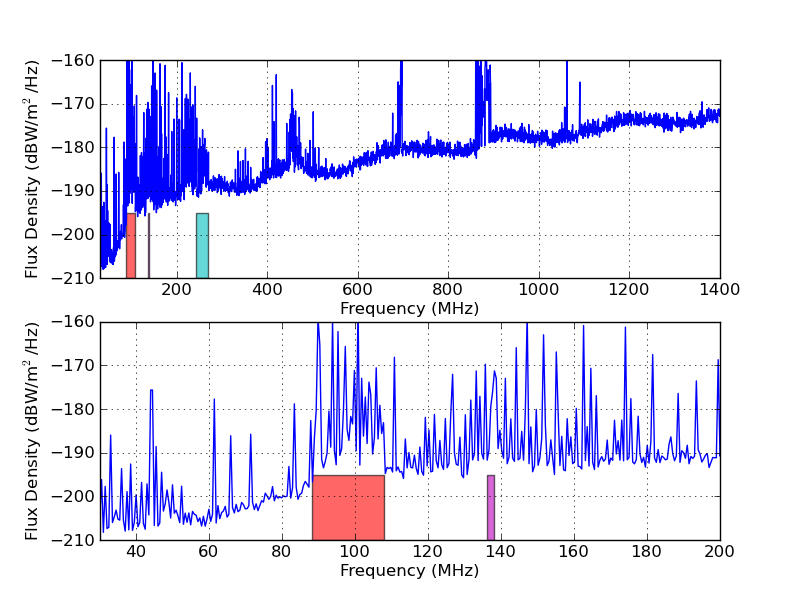
\includegraphics[width=0.9\linewidth]{RFI_testing/figures/DRAO_bands.png}
\caption{RFI measurement at the DRAO Penticton site collected on December 14th, 2009. DRAO has excessive RFI in the entire spectrum below $400 MHz$ and is generally noisier than Green Bank. Because some of these signals (particularly the FM band) are above the inter-modulation cutoff, some of the smaller spikes in known clear bands are believed to be caused by inter-modulation. In the plot, colored boxes again indicate bands of well known RFI sources (Red= FM band, Purple = Orbcom satellite band, and Cyan = military satellite band).   }
\label{Fig:draorfi}
\end{center}
\end{figure}

\begin{figure}[tb]
\begin{center}
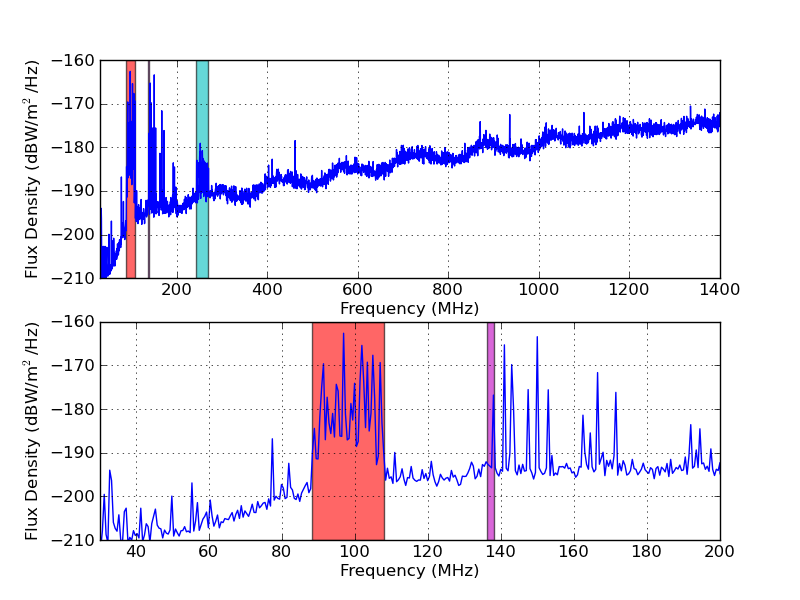
\includegraphics[width=0.9\linewidth]{RFI_testing/figures/ALG_bands.png}
\caption{RFI measurement at the ARO Algonquin site collected on September 12th, 2012. Like the GBT site, the ARO site is quiet at high frequencies compared to DRAO or Pittsburgh. However, significant RFI is still present below $300 MHz$. In the plot, colored boxes again indicate bands of well known RFI sources (Red= FM band, Purple = Orbcom satellite band, and Cyan = military satellite band).}
\label{Fig:arorfi}
%\end{minipage}
\end{center}
\end{figure}


\subsection{Dominion Radio Astrophysical Observatory (DRAO)}

The Dominion Radio Astrophysical Observatory (DRAO) is a Canadian radio astronomy site ($49^\circ 19' 15.6''$ N, $119^\circ 37' 26.4''$ W). Located near Penticton, British Columbia in the south-central part of the province, DRAO has a number of radio telescopes on site and the Canadian Hydrogen Intensity Mapping Experiment (CHIME) system is currently being built there. Figure \ref{Fig:penticton} shows some of the facilities at DRAO including part of the CHIME pathfinder in the foreground. 

The site can be easily accessed by car, with on-site facilities available for researchers. It is also a $\sim$30 minute drive from Penticton, a town with a population of over 30,000. 

Like the NRAO Green Bank site, the DRAO site has insufficient isolation from civilization to provide a radio quiet environment at the lower frequencies. There is significant RFI contamination for most frequencies below $500 MHz$ at this site (see Figure \ref{Fig:draorfi}). Given DRAO's location close to Penticton, some of the signals in the FM band are loud enough to cause intermodulation of signals into some of the frequencies that are actually clean. This can be seen in the band between $108-136 MHz$, the dedicated aerospace band, which should be clear of RFI everywhere in the world. 


\subsection{Algonquin Radio Observatory (ARO)}

The Algonquin Radio Observatory (ARO) is a single instrument Canadian radio astronomy site ($45^\circ 57' 19.8''$ N, $78^\circ 4' 23''$ W). Located in the center of Algonquin Provincial Park in Ontario, Canada; the site is only accessible by logging roads, which are gravel but can be driven by most vehicles during the summer. ARO is also accessible in an emergency via helicopter, but this mode of transportation is not commonly used. ARO does have power and full amenities on site including housing for researchers. 

Although the site has excellent radio quiet properties at higher frequencies, it is still relatively close (about $200-250 \; km$) to the major Canadian metropolitan areas of Toronto and Ottawa. When we set up our site test at ARO, we found that although the rest of the spectrum is quite clean there is still significant RFI below $300 MHz$ (see Figure \ref{Fig:arorfi}), including in the FM radio band. 


\begin{figure}[htb]
\begin{center}
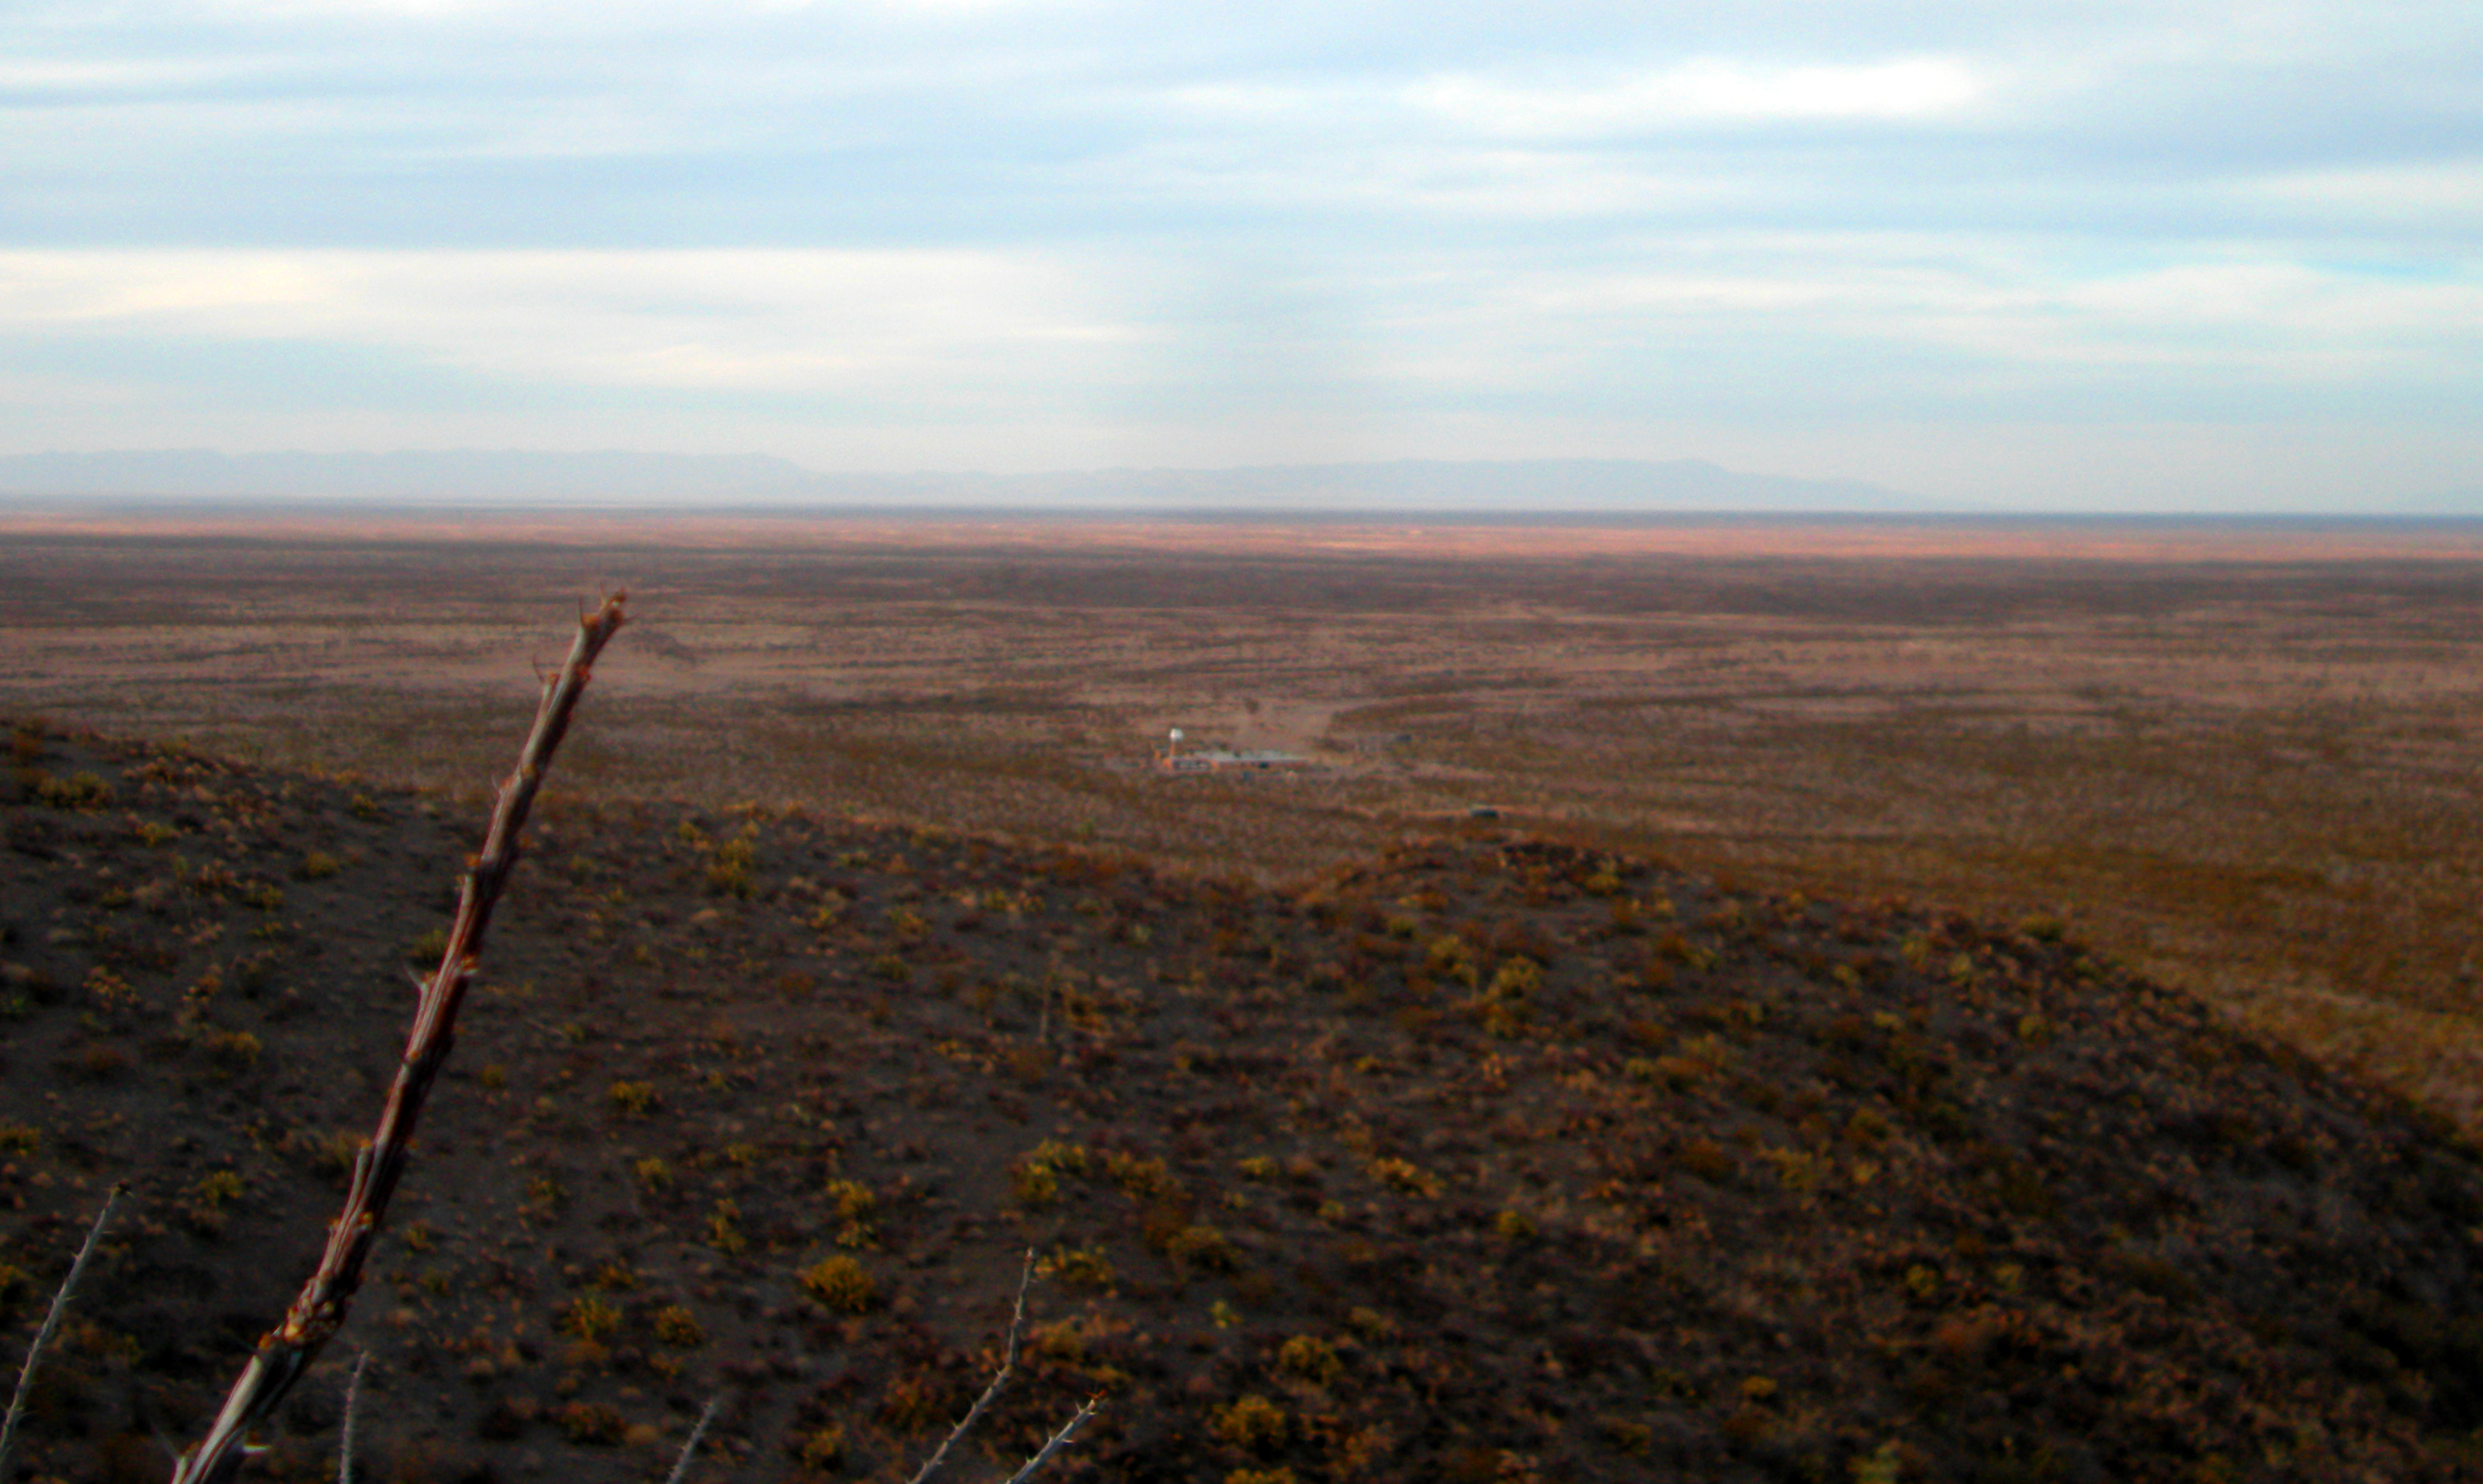
\includegraphics[width=0.9\linewidth]{RFI_testing/figures/zds_overview_shot.jpg}
\caption{View of the Zona del Silencio from one of the nearby peaks. The ecologist's camp where we stayed while running our tests is in the center of the picture.}
\label{Fig:zdsover}
\end{center}
\end{figure}

\begin{figure}[htb]
\begin{center}
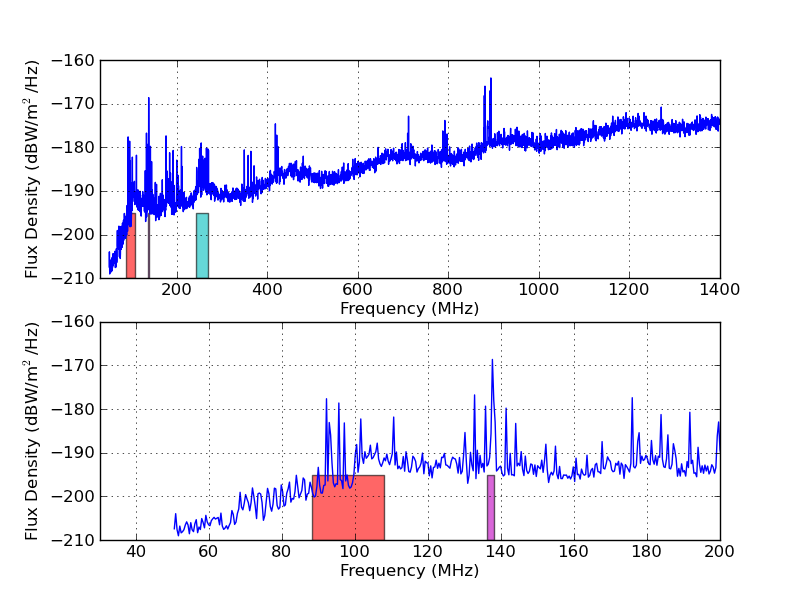
\includegraphics[width=0.9\linewidth]{RFI_testing/figures/ZdS_halfway_in_bands.png}
\caption{RFI measurement near the ecologist's camp in the Zona del Silencio, collected on May 5th, 2010. The Zona del Silencio site has even less RFI than the previous sites at low freuqencies, although some RFI spikes are still present. In the plot, colored boxes again indicate bands of well known RFI sources (Red= FM band, Purple = Orbcom satellite band, and Cyan = military satellite band).}
\label{Fig:zdsendrfi}
\end{center}
\end{figure}



\section{New Site Evaluations}

Evaluation of these existing radio quiet sites demonstrated a clear need for sites whose RFI environments are cleaner at frequencies below $500 MHz$. However, locating such sites can be difficult as the distances required begin to grow large. Here, I report on a couple of potential sites in Mexico that have significant improvement in their low frequency RFI strength compared to the existing sites. 


\subsection{La Zona del Silencio}

$''$Zona del Silencio$''$ ($26^\circ 41' 10.3''$ N, $103^\circ 44' 50.9''$ W) is a radio quiet region in the Mapimi part of the Chihuahuan desert in Northern Mexico. It has a reputation as a mysterious radio quiet zone due to historic events similar to the Bermuda Triangle, but in a desert setting. Some of its radio quiet status may be due to the local geography as the desert is a flat plateau, but there are mountains between it and any significant civilization. The closest major metropolitan area is Torre\'{o}n, over $150 km$ south of the zone center. The zone is also a protected biosphere reserve maintained by Mexcio's $''$Comisi\'{o}n Nacional de \'{A}reas Naturales Protegidas$''$ (CONANP). 

\subsubsection{Logistics and Current Infrastructure}

While major highways can be found along the outside of the region, the only roads in and out of the site are poorly maintained dirt roads that require 4-wheel drive.

Permanent settlements are not allowed within the biosphere reserve. However, at the center of the site is a camp for ecologists studying the biosphere found in the reserve. The site has minimal housing with solar cells charging batteries for power but all water on site has to be brought in from outside. 

For our site test, we got special permission to stay at the ecologist's camp called $''$Laboratorio del Desierto$''$, shown in Figure \ref{Fig:zdsover}.

\subsubsection{Environmental Impacts}

During the site testing, we were able to observe the general climate of the site as a consideration for future deployments. One of the challenges we observed was the prevalence of dust due to the arid climate. All our equipment had to be well protected from dust, especially during transport to and from the site. If not properly shielded, dust can cause electronic equipment to malfunction. 

Another potential challenge is the temperature variation associated with the climate. Even within a single day we saw a strong difference between night and day temperatures. Temperature variation can create variance in collected data from a telescope, making the desired signals more difficult to detect. 

\subsubsection{Measurements}

On this first site test, we chose to measure the site quality at a specific location near the center of the zone where RFI was expected to be at a miniumum. Setting up near the ecology camp but far enough away to prevent contamination by the local electronics, we measured extremely low RFI levels as is shown in Figure \ref{Fig:zdsendrfi}.

There is still some noise at lower frequencies, but the FM band is considerably quieter than at any of the existing radio quiet sites that we had tested. 

Further testing at this site should include a survey of a wide range of locations within the $''$Zona del Silencio$''$ to map out the region's radio quiet properties. 

\begin{figure}[htb]
\centering
\begin{minipage}[b]{0.47\textwidth}
\centering
\includegraphics[width=0.95\linewidth]{RFI_testing/figures/isla_guadalupe_site_map.jpg}
\caption{Map of Isla Guadalupe with the sites of interest indicated.}
\label{Fig:guadmap}
\end{minipage}%
\begin{minipage}[b]{0.02\textwidth}
\hspace{1cm}
\end{minipage}%
\begin{minipage}[b]{0.47\textwidth}
\centering
\includegraphics[width=0.95\linewidth]{RFI_testing/figures/omar_site_test_guad.jpg}
\caption{Collecting data with the site testing equipment on Isla Guadalupe.}
\label{Fig:guadsite}
\end{minipage}
\end{figure}


\begin{figure}[tb]
\centering
\begin{minipage}[b]{0.455\textwidth}
\centering
\includegraphics[width=0.95\linewidth]{RFI_testing/figures/guad_plane.jpg}
\caption{Airplane used for access to Isla Guadalupe.}
\label{Fig:guadplane}
\end{minipage}%
\begin{minipage}[b]{0.02\textwidth}
\hspace{1cm}
\end{minipage}%
\begin{minipage}[b]{0.485\textwidth}
\centering
\includegraphics[width=0.95\linewidth]{RFI_testing/figures/guad_plateau_plane.jpg}
\caption{View of the plateau with the fishing village from the airplane.}
\label{Fig:guadplateau}
\end{minipage}
\end{figure}


\subsection{Isla Guadalupe}

Isla Guadalupe ($29^\circ 1' 51''$ N, $118^\circ 16' 48''$ W) is a small volcanic island located about 250 $km$ west of Baja California in Mexico. The island has an area of $\sim$250 $km^2$, with two significant peaks along the north-south axis of the island. A biosphere reserve, access to Guadalupe is limited to a few groups. Namely, the Mexican government and Navy ($''$Secretar\'{i}a de Gobernaci\'{o}n$''$ and $''$Secretar\'{i}a de Marina$''$), ecologists studying the land and marine life such as the $''$Grupo de Ecolog\'{i}a y Conservaci\'{o}n de Islas A.C.$''$ (GECI) and CONANP, and the local fishing cooperative ($''$Sociedad Cooperativa d Producci\'{o}n Pesquera de Participaci\'{o}n Estatal Abuloneros y Langosteros, S.C.L.$''$). We were able to travel to Isla Guadalupe with support from these organizations. 

\begin{figure}[htb]
\centering
\begin{minipage}[b]{0.43\textwidth}
\centering
\includegraphics[width=0.95\linewidth]{RFI_testing/figures/mex_navy_arrival.jpg}
\caption{Mexican naval vessel as it arrived at Isla Guadalupe to deliver supplies and pick us up.}
\label{Fig:guadboat}
\end{minipage}%
\begin{minipage}[b]{0.02\textwidth}
\hspace{1cm}
\end{minipage}%
\begin{minipage}[b]{0.51\textwidth}
\centering
\includegraphics[width=0.95\linewidth]{RFI_testing/figures/mex_navy_onboard.jpg}
\caption{View from onboard the Mexican naval vessel during the trip back to the Port of Ensenada.}
\label{Fig:guadonboard}
\end{minipage}
\end{figure}

\subsubsection{Logistics and Current Infrastructure}

Access to Isla Guadalupe requires one of two transport methods. First, small planes such as the one shown in Figure \ref{Fig:guadplane} can fly from the city of Ensenada in Baja California to the island, where there is a small landing strip. This flight takes 1-2 hours and can only be made during good weather. On several of our visits to Isla Guadalupe, this was our method of transport. However, each flight costs about \$2000 and can only carry $\sim$600 $kg$ including both people and supplies. 

A much cheaper alternative is transport with the supply ship that the Mexican Navy uses to support its base on Guadalupe. This supply ship, shown in Figures \ref{Fig:guadboat} and \ref{Fig:guadonboard}, deploys once a month from the port of Ensenada; stopping first at Isla Guadalupe, then Isla Cedros, then returning to Ensenada with a total travel time of about three days. Travel via this route requires passengers to $''$camp out$''$ by sleeping on the deck of the ship during transit. In addition, since passengers are hitching a ride with the ship they have no control over changes in ship deployment (eg delays or re-routing) that may change the departure or arrival schedule. This places strictures on any deployments to Isla Guadalupe that must be accounted for in planning the trip. In comparison to the flight costs, passage on the supply ship is only \$50 per person (for food) with minimal weight limits as some of the other passengers have been known to even transport cars via the supply ship. 

While on Guadalupe we had the option of staying with the ecologists, the fishing village or the navy base. Each provided some level of logistical support, but all had limited resources. 

The ecology camp is a small camp with about 5-15 researchers in residence at any given time. Housing, including running water, is available at the site for the researchers and their visitors but there is little to no plumbing, so the bathroom is a dry toilet.  Since power is supplied by solar panels and batteries, it is pretty limited, especially at night. However, during the day there is regular internet access via satellite. Since it is a small camp, food is served communally, with everyone taking turns for cooking and cleaning responsibilities. 

In contrast, the fishing village has a semi-permanent population of about 100 people and can be seen in Figure \ref{Fig:guadplateau}. The fishing village is a cooperative, which means that resources and profits are shared within the community. Houses are assigned to individual families who are currently living on site, as opposed to their main homes on the mainland. Furnishings in the houses are haphazard since all of the furnishings had to be brought in on boats. There is a sewage plant for the village, but no running water (so flushing the toilet means dumping sea water into the bowl). Instead, water is supplied by a desalination plant and each family has barrels of both clean water and sea water at their homes. 

Power in the village is supplied by a large generator that runs throughout the day, except for a few hour siesta in the mid-afternoon and in the middle of the night. Food supplies are purchased by the cooperative and shipped in via the supply boat. Bulk supplies are stored at the community store where each family can $''$purchase$''$ food by signing out the items they need and debiting the cost to their share of the cooperative's profits. When we stayed in the fishing village, we were given use of one of the houses that was currently unoccupied. Meanwhile, we paid one of the fishermen's wives to cook for us.  

Like the ecology camp, the military (naval) base is extremely minimal in scope. There is only a small contingent of personnel ($\sim$10) at any time, so there are only a few buildings with a small generator and everyone takes turns cooking, etc. Water is also limited at the base, since the only natural water source on the island is located at the peak near the ecology camp. 

\begin{figure}[tb]
\begin{center}
\includegraphics[width=0.9\linewidth]{RFI_testing/figures/GI_3__bands.png}
\caption{RFI measurement from the ecology camp at the summit of Isla Guadalupe collected on November 1st, 2012. At this site, the elevation means that the line of sight is longer and RFI can be seen from further distances than at lower elevations. Despite this fact, the spectrum is mostly free from RFI above $300 MHz$. In the plot, colored boxes again indicate bands of well known RFI sources (Red= FM band, Purple = Orbcom satellite band, and Cyan = military satellite band).}
\label{Fig:guadsummit}
\end{center}
\end{figure}

\subsubsection{Environmental Impacts}

Located in the Pacific Ocean, in the midst of the California current, Isla Guadalupe is quite temperate for its latitude. The high elevation of its peaks (nearly $1300 \; m$) means that there are two distinct microclimates (one near sea level and one at high elevations). One reason for this contrast is that the island's peaks sit above the low cloud layer, making the higher altitudes warmer and generally clearer. Additional impacts include flash flooding in the lower areas of the island during the wet season and wind and dust interfering with system at any time. 

Guadalupe's location puts it north of the main Pacific hurricane impact zone, but during the hurricane season storms pass over the island. In addition, the naval supply vessel often has its schedule changed during this season due rough seas from the storms. As an example, we had to change our deployment strategy from boat transit to plane in October 2012 due to Hurricane Paul, which hit the island as a weak tropical depression. This means that the optimal time to visit Isla Guadalupe is during the hurricane off-season (November to June). 


\begin{figure}[htb]
\begin{center}
\includegraphics[width=0.9\linewidth]{RFI_testing/figures/GI_2__bands.png}
\caption{RFI measurement from the lava flow near the fishing village at Isla Guadalupe collected on November 1st, 2012. At this site, the lower elevation and the mountain between the lava flow and the mainland act as an RFI shield. This means that even the lowest frequency bands are relatively clear of RFI. In the plot, colored boxes again indicate bands of well known RFI sources (Red= FM band, Purple = Orbcom satellite band, and Cyan = military satellite band).}
\label{Fig:guadlow}
\end{center}
\end{figure}

\subsubsection{Measurements}

Upon arrival on Guadalupe, several sites were studied for potential deployment. Site 1 was near the ecology camp at the summit of the northern peak of the island, site 2 was near the fishing village on the western side of the island and site 3 was near the military base on the southern tip of the island. The exact positions of these sites are shown in Figure \ref{Fig:guadmap}. I am only showing results from sites 1 and 2 as they have the most dramatic differences in RFI quality. 

Figure \ref{Fig:guadsummit} shows the RFI signals from site 1 at the northern summit. Just as at existing radio quiet sites the spectrum is quite clean at high frequencies. However, as we move to low frequencies there is still some significant RFI, particularly in the FM radio band. Much of this noise is coming from the radio stations in San Diego and Ensenada, including some channels which can actually be heard with a hand-held radio. In this case, the elevation is actually a detriment as the height extends the line of sight for the RFI testing antenna. 

In contrast, Figure \ref{Fig:guadlow} shows the RFI signals from site 2 near the fishing village. Here the combination of low elevation, distance from the mainland and the peaks of Guadalupe act as an excellent shield to minimize the RFI in the FM band to nearly undetectable levels. As seen from the plane in Figure \ref{Fig:guadplateau}, this plateau has significant elevations to the north, south, and east, effectively shielding it from mainland Mexico and Baja California. 

\begin{figure}[htb]
\begin{center}
\includegraphics[width=0.8\linewidth]{RFI_testing/figures/site_testing_south.jpg}
\caption{Potential future site testing locations in the Southern Hemisphere. Image made using Google Maps.}
\label{Fig:site_map_south}
\end{center}
\end{figure}



\section{Future Sites}

Deployment in June 2013 to Isla Guadalupe with the SCI-HI experiment demonstrated that while the island has very low RFI in general, there is still some residual RFI in the FM band ($88 MHz \leq f \leq 108 MHz$). This RFI makes the band un-usable for the SCI-HI experiment. In order to continue the SCI-HI experiment, several potential sites have been identified.

\begin{enumerate}

\item Isla Socorro and Isla Clari\'{o}n, off the west coast of Mexico, (see Figure \ref{Fig:site_map}) are under investigation as further remote sites in the northern hemisphere.

\item Marion Island, off the coast of South Africa, (see Figure \ref{Fig:site_map_south}) has been identified as an excellent potential site in the southern hemisphere.

\item Additional sites in the southern hemisphere, such as the Antarctic bases and Gough Island, have longer term potential as future sites for testing. 

\end{enumerate}

\subsection{New Sites in Mexico}

Like Isla Guadalupe, Socorro and Clari\'{o}n are small volcanic islands in the Pacific Ocean off the coast of Mexico. Isla Socorro ($18^\circ 47' 4''$ N, $110^\circ 58' 30''$ W) has an area of $\sim$130 $km^2$ and is about 600 $km$ off the western coast of Mexico. Isla Clari\'{o}n ($18^\circ 22'$ N, $114^\circ 44'$ W) has an area of $\sim$20 $km^2$ and is over 700 $km$ from the mainland.

Possessions of Mexico, both islands are ecological reserves with no permanent population. Both islands also have naval installations, although the base on Socorro is significantly larger than the one on Clari\'{o}n. Access to these islands requires permits from the Mexican government, and can be achieved through passage with the Mexican Navy. The Socorro and Clari\'{o}n bases are supported by twice monthly supply boats, and passage can be arranged with the Navy using these boats. 

Weather plays a significant role in limiting visits to Socorro and Clari\'{o}n because most of the Pacific hurricanes impact the islands each year. Therefore, access for research is limited to the off-season (December to May). Site testing on Socorro and Clari\'{o}n is planned for the future.


\subsection{New Sites in South Africa and Antarctica} \label{Sec:SA_site}

Meanwhile, Marion Island ($46^\circ 52' 34''$ S, $37^\circ 51' 32''$ E) is a small volcanic island in the sub-Antarctic Indian Ocean owned by South Africa (see Figure \ref{Fig:site_map_south}). It has an area of $\sim$ 225 $km^2$, with a single peak $\sim$1 $km$ in height. Located $>$2000 $km$ from the South African coast, this island is expected to have excellent isolation from RFI in the FM band. 

Access to the island is provided by the South African National Antarctic Programme (SANAP), which oversees research done on Marion and other islands. Most of the research on the island is focused on the native species and climate. Travel to the island happens once a year, with most of the research occurring over the $\sim$1 month deployment. A small crew remains on the island over the rest of the year ($\sim$11 months). 

Professor Jonathan Sievers at the University of Kwa-Zulu Natal in South Africa was recently awarded a grant through SANAP to investigate and use Marion Island as a site for radio astronomy. As a part of this grant, I will be travelling to Marion Island on the 2015 SANAP trip, which takes place from April to May 2015. During this trip, I will make measurements around the island. These measurements will be used to evaluate the overall RFI environment and identify the best location to place an experiment. I will also deploy the SCI-HI experiment at the location I identify during my evaluation. 



\chapter{Low Frequency Radio Astronomy and the Earth's Ionosphere}\label{Ch:Iono}

\section{Overview}
Beyond the effects of RFI, the Earth's atmosphere has additional impacts on low frequency radio signals from the universe. These impacts come from interactions between the incoming radio signals and the free electrons in the ionosphere. Impacts include refraction and absorption of radio frequency photons. 

These impacts are dependent on the time and geographic location variant structure of the ionosphere. However, in general ionospheric impacts have the potential to mask the \cm signal, as they introduce additional frequency dependent structure into the measured signal. Therefore, it is necessary to quantify and address ionospheric impacts in any \cm measurement. 


\begin{figure}[htb]
\centering
\begin{minipage}[b]{0.48\textwidth}
\centering
\begin{tabular}{|c|c|}
\hline
Layer & Altitude Range (km) \\
\hline
D & 60-100 \\
\hline
E & 100-150 \\
\hline
F1 & 150-250 \\
\hline
F2 & 250-1000+ \\
\hline
\end{tabular}
\caption{Average distribution of the Earth's ionosphere layers.}
\label{Tab:iono_layer}
\vspace{2cm}
\end{minipage}%
\begin{minipage}[b]{0.02\textwidth}
\hspace{1cm}
\end{minipage}%
\begin{minipage}[b]{0.48\textwidth}
\centering
\includegraphics[width=0.95\linewidth]{Ionosphere/figures/atmosphere_layers.jpg}
\caption{Idealized free electron density distribution in Earth's atmosphere showing the ionosphere's layers during day and night. }
\label{Fig:iono_layer}
\end{minipage}
\end{figure}

\section{Earth's Ionosphere}
To understand ionospheric impacts on the \cm signal we need to understand the ionosphere. Earth's ionosphere is located $60 - 1000+$ $km$ above the surface of the Earth and is made up of free electrons and ionized atoms. Neutral atoms in Earth's atmosphere are photoionized by solar radiation, which leads to an altitude dependent distribution of free electrons and ions in the atmosphere.

\subsection{Ionospheric Layers}
This distribution allows us to divide the ionosphere into altitude-dependent regions. The center of each region is defined by a local maximum in the free electrion density distribution as a function of altitude. The regions of the ionosphere are identified in Figure \ref{Tab:iono_layer}. The absolute maximum free electron density ($n_e$) is reached in the F2 layer and is $n_e \cong 10^5 cm^{-3}$ \cite{ionospheres}. 

The presence and width of the ionospheric layers is time dependent and fluctuates over the course of a day. During the day all the layers are present, but during the night some of the layers merge as shown in Figure \ref{Fig:iono_layer}. Electron density distribution also depends on the level of sunspot activity and the specific position (particularly the latitude) on the Earth \cite{thompson_2001}. 

\subsection{Ionosphere Properties}

\subsubsection{Plasma Frequency}
Free electrons in the ionosphere can be treated like a plasma and will modify the propogation of light. We can quantify it by defining a plasma frequency ($\nu_p$), which has a value equal to:

\begin{equation}
\nu_p = \frac{e}{2 \pi} \sqrt{\frac{n_e}{\varepsilon_0 m}} \cong 9 \sqrt{n_e} Hz
\end{equation}

where $n_e$ is in $m^{-3}$ \cite{thompson_2001}. This plasma frequency changes the index of refraction for the ionosphere compared to free space $n = \sqrt{1-\nu_p^2/\nu^2}$, where $\nu$ is the frequency of the light that is passing through the atmosphere \cite{thompson_2001}. 

\subsubsection{Cyclotron Frequency}
In addition to the plasma frequency due to free electrons, a static magnetic field in the ionsphere will lead to motion of the free electrons. This motion can be quantified using a gyrofrequency defined as ($\nu_B = eB/2 \pi m$), and has a typical magnitude of $\nu_B \cong 1.4 MHz$ \cite{thompson_2001}. 

In adding in the cyclotron frequency to the index of refraction, the direction of the magnetic field with respect to the incoming signal matters. This means that the impact of a static magnetic field will be polarized. This is the source of Faraday roation in Earth's atmosphere \cite{thompson_2001}. However, since the impact is proportional to $\nu_B/\nu$ and $\nu \gg \nu_B$ for our frequency band; we will neglect the impact from the Earth's magnetic field in the rest of the discussion. 


\begin{figure}[htb]
\begin{center}
\includegraphics[width=0.95\linewidth]{Ionosphere/figures/gps_sitemap.png}
\caption{Global Map of GPS Network stations used for the quasi-real time maps of $TEC$ available online at (iono.jpl.nasa.gov)}
\label{Fig:gps_stat}
\end{center}
\end{figure}

\begin{figure}[htb]
\centering
\begin{minipage}[b]{0.48\textwidth}
\centering
\includegraphics[width=0.95\linewidth]{Ionosphere/figures/TEC_map_20141013_18-40UT.png}
\caption{$TEC$ map for October 13th, 2014 at 18:40 UTC. (iono.jpl.nasa.gov)  }
\label{Fig:fall_tec_global}
\end{minipage}%
\begin{minipage}[b]{0.02\textwidth}
\hspace{1cm}
\end{minipage}%
\begin{minipage}[b]{0.48\textwidth}
\centering
\includegraphics[width=0.95\linewidth]{Ionosphere/figures/TEC_map_20150213_01-10UT.png}
\caption{$TEC$ map for February 13th, 2015 at 01:10 UTC. (iono.jpl.nasa.gov)  }
\label{Fig:winter_tec_global}
\end{minipage}
\end{figure}

\section{Total Electron Content}
Measurement of the number of free electrons at a given altitude ($n_e$) can be quite difficult. Instead, scientists typically measure the total electron content ($TEC$). $TEC$ is the integrated number of free electrons for a skewer through the atmosphere. It is defined as:

\begin{equation}
TEC = \int_0^\infty n_e (h) dh 
\end{equation}

where $h$ is the altitude \cite{thompson_2001}. $TEC$ is typically quoted in $TECU$, where $1 TECU$ corresponds to an average $n_e = 10^{16}$ electrons per $m^2$ \cite{vedantham_2014}. Total electron content is continually monitored on Earth using measurements from GPS stations around the world. This data is collected by a number of agencies that convert the data into maps. 

\subsection{Measuring $TEC$}
Real time maps of $TEC$ over the entire world are made by NASA JPL using the GPS stations shown in Figure \ref{Fig:gps_stat} and are available online\footnote{\url{http://iono.jpl.nasa.gov/latest_rti_global.html}}. The plots are based on a five minute average, and the image is updated online every five minutes. A couple of examples of these maps are Figures \ref{Fig:fall_tec_global} and \ref{Fig:winter_tec_global}, which show the measured $TEC$ distribution for two different times of day (and times of year). The bright region with high $TEC$ corresponds to the part of the globe currently receiving sunlight. Also, areas close to the equator are much brighter than areas near the poles in both the day and night regions.

\begin{figure}[htb]
\centering
\begin{minipage}[b]{0.48\textwidth}
\centering
\includegraphics[width=0.95\linewidth]{Ionosphere/figures/NA_TEC_day.png}
\caption{North American TEC map for June 1st, 2013 at 21:00 UTC. (www.swpc.noaa.gov)   }
\label{Fig:day_TEC_NA}
\end{minipage}%
\begin{minipage}[b]{0.02\textwidth}
\hspace{1cm}
\end{minipage}%
\begin{minipage}[b]{0.48\textwidth}
\centering
\includegraphics[width=0.95\linewidth]{Ionosphere/figures/NA_TEC_night.png}
\caption{North American TEC map for June 1st, 2013 at 12:15 UTC. (www.swpc.noaa.gov) }
\label{Fig:night_TEC_NA}
\end{minipage}
\end{figure}

In addition, the Space Weather Prediction Center of the National Oceanic and Atmospheric Administration (NOAA) has a model for $TEC$ in North America based on a subset of the GPS stations\footnote{\url{http://www.swpc.noaa.gov/products/us-total-electron-content}}. Beyond images, the data is also available online for the most recent few days of data. Using archive data, we can see plots of North American TEC for the Isla Guadalupe deployment in June 2013, as shown in Figures \ref{Fig:day_TEC_NA} and \ref{Fig:night_TEC_NA}. 


\begin{figure}[htb]
\begin{center}
\includegraphics[width=0.95\linewidth]{Ionosphere/figures/refraction.png}
\caption{Ray tracing for incident light with a single ionospheric layer. Sizes are not to scale. }
\label{Fig:iono_refrac}
\end{center}
\end{figure}

\section{Ionospheric Impacts}

\subsection{Refraction}
From basic optics, Snell's law tells us that light passing through an interface between materials having different indices of refraction will be bent. The magnitude of this bending depends only on the difference between the indices of the two materials and the incidence angle of the light ($n_0 sin \theta_0 = n_1 sin \theta_1$). If light passes through a flat plane of material with index $n_1$, having air ($n=1$) on either side, the angle of the light doesn't change. However, the ionosphere is a set of spherical layers rather than a flat plane \cite{thompson_2001}. 

Therefore, when light enters the ionosphere at some angle $\theta_0 \neq 0$, the light reaches the ground with an apparent incident angle that differs from its actual incident angle. This is shown in Figure \ref{Fig:iono_refrac}, where I've used a single ionospheric layer for simplicity. We can define the difference of angle $\delta \theta = \theta_{apparent}-\theta{actual}$ \cite{thompson_2001}.


\begin{figure}[htb]
\begin{center}
\includegraphics[width=0.95\linewidth]{Ionosphere/figures/refraction_impact.jpg}
\caption{Refraction angle ($\delta \theta$) for $TEC= 10 TECU$ as a function of zenith angle and frequency from Vedantham et al \cite{vedantham_2014}.}
\label{Fig:refrac_est}
\end{center}
\end{figure} 

To compute $\delta \theta$ requires a model for the ionosphere. The simplest approximation is a single ionospheric layer with constant $n_e$. Using this approximation, $\delta \theta \propto \nu^{-2} cos(\theta)(sin^2 \theta + 2 h_F/R_e)^{-1.5}$, where $h_F$ is the mean height of the ionosphere and $R_e$ is the Earth's radius. Vedantham et al \cite{vedantham_2014} used this approximation, assuming that the total electron content was $10 TECU$ and $h_F = 300 km$, to calculate the deviation angle $\delta \theta$ and percentage increase in visible sky area (beyond the normal horizon). This is shown in Figure \ref{Fig:refrac_est}. 


\subsection{Absorption}




\chapter{SCI-HI Data Analysis}\label{Ch:Data}

\section{Preparing the Data}

Before the data can be analyzed for potential signals, it first has to go through an analysis pipeline to remove noise and make the datasets easier to handle. 

\begin{figure}[htb]
\begin{center}
\includegraphics[width=0.9\linewidth]{Data_analysis/figures/single_raw_guad_june03.png}
\caption{Single dataset of the entire frequency spectrum of raw data from the SCI-HI system. Also present are single datasets from the different calibration sources.}
\label{Fig:raw_data}
\end{center}
\end{figure}

\subsection{Integration and Sampling}\label{Sec:int}

The frequency spectrum collected for each second of data is stored in a single file with a header containing some basic information like the timestamp, DC voltage level (when measuring with DC Power Supply), computer temperature, and switch position (antenna vs calibration sources). The spectrum has a bandwidth of 250 MHz, with a frequency resolution of $\sim 7.63$ kHz (or 32769 samples). The data is in units of power (dB) as set by the data processing software. \textcolor{red}{I know there's something that Jose does to set these units but I'm not sure exactly what it is.} 

An example of the data collected by the system is shown in Figure \ref{Fig:raw_data}. Also included is a single sample of data from each of the calibration sources (Short, 50 $\Omega$, 100 $\Omega$, and Noise Source). The sharp signal cutoffs at 30 MHz and 200 MHz are from the high and low pass filters in the system.

\begin{figure}[htb]
\begin{center}
\includegraphics[width=0.9\linewidth]{Data_analysis/figures/single_raw_trunc_guad_june03.png}
\caption{Single dataset of a truncated spectrum of raw data from the SCI-HI system. Also present are single datasets from the different calibration sources.}
\label{Fig:raw_data_trunc}
\end{center}
\end{figure}

\subsection{Truncation}

Because the data we are interested in is a subset of the overall spectrum, one of the first things that we can do is to truncate frequency range of the data to make it smaller. For example, plotting the key frequency range for the SCI-HI data as collected in 2013 (50-120 MHz) helps us to pick out some of the things going on that are harder to see in the full spectrum (see Figure \ref{Fig:raw_data_trunc}). 

In the truncated dataset, it is easier to identify significant features in the data. For example, the nearly linear slope of the signal helps us confirm that the antenna is seeing the spectrum from the Milky Way Galaxy, while the excess of noise in the FM band and the bump in the middle of the FM band are evidence of RFI (both external and self-generated). 

\subsection{RFI Excision}

Another early stage of the pipeline is RFI excision (both in frequency and time). 

\subsubsection{RFI Frequency Flagger}

RFI excision in frequency is done using a flagger that does a threshold cut for each dataset. Because the data is expected to have a polynomial fit, the first step is to fit a two term polynomial to a small subset of the data (center frequency plus a its nearest neighbors). The subset of data is then divided by the polynomial and a mean and variance of the flattened data is calculated. If the data point at the center frequency is further from the mean than a set threshold, then that data point is flagged. 

The exact threshold and number of neighbors used to set the mean can be tweaked, but the typical values I used were a 3$\sigma$ threshold and 32 neighbors on either side. If a data point is flagged, it is masked out of the data and will not be included in the data in the future. 

\begin{figure}[htb]
\begin{center}
\includegraphics[width=0.9\linewidth]{Data_analysis/figures/FM_band_comp.png}
\caption{RFI comparison in the FM band between Isla Guadalupe and Green Bank, West Virginia. }
\label{Fig:FM_band}
\end{center}
\end{figure}

\subsubsection{RFI in the FM Band}

One of the frequency bands where RFI excision is particulary challenging is in the FM band (88-108 MHz). In this band, the variance of the signal can be quite large; making the RFI excision procedure less reliable. For many of our testing sites like Green Bank, WV the entire FM band is occupied with large RFI signals (as discussed in Chapter \ref{Ch:RFI}). This can be seen in Figure \ref{Fig:FM_band}, where the RFI signals are on average $\sim$10 dB above the floor. 

On the other hand, the FM band RFI signals from Isla Guadalupe are mostly $\leq$1 dB. These RFI signals are small enough to be missed by the RFI flagger and may be run through the rest of the pipeline stages. The few large spikes $\geq$5 dB above the floor will be removed by the RFI excision code. 

\subsubsection{Time-variable RFI}

While most of the RFI in the data is time independent and can be flagged out in each dataset indpendently, some of the RFI has a strong time-dependence. 

\paragraph{Time-variability of RFI due to Meteor Scatter}

Meteoroids are always passing through Earth's atmosphere. These meteoroids have a wide spectrum of sizes starting from $\leq$10 nm. As these meteoroids pass through the earth's atmosphere, some of their atoms are vaporized. Inelastic collisions between these atoms and air molecules in the atmosphere can lead to ionization \cite{meteor_review}. 

The result of this ionoization is a thickening of the Earth's ionosphere along the meteor trail, causing the ionosphere to become opaque to shorter wavelength photons along the trail. This opacity extends the range of signals such as FM radio to more distant locations than would normally be accessible.

In the SCI-HI data, this leads to a time-variable increase in the FM band RFI. For short time periods the strength of RFI signals from FM radio towers becomes larger. The duration of these signals is relatively small \textcolor{red}{(Add an estimate from our data based on the width of these events?)}, diminishing as free electrons diffuse away from the original meteor trail. 

\textcolor{red}{Add a plot here that shows a short time sample of RFI increase due to meteor scatter.}

\paragraph{Time-variability of RFI from Local Sources}

Another source of time-variable RFI is local noise from the surroundings. Our site at Isla Guadalupe was a few km from the local fishing village, which meant that occasionally RFI was picked up from the village when the diesel generator was powered on during the day. Additionally, the site was a few hundred meters from the road that led from the village to the rest of the island. When vehicles drove past the site (a few times each day), RFI from the vehicles such as broad band RF from spark plugs could be seen in the data. 

\subsubsection{Time-variable RFI Flagging}

In order to remove such time-variable RFI, I wrote a second RFI flagger identical to the frequency flagger, except that it works along the time axis. I typically used the same threshold and number of neighbors as the frequency flagger. 

\subsection{Rebinning}

Because the data is collected at a much higher resolution than is needed for the analysis, it needs to be rebinned to lower resolution. This can be done either in frequency or time. Compression is done after RFI flagging in order to keep a single $''$bad$''$ channel from affecting the overall signal. The mean of the unflagged data for a given bin scale becomes the new data point. In addition, a new data point is left as a flagged point if over half of the data used to make it were flagged. 

\section{Calibrating the Data}

After RFI removal and compression, the data is ready for calibration. Calibration is used both to put the data into correct units and also remove artificial structure in the frequency spectra. 

\subsection{Calibration Datasets}

Part of the SCI-HI system, as laid out in Chapter \ref{Ch:System}, is an electro-mechanical switch that allows data collection from both the antenna and known temperature sources placed on the different switch input terminals. Figures \ref{Fig:raw_data} and \ref{Fig:raw_data_trunc} show the different datasets measured with the system, which are also known as $''$Johnson Noise$''$ datasets. 

In these datasets, the temperature of each source can be separated into different terms. 

\paragraph{Short Terminator}
For the $''$Short$''$ signal, a shorting terminator is placed on the switch input terminal. This means that all of the signal seen in the data processor is coming from the SCI-HI system. This includes both instrumental noise and thermal noise, and we'll call this temperature $T_{short}$.

\paragraph{$50 \Omega$ Terminator}
For the $'' 50 \Omega ''$ signal, a load is placed on the switch input with an impedance of $50 \Omega$. The load provides an input of the current ambient temperature, and instrumental and termal noise adds additional signal. There is an another noise term ($T_Z$), which depends on the match between the impedence of the first stage amplifier and the load. So, we can write the $50 \Omega$ temperature as:

\begin{equation}
T_{50 \Omega} = T_{amb}+T_{Z50}+T_{short}
\end{equation}

\paragraph{$100 \Omega$ Terminator}
For the $'' 100 \Omega ''$ signal, a load is placed on the switch input with an impedance of $100 \Omega$. This load provides a nearly identical temperature as the $50 \Omega$ load, with the exception of the impedance term. So, we can write the $100 \Omega$ temperature as:

\begin{equation}
T_{100 \Omega} = T_{amb}+T_{Z100}+T_{short}
\end{equation}

Comparing $T_{50 \Omega}$ and $T_{100 \Omega}$ allows us to determine the significance of the impedance term. In Figure \ref{Fig:raw_data}, we see that the two signals are nearly identical. This tells us that the impedance term does not play a significant role in our system noise.

\paragraph{Artificial Noise Source}
For the $''$Noise Source$''$ signal, an artificial noise source with $50 \Omega$ impedance is placed on the switch input. This source provides both an ambient temperature signal and an additional artificial noise signal ($T_{Noise}$) which can be independently measured. The impedance noise term matches the $50 \Omega$ impedance term. So, we can write the noise source temperature as:

\begin{equation}
T_{NS} = T_{Noise} + T_{amb}+T_{Z50}+T_{short}
\end{equation}


\paragraph{Antenna}
For the signal from the HIbiscus antenna, we can write a similar equation for the temperature. In this case, we have thermal and instrument noise and an impedance term, as well as signals from the sky. 

\begin{equation}\label{Eq:T_ant}
T_{Ant} = T_{sky}+T_{Zant}+T_{short}
\end{equation}

\subsection{On-site Impedance}
Impedance can be measured using a Vector Network Analyzer (VNA) looking at the reflectivity (S11) data for the input sources. The calibration sources have an impedance that is constant in frequency ($50 \Omega$ or $100 \Omega$) and has no phase.

In comparison, the HIbiscus antenna has a complex impedance that varies with frequency and has a phase component (see Section \ref{Sec:HIbiscus_Imp} and Figures \textcolor{red}{Add references here}). This impedance must be measured in-situ, since it can depend on the exact layout of the system and the shape of the terrain around the antenna. 

\begin{figure}[htb]
\begin{center}
\includegraphics[width=0.9\linewidth]{Data_analysis/figures/old_ant_efficiency.png}
\caption{SCI-HI system transmission efficiency as calculated using S11 measurements of the HIbiscus antenna and first stage amplifier. Here 100 \% efficiency means that all the power from the sky collected by the antenna is seen by the first stage amplifier. }
\label{Fig:eff}
\end{center}
\end{figure}

\subsubsection{Efficiency ($\eta$)}
For the antenna, the $T_{impAnt}$ signal can be calculated using the match between the antenna impedance and the amplifier impedance. Impedance (Z) has a real (R) and imaginary (X) term, each of which vary as a function of frequency ($\nu$) and can be calculated from the S-parameter data: \textcolor{red}{Add a discussion here about how S11 data is compared to a 50 Ohm reference source.}

\begin{equation}
R(\nu) = \frac{50*(1- |S11|^2)}{(1-\Re(S11))^2+\Im(S11)^2}
\end{equation}

\begin{equation}
X(\nu) = \frac{2*50*\Im(S11)}{(1-\Re(S11))^2+\Im(S11)^2}
\end{equation} 

Instead of being a separate term, $T_{Zant}$ can be considered a change to the magnitude of $T_{sky}$ and can be written as a transmission efficiency ($\eta$). This transmission efficiency depends on both the antenna impedance $Z_{ant} = R_{ant}+i X_{ant}$ and amplifier impedance $Z_{amp} = R_{amp} + i X_{amp}$, and is defined by the equation: \textcolor{red}{Add reference for this derivation}

\begin{equation}
\eta (\nu) = \frac{\sqrt{4 |R_{ant}*R_{amp}|}}{(R_{ant}+R_{amp})^2+(X_{ant}+X_{amp})^2}
\end{equation}

For the June 2013 deployment data, the efficiency is shown in Figure \ref{Fig:eff}. With the efficiency, our antenna temperature equation (\ref{Eq:T_ant}) can be re-written as:

\begin{equation}
T_{Ant}(\nu) = \frac{T_{sky}}{\eta} + T_{short}
\end{equation}


\subsection{Milky Way Galaxy (GSM) Modeling}

One of the big challenges of calibration in radio astronomy is figuring out what to use as a known temperature source. For the SCI-HI experiment, the only astronomical source accessible given our $\sim 55 ^\circ$ antenna beam is radio signals from the Milky Way Galaxy. 

\begin{figure}[htb]
\begin{center}
\includegraphics[width=0.9\linewidth]{Data_analysis/figures/beam.pdf}
\caption{Simulated HIbiscus antenna beam on the sky in RA, DEC coordinates at Isla Guadalupe's latitude. Each map corresponds to a different LST at 70 MHz. }
\label{Fig:HIbiscus_beam}
\end{center}
\end{figure}

\subsubsection{HIbiscus Beam Coverage}

Once the SCI-HI system has been set up on-site at a particular location, the Earth rotates as the antenna constantly points towards the zenith. Due to this rotation, the beam of the Hibiscus antenna looks at different parts of the sky at different times of day. 

The exact beam coverage can be calculated using the simulated HIbiscus beam and the site latitude, shown in Figure \ref{Fig:HIbiscus_beam}.  It is important to note that here we use Local Sidereal Time (LST), not Coordinated Universal Time (UTC), because we care about the motion of the Milky Way Galaxy rather than the sun.  

\begin{figure}[htb]
\begin{center}
\includegraphics[width=0.9\linewidth]{Data_analysis/figures/gsm_fig.pdf}
\caption{Sky temperature calculated using the GSM model from de Oliveira-Costa et al \cite{GSM_model} at 70 MHz. The temperature map is in units of $log_{10} Kelvin$, while the map coordinates are in RA, DEC. }
\label{Fig:GSM_model}
\end{center}
\end{figure}

\subsubsection{GSM Model}\label{Sec:GSM}

The main signal from the sky at 40-130 MHz is the Milky Way Galaxy, which has temperatures of over $1000$ Kelvin for most of the SCI-HI frequency band. However, most of the Milky Way Galaxy signal comes from the plane of the galaxy, which oves from horizon to zenith to horizon due to Earth's rotation. This motion causes the galactic plane to drift in and out of the HIbiscus beam over time. 


The Galactic Global Sky Model (GSM) is the current best model for the sky, including the Milky Way Galaxy, at these frequencies. It is a model created by interpolating data from many different publically available radio surveys with a frequency range of $10 MHz - 100 GHz$. The model and software \cite{GSM_model}, can be used to make maps in our frequency band. One such map is shown in Figure \ref{Fig:GSM_model}, displayed using equatorial coordinates (right ascension, RA, and declination, DEC) to match the beam maps. 

\textcolor{red}{Add plot of uncalibrated (dB) data for one day at 70 MHz to show the time dependence here.}

\subsubsection{Expected Sky Signal}

Using the combination of the GSM model and the simulated HIbiscus antenna beam, the beam-averaged sky temperature can be calculated using the following equation: 

\begin{equation}
T_{GSM} (\nu,t) = \frac{ \int d \Omega GSM (\theta, \phi, \nu) \mathcal{B} (\theta - \theta_0(t), \phi - \phi_0(t),\nu)}{\int d\Omega \mathcal{B} (\theta -\theta_0(t), \phi - \phi_0(t), \nu)}
\end{equation}

Where $GSM (\theta, \phi, \nu)$ is the model data and $\mathcal{B} (\theta - \theta_0(t), \phi - \phi_0(t),\nu)$ is the simulated beam, with ($\theta_0 (t),\phi_0 (t)$) being the beam center. 

\subsection{Calibration Factor Calculation}

Although all of our datasets have been described using temperature, the actual signals measured by the system are given in units of power in dB (as discussed in Section \ref{Sec:int}). Therefore, we need to convert our signals from power to temperature. This conversion can be written with a simple calibration factor $K(\nu)$ such that:

\begin{equation}
P(\nu,t) = K(\nu)*T(\nu,t)
\end{equation}

Calculating the calibration factor can be done with either the known source datasets or the Milky Way Galaxy model. 

\subsubsection{Johnson Noise Calibration}

Using the Johnson noise datasets, we can determine a calibration factor $K_{JNC}(\nu)$ using the various datasets. We start with the following four datasets:

\begin{equation}
P_{short} = K_{JNC}*T_{short}
\end{equation}
\begin{equation}
P_{50 \Omega} = K_{JNC}*(T_{amb} + T_{Z50} + T_{short})
\end{equation}
\begin{equation}
P_{100 \Omega} = K_{JNC}*(T_{amb} + T_{Z100}+T_{short})
\end{equation}
\begin{equation}
P_{NS} = K_{JNC}*(T_{Noise}+T_{amb}+T_{Z50}+T_{short})
\end{equation}

By re-arranging the datasets, we can calculate the calibration factor in three ways (depending on what we know the best). 

Version 1:
\begin{equation}
K_{JNC} = \frac{T_{amb}}{P_{50 \Omega} - P_{short}}
\end{equation}

Version 2:
\begin{equation}
K_{JNC} = \frac{T_{amb}}{P_{100 \Omega} - P_{short}}
\end{equation}

Version 3:
\begin{equation}
K_{JNC} = \frac{T_{Noise}}{P_{NS}-P_{50 \Omega}}
\end{equation}

Now, versions 1 or 2 assume that $T_{Z50}$ or $T_{Z100}$ are very small and we know $T_{amb}$, while version 3 assumes that we know $T_{Noise}$ very well.

In all of these versions, we need to remove the thermal noise component before using the data for calibration. The way that we do this is to take the average of many calibration datasets and then fit the average to a simple 2 parameter power law in frequency. 

\textcolor{red}{Make plots of each of the four averaged datasets + their fit for one day.}

\textcolor{red}{Add further discussion of how we looked at the data and tried to model $T_{Z*}$, and why we couldn't use the Noise Source because we couldn't find precise enough values for the noise temperature as a function of frequency.}

We used a calibration strategy corresponding to version 1 for our calibration, with $T_{amb} = 300 Kelvin$ as a constant, and assuming that $T_{Z50}=0$. 

\begin{figure}[htb]
\begin{center}
\includegraphics[width=0.95\linewidth]{Data_analysis/figures/June_06_K_dgsm_time_series.png}
\caption{Single day fit of the $K_{\Delta GSM}$ calibration term with data collected on June 6th, 2013 at 70 MHz. }
\label{Fig:Kdgsm}
\end{center}
\end{figure}

\begin{figure}[htb]
\begin{center}
\includegraphics[width=0.95\linewidth]{Data_analysis/figures/Combined_Kdgsm_time_series.png}
\caption{Fits for $K_{\Delta GSM}$ calibration term for multiple days in June 2013 at 70 MHz. Days where a smaller percentage of the data is available have poorer fits. }
\label{Fig:Kdgsm_var}
\end{center}
\end{figure}


\subsubsection{Daily Variance with GSM Modelling}

An alternative to calibration using the Johnson noise datasets is calibration using a source on the sky, which in our case is the Milky Way Galaxy. 

From our GSM model, we have an equation for the sky temperature ($T_{GSM}$), so our $P_{sky}$ can be calculated as:

\begin{equation}
P_{sky} = K_{\Delta GSM}*T_{sky} = K_{\Delta GSM} * T_{GSM}
\end{equation}

And $K_{\Delta GSM}$ can be calculated using:

\begin{equation}
K_{\Delta GSM} = \frac{T_{GSM}}{P_{sky}} = \frac{T_{GSM}* \eta}{P_{ant}-P_{short}}
\end{equation}

In order to maximize the accuracy of $T_{GSM}$, it is better to use the combination of data from a full sidereal day rather than a single time step and remove the time independent component of the data. A $\chi^2$ fitting can then be done  for each frequency independently to get a $K_{\Delta GSM}$ value for that frequency. The $\chi^2$ fit can be written as:

\begin{equation}
\chi^2(\nu) =  \sum_t \big [ \Delta T_{sky}(\nu,t) - \Delta T_{GSM}(\nu,t) \big ]^2
\end{equation}

where $\Delta T_{sky} (\nu, t) = T_{sky}(\nu,t)-\langle T_{sky} \rangle_{DAY} (\nu)$ and $\Delta T_{GSM} (\nu,t) = T_{GSM}(\nu,t)-\langle T_{GSM} \rangle_{DAY} (\nu)$. 

This calibration strategy can be considered analogous to the traditional radio calibration strategy, where the telescope points on and off the source. Once the fit has been calculated, it can be applied to the data (as shown in Figure \ref{Fig:Kdgsm}). 


In order for this calibration strategy to be successful, it is necessary to have the full day of data. When the calibration strategy is applied to a dataset where less than a full day of data is available, inaccuracies in the simulated beam or GSM model have a larger impact on the calibration. This can be seen in Figure \ref{Fig:Kdgsm_var}, where the magnitude of $K_{\Delta GSM}$ at a particular frequency is clearly different when less of the day's data is available. 

\section{Removing the Foregrounds}

\textcolor{red}{Add figure that shows the data before/after foreground removal for one day of data. Have to decide which of the calibration strategies to show...}

\subsection{Polynomial Fitting}
Once the data has been calibrated, the Milky Way Galaxy and other foregrounds have to be removed to reveal the \cm structure. This removal is possible thanks to the simplicity of the galactic sky-averaged brightness temperature ($T_{GM}(\nu)$). 

\begin{equation}
T_{GM}(\nu) = \langle T_{sky}(\nu,t) \rangle_{DAY} - T_{\cm} (\nu) - T_{resid} (\nu)
\end{equation}

We can model $T_{GM} (\nu)$ as a simple polynomial of the form:

\begin{equation}
log_{10} T_{GM}(\nu) = \sum_{k=0}^n a_k \Big[ log_{10} \Big(\frac{\nu}{70 MHz}\Big) \Big]^k
\end{equation}

A n=2 polynomial captures the band average expected foreground brightness temperature ($a_0$), a power law spectral shape ($a_1$), and a synchrotron self-absorption correction term ($a_2$). Once we subtract this polynomial, we are left with residuals:

\begin{equation}
\Delta T (\nu) = T_{\cm}(\nu)+T_{resid}(\nu)
\end{equation}

\begin{figure}[htb]
\begin{center}
\includegraphics[width=0.95\linewidth]{Data_analysis/figures/joint_log_means.png}
\caption{Daily residuals and variance for data calibrated using either the Galaxy calibration (red) or Johnson Noise calibration (blue) compared to different models of the \cm signal (black). }
\label{Fig:resid}
\end{center}
\end{figure}

\subsection{Daily Residuals}
This fit can be applied separately for each daily mean, giving a distribution of data at each frequency. If $T_{resid}(\nu)$ is significantly smaller than $T_{\cm}$, then a measurement of the \cm structure can be made. The distributions of the daily residuals from the June 2013 for different calibration strategies are shown in Figure \ref{Fig:resid}. These results were first published in the SCI-HI paper \cite{Voytek_2014}.  

\subsection{Frequency Limitations}
In order to achieve reasonable residuals, it was necessary to limit the frequency range of the analysis to avoid frequencies where $T_{resid}$ is large due to RFI from the SCI-HI system or other external sources. In the data collected in June 2013, the useable frequencies were limited to $\sim 60-85 MHz$. Below 60 MHz, there was additional large scale structure in the spectra, which may be due to either ionospheric impacts on the beam shape or inaccuracies in the simulated HIbiscus beam compared to the actual beam. Above 85 MHz there was contamination from both external FM signals and self-generated noise. 

\begin{figure}[htb]
\begin{center}
\includegraphics[width=0.9\linewidth]{Data_analysis/figures/100_K_21cm_signal.png}
\caption{Simulated \cm signal with 100 K magnitude (red) and residuals (green) ater calibration and foreground removal. }
\label{Fig:100K_sim}
\end{center}
\end{figure}

\section{\cm Signal Attenuation}
An important cross-check for any \cm measurement experiment is a simulation calibration measurement of signal attenuation \cite{paciga_2013}. This check is done by adding a simulated \cm signal to the raw data and then running the combination data through the signal pipeline. Figure \ref{Fig:100K_sim} shows what happens when a simulated \cm signal, magnified to 100 K to make it easy to identify, is run through the analysis pipeline. 

Because the \cm signal is constant with time, there is minimal signal attenuation caused by the calibration strategy and foreground removal. 




\chapter{Looking toward the Future}\label{Ch:Conclude}

\section{SCI-HI Experiment}

\subsection{System Updates}

\subsection{New Deployments}

\subsection{Further Analyses}



\bibliographystyle{abbrv}

\bibliography{bibliography}

\end{document}